\chapter{Preliminaries: A Quick Recap of Set Theory}
\section{Sets}
\subsection{ZFC: The Absolute Basics of Set Theory}
\subsubsection{Axiom of Choice}
\subsection{Subsets and Power Sets}
\section{Basic Set Operations}
\subsection{Unions}
\subsection{Intersections}
\subsection{Set Differences}
\subsection{Cartesian Products}
\section{Relations}
\subsection{Some Frequent and Common Properties of Relations}
\subsection{Special Types of Relations}
\subsubsection{Equivalence Relation}
\section{Functions}
\subsection{Different Types of Functions}
\subsubsection{Injective Functions}
\subsubsection{Surjective Functions}
\subsubsection{Bijective Functions}
\subsubsection{Inverse Functions}
\subsection{Composition of Functions}
\chapter{In the Beginning}
Before we begin studying anything about real numbers, we need a couple of ground rules to start our work. And everything else about the real numbers needs to be proven from these ground rules. Now we will attempt to formalize a fundamental structure that will help us to define what the real numbers are, and what makes the real numbers different than other number systems, such as the natural numbers and rational numbers.\\
It is important to note that historically, we just assumed the definition and properties of real numbers intuitively, and only about 120 years ago, the mathematics community actually constructed real numbers formally from the very fundamental ideas of natural numbers. These fundamental ideas regarding the natural numbers are called the \textbf{\textit{Peano Axioms}} as they were put forth by the Italian mathematician Giuseppe Peano (1858-1932). There are a couple of ways to construct the reals from the naturals, but these methods are lengthy, and the steps are just some `unwieldy' manipulations and repeated use of the principle of induction. Furthermore, in my personal experience, most first-time learners are unable to appreciate the beauty behind such constructions. But the importance of this matter cannot be ignored at all, and hence, one such construction is given in the appendix section of the text.\\
The objectives of this chapter are-
\begin{itemize}
    \item Establishing the Fundamentals.
    \item The Least Upper Bound and the Greatest Lower Bound.
    \item The Completeness Property of the Real Numbers and its Consequences.
    \item The Real Numbers.
    \item The Complex Numbers.
    \item The Metric Spaces.
    \item The Cardinality of Sets.
\end{itemize}
\newpage
\section{The Structure of Real Numbers}
\subsection{Fields}
Before we dive into the heart of real numbers or any other numbers, we want to ensure that the number we are studying obeys the usual algebra laws of addition and multiplication. If our number type does not follow the usual law of algebra, then it will become difficult for us to study and analyze it. So, in order to study nice numbers that obey the algebra rules we are familiar with, we need to formalize the algebra rules, and this gives rise to a fundamental notion in mathematics, termed `field'.
\bigskip
\begin{Definition}{Field,\ $F$}\label{field}
Fields are an algebraic structure equipped with the operations of addition($+$) and multiplication($\cdot$) such that the following properties hold:
\begin{enumerate}
    \item \textbf{Closure property of addition:}\\ For all $a,b\in F$, then $(a+b)\in F$.
    \item \textbf{Commutativity property of addition:}\\ For all $a,b\in F$, then $a+b=b+a$.
    \item \textbf{Associativity property of addition:}\\ For all $a,b,c\in F$, then $(a+b)+c=a+(b+c)$.
    \item \textbf{Existence of additive entity element:}\\ There exists $0\in F$, such that for all $a\in F,\ a+0=a$.
    \item \textbf{Existence of additive inverse element:}\\ For each and every individual $a\in F$, there exists a corresponding individual element $-a\in F$, such that \newline $a+(-a)=0$.
    \item \textbf{Closure property of multiplication:}\\ For all $a,b\in F$, then $(a\cdot b)\in F$.
    \item \textbf{Commutativity property of multiplication:}\\ For all $a,b\in F$, then $a \cdot b=b\cdot a$.
    \item \textbf{Associativity property of multiplication:}\\ For all $a,b,c\in F$, then $(a\cdot b)\cdot c=a\cdot (b\cdot c)$.
    \item \textbf{Existence of multiplicative entity element:}\\ There exists $1\in F\ \&\ 1\neq 0$, such that for all $a\in F,\ a\cdot1=a$.
    \item \textbf{Existence of multiplicative inverse element:}\\ For each and every individual element $a\in F\ \&\ a\neq 0$, there exists a corresponding individual element $a^{-1}\in F$, such that $a\cdot a^{-1}=1$.
    \item \textbf{Distributivity of multiplication over addition:}\\ If $a,b,c\in F$, then $a\cdot(b+c)=a\cdot b+a\cdot c$.
\end{enumerate}
\end{Definition}
\bigskip
\noindent \textbf{Disclaimer:} New readers of mathematics textbooks are advised to notice that the usage of `for all' and `for each and every' are different, for these terms will accompany you for the rest of your mathematics career.
\begin{enumerate}
    \item `For all' is the real-life equivalent to `one size fits all', i.e., the same element acts the same for other members. Like $0$ is the additive identity, so does not matter our choice of number, $1+0=1,2+0=2,\dots$. So, $0$ is the additive identity for $1,2,3,\dots$.
    \item `For each' means that all elements will have an element that acts on it, but unlike the `for all' case, the acting element will be dependent on the choice of the original element. In the case of additive inverse, $1$ has $-1$, $2$ has $-2$, and so on and so forth. $-1$ is the additive inverse of $1$ only, not $2$ or other members. This sense of partnership is represented by `for each'.
\end{enumerate}
\textbf{Although we have used addition and multiplication in the definition of fields, the two operations can be anything else as long as they satisfy the \textit{properties} similar to addition and multiplication as per the definition, not necessarily  \textit{be} addition or multiplication themselves.} One such example has been given as one of the exercises.\\
Most of the times, when checking if a set equipped with the operations of addition and multiplication is a field or not, the main property to investigate is the closure under addition and multiplication. As we shall see in an example later in this chapter, sometimes, investigating this property is also one of the most difficult tasks ever.\\
\noindent Now, let us see what number types we encounter primarily are fields and what are not fields in the following table:\\
\renewcommand{\arraystretch}{2.25}
\setlength{\tabcolsep}{20pt}
\begin{table}[H]
  \centering
  \begin{tabular}{|c|c|}
    \hline
    \textbf{Number Types} & \textbf{Is it a Field?} \\ \hline
    Natural Numbers, $\mathbb{N}$ & No \\ \hline
    Integer Numbers, $\mathbb{Z}$ & No \\ \hline
    Rational Numbers, $\mathbb{Q}$ & Yes \\ \hline
    Irrational Numbers, $\mathbb{I}$ & No \\ \hline
    Real Numbers, $\mathbb{R}$ & Yes \\ \hline
    Complex Numbers, $\mathbb{C}$\footnotemark & Yes \\ \hline
  \end{tabular}
  \caption{An Illustration of Number Types and Fields.}
  \label{tab:field_table}
\end{table}
\noindent The verification of the statements in this table is left as an exercise to the readers. (Not joking, it actually is the last exercise of this section! So, the best course of action for the reader is to solve it right now.) \\ This investigation tells us that \underline{$\mathbb{Q},\mathbb{R},\mathbb{C}$ are quite similar in structure} and also presents us with some questions to ponder over if we \textit{combine} the sets of numbers mentioned above. Such as -
\begin{Example}
  \begin{enumerate}
    \item[A.] What type of number is the sum \& product of a rational and an irrational number?
    \item[B.] What type of number is the sum \& product of a real and a complex number?
    \item[C.] As the set of irrationals is not closed under addition \& multiplication, what type of numbers are $\pi+e,\ \pi\cdot e,\ \pi^{e},\ e^{\pi}$? Are they rational or irrational?
\end{enumerate}  
\end{Example}
\footnotetext{Just as a reminder, we define a complex number, $z$, to be $z=a+ib$ where $a,b\in \mathbb{R}$ and $i^2=-1$.}
\noindent In addition to these questions, we can also ask about the nature of the sum and product of other number types. Now, we will attempt to answer these questions one by one. \\
\newline
\textbf{Nature of sum of a rational and an irrational number:}
\begin{proof}
    Before we try to answer in general settings, it is wise to gather as much information as possible in the context of some particular setting. Doing so will give us an idea about how to proceed to answer, and it is also instructive for our \textit{mathematical intuition}.\\
    We can clearly see that $\pi+0=\pi$, so the sum of an irrational number with a rational number cannot be a rational number. We know that a number must be either rational or irrational. With these pieces of information, it is time to introduce a wonderful \textit{trick} that we will use in our journey of mathematical analysis, and the name of that trick is \textit{\textbf{proof by contradiction}}. \\
    \begin{Trick}{Proof by Contradiction}
        When to use proof by contradiction?
            \begin{itemize}
                \item Impossible to directly prove a statement.
                \item The possible answers to the question are exhaustive, i.e., at least one out of the possible outcomes must be true. Normally, the options are binary, i.e., mutually exclusive and exhaustive.
            \end{itemize}
        \smallskip
        Where is proof by contradiction used?\\
        In binary outcome scenarios such as rational or irrational, countable or uncountable, exist or does not exist, true or false, etc.\\
        \newline
        Structure of the proof by contradiction:-
        \begin{enumerate}
            \item Check if the possible outcomes are exhaustive or not. Then check if the options are mutually exclusive and exhaustive.
            \item From studying specific cases, identify the outcome that is blatantly true but not provable directly.
            \item Assume the \textbf{\textit{``opposite of the true outcome"}} to be true.
            \item Continue calculation until a statement is found that is absolutely against previously learned knowledge, such as going against definitions or definitive properties.
            \item Conclude that the assumption is wrong and as the options are mutually exhaustive and exclusive, the opposite of the assumption, i.e. \textbf{\textit{the original statement we wanted to prove}} is right.
            \item Bask in the aftermath of the glory of proof by contradiction.
        \end{enumerate}
    \end{Trick}
    \noindent Now, by definition, a rational number is a number $x=\frac{p}{q}$ where $p,q$ are co-prime numbers and $q\neq 0,1$. We can see from $\pi+0=\pi$ that the sum of a rational and an irrational number is an irrational number. But we cannot prove it directly. So, we will assume that the sum of a rational and an irrational number is the \textit{opposite} of an irrational number, i.e., a rational number.\\
    As per our assumption, $a+b=c$ where $a$ is an irrational number, $b$ is a rational number, and $c$ is a rational number. Then by definition of the rational numbers, we can express $b=\frac{p_1}{q_1}$ and $c=\frac{p_2}{q_2}$ where both $q_1$ and $q_2$ are not equal to $0$ and the numerators and denominators are co-prime numbers. Now,
    \begin{align*}
        &a+b=c\\
        \implies&a=c-b\\
        \implies&a=\frac{p_2}{q_2}-\frac{p_1}{q_1}\\
        \implies&a=\frac{p_2 q_1-p_1 q_2}{q_1 q_2}
    \end{align*}
    But $a$ is an irrational number by construction. So, it should not be possible to express $a$ as a fraction of integers. Therefore, our initial assumption is wrong.\\
    $\therefore$ The sum of an irrational number and a rational number is an irrational number.
\end{proof}
\noindent\textbf{Nature of the product of an irrational and a rational number:}
\begin{proof}
    Similar to the proof above, we can see that $\pi\cdot1=\pi$. So the product is an irrational number. However, for proof by contradiction, we will assume that the product is a rational number. \\
    According to our assumption, $a\cdot b=c$ where $a$ is an irrational number, $b$ is a rational number, and $c$ is a rational number. Then by definition of the rational numbers, we can express $b=\frac{p_1}{q_1}$ and $c=\frac{p_2}{q_2}$ where both $q_1$ and $q_2$ are not equal to $0$ and the numerators and denominators are co-prime numbers. Now,
    \begin{align*}
        &a\cdot b=c\\
        \implies&a=\frac{c}{b}\\
        \implies&a=\frac{\frac{p_2}{q_2}}{\frac{p_1}{q_1}}\\
        \implies&a=\frac{p_2 q_1}{p_1 q_2}
    \end{align*}
    To be well-defined, we also have to impose the extra condition $p_1\neq 0$. But $a$ is an irrational number by construction. So, it should not be possible to express $a$ as a fraction of integers. Therefore, our initial assumption is wrong.\\
    $\therefore$ The product of an irrational number and a rational number is an irrational number.
\end{proof}
\noindent\textbf{Nature of the sum and product of a real and a complex number:}
\begin{proof}
    We know that a complex number $z=a+ib$ where $a,b\in\mathbb{R}$ and $i^2=-1$. When we set $b=0$, then we get $z=a\implies z\in\mathbb{R}$. Again, setting $a=0$ gives $z=ib\implies z\in\mathbb{C},z\notin\mathbb{R}$. So, $\mathbb{R}\subset\mathbb{C}$, that is, the real numbers are a proper subset of the complex numbers. This implies that $\mathbb{C}\cap\mathbb{R}=\mathbb{R}$ and $\mathbb{C}\cup\mathbb{R}=\mathbb{C}$. So the set of real numbers and complex numbers is not a disjoint set, and o any attempts to use proof by contradiction will fail here.\\
    Let, $r\in\mathbb{R}$, then, $r+z=r+a+ib=(r+a)+ib=a'+ib\in\mathbb{C}$ where $a'=r+a$.\\
    Again, $rz=r(a+ib)=(ra)+i(rb)=c+id\in\mathbb{C}$ where $c=ra,d=rb$.\\
    $\therefore$The sum and product of a real number and a complex number is a complex number.
\end{proof}
\noindent \textbf{\(\skull\) Nature of the combination of $\pmb{\pi}$ and $\pmb{e}$:}
\begin{proof}
    We know that both $\pi$ and $e$ are irrational numbers; not only that, but they are also \textbf{transcendental numbers}. The proofs of their irrationality \& transcendentality are complicated and hence, we will take them for granted. Recall that transcendental numbers are real or complex numbers that are \underline{not the roots} of a non-zero polynomial with rational coefficients. Now, let us construct a quadratic equation with the roots being $\pi$ and $e$.
    \begin{align*}
        &(x-\pi)(x-e)=0\\
        \implies& x^2-(\pi+e)x+\pi e=0
    \end{align*}
    By definition of transcendental numbers, the quadratic equation is not a polynomial with rational coefficients. As such, we can infer that at least one of the expressions $\pi+e$ or $\pi e$ is irrational.\\
    The number $e^{\pi}$ is called \textbf{Gelfond's constant} and is an irrational number. The proof is quite complicated and beyond the scope of this text.\\
    As for $\pi^e$, we do not know if it is rational or irrational. So, as of writing this, we have no answer about the irrationality (or rationality?) of $\pi+e,\ \pi e,\ \pi^e$.
\end{proof}    
\noindent The reason for mentioning these simple but unsolved problems this early into the text is to demonstrate that despite the extensive research into mathematics for quite a long time, we have yet to tackle the more fundamental questions. It also reaffirms the fact that sometimes, the simplest question has the hardest answer. Oftentimes, mathematics textbooks present the topics in such a way that the students are lulled into thinking that everything is solved sleekly and systematically, while the reality is far from it. These unsolved problems are my way of showing the `reality' of mathematical research.
\exercise
\begin{enumerate}[label=\textbf{\arabic*.}]
    \item \textbf{Field without Addition and Multiplication as Operations?} All of us are familiar with division. Let $a,b\in\mathbb{N}_0$, that is $a,b$ are non-negative integers, then if $a$ is divided by $b$, we can write it as follows, $a=qb+r$ where $q=quotient$ and $r=remainder$. We also know that the remainder, $r$, has the further restriction $0\leq r\leq (b-1)$. The number of possible values taken by $r$ is $b$ as $r$ can be $0,1,2,\dots,(b-2),(b-1)$.\\
    If we fix $b$ but keep $a$ as a variable, then we will find that some numbers will have remainder $0$; we group these numbers under a new set denoted as $\{\Bar{0}\}$. In the same way, for numbers with $r=1$, we construct the set $\{\Bar{1}\}$, for numbers with $r=2$, we construct the set $\{\Bar{2}\}$, so on and so forth. We will end up with $b$ number of new sets, with the sets being $\{\Bar{0}\},\{\Bar{1}\},\{\Bar{2}\},\dots,\{\overline{(b-2)}\},\{\overline{(b-1)}\}$. In this way, we have managed to categorize the numbers $a$ with respect to the remainder $r$, when we divide $a$ by $b$.\\
    Now, we will impose further restrictions on $b$ by taking $b$ to be a prime number, i.e., $b=2,3,5,\dots$. We now introduce the two operations of remainder addition and remainder multiplication to the sets we constructed above, and keep in mind that the sum and product of the sets have to be expressed in the form of the sets constructed above too, i.e. the sum and product also have to be grouped as different remainder sets.
    \begin{enumerate}
        \item[a.] Are the operations of addition and multiplication introduced in the question in the setting of the remainder, the same as usual addition and usual multiplication we are familiar with? Explain why they are the same or different. [Hint: Start with $b=2$ first and see where it takes you.]
        \item[b.] Does this construction of sets with respect to the remainder, equipped with the operations introduced in the question, form a field? Explain your answer fully by examining a particular choice of $b$. [Hint: Same as the previous question.]
        \item[c.] The restriction of $b$ to prime numbers may seem a little bit out of the box. So, check if the same construction of the question forms a field or not, but this time take $b$ to be a composite number. [Hint: Check what happens if $b=4$.]
    \end{enumerate}
    For further investigation, look up `Modular Arithmetic and Fields' on the internet. (After solving this exercise, of course!)
    \item \textbf{Consequences of the Axioms of Addition of Field:} For any $x,y,z\in\mathbb{F}$, prove that
    \begin{enumerate}
        \item[a.] If $x+y=x+z$, then $y=z$.
        \item[b.] If $x+y=x$, then $y=0$.
        \item[c.] If $x+y=0$, then $x=-y$.
        \item[d.] $-(-x)=x$.
        \item[e.] The Additive Identity is Unique\footnotemark. [Hint: Either there is another additive inverse or there are no different additive inverses, so binary outcome scenario. Wish the text introduced some \textit{trick} about such things!]
        \item[f.] The Additive Inverse is Unique.
    \end{enumerate}
    \footnotetext{In mathematics, the uniqueness of something means that there is only one of that thing. This is one of the wonderful times when English and Mathematics agree on their meaning.}
    \item \textbf{Consequences of the Axioms of Multiplication of Field:} For any $x,y,z\in\mathbb{F}$, prove that
    \begin{enumerate}
        \item[a.] If $x\neq0$ and $xy=xz$, then $y=z$.
        \item[b.] If $x\neq0$ and $xy=x$, then $y=1$.
        \item[c.] If $x\neq0$ and $xy=1$, then $y=\frac{1}{x}$.
        \item[d.] If $x\neq0$, then $\frac{1}{\frac{1}{x}}=x$.
        \item[e.] The Multiplicative Identity is Unique.
        \item[f.] The Multiplicative Inverse, when it exists, is Unique. 
    \end{enumerate}
    \item \textbf{Consequences of the Field Axioms:} For any $x,y\in F$, prove that
    \begin{enumerate}
        \item[a.] $0x=0$.
        \item[b.] If $x\neq0$ and $y\neq0$, then $xy\neq0$.
        \item[c.] $(-x)y=x(-y)=-(xy)$.
        \item[d.] $(-x)(-y)=xy$.
    \end{enumerate}
    \item \textbf{The numbers that do not form a field in the table \eqref{tab:field_table}, elaborate why.}
\end{enumerate}
\subsection{Ordered Sets and Fields}
Now that we have defined a field, we want to sort out how the members are arranged in said field. This necessity for sorting provides us with the need for the notion of ordering.
\begin{Definition}{Totally Ordered Set}\label{totally_ordered_set}
    Let there exist a set $X$ and assume there exists a homogeneous binary relation\footnotemark $\leq$, which will be called order if it satisfies the following:
    \begin{enumerate}
        \item Reflexivity: For all $a\in X$, $a\leq a$.
        \item Connectedness: For all $a,b\in X$, either $a\leq b$ or $b\leq a$.
        \item Anti-symmetry: For all $a,b\in X$, if $a\leq b$ and $b\leq a$, then $a=b$.
        \item Transitivity: For all $a,b,c\in X$, if $a\leq b$ and $b\leq c$, then $a\leq c$.
    \end{enumerate}
    The set $X$ will then be called a totally ordered set.
\end{Definition}
\footnotetext{\textbf{Homogeneous Binary Relation:} Subset of the Cartesian product of $X\cross X$. The symbol $\leq$ is used for convenience as it looks natural in the setting of the real numbers; the order symbol can also be $\sim$ or any other symbol of choice.}
\noindent If we take a close look at the definition, it is quite apparent that from connectedness, we get reflexivity. While reflexivity, anti-symmetry, and transitivity are familiar to most, the connectedness property may be new to some, and it is also quite consequential. Connectedness implies that we can establish the binary relation between any two elements of the set; that is, every element of the set can be taken to establish the binary relation. As this binary relation can be applied to the entirety of the set, this is defined as `total ordering'.
\noindent Now, one thing the reader can ask is how the notion of ordering is relevant to the notion of field we have defined before. We will soon introduce a concept that combines the ideas of both field and order. Without even defining that concept, some questions may arise in the mind of the interested readers after some deliberation, such as whether it is always possible to equip any field with an order, whether we can equip a field with an order, and whether the ordering is unique or not. These questions will be answered gradually, and for now, let us keep these questions on the sidelines so that we can finally tackle the crux of this section, an ordered field, and define it.
\begin{Definition}{Ordered Field}\label{ordered_field}
    Let $F$ be a field. A field is said to be ordered if equipped with the total order $\leq$, it satisfies the following properties:
    \begin{enumerate}
        \item For all $a,b,c\in F$, if $a\leq b$ then $a+c\leq b+c$.
        \item For all $a,b\in F$, if $a\geq0,b\geq0$ then $ab\geq0$ with $ab=0$ being true when at least one of $a,b$ is $0$.
    \end{enumerate}
\end{Definition}
\noindent We can also define an ordered field in another way, which utilizes the concept of a positive cone. This alternative approach and its equivalence with the totally ordered field will be handled as one of the exercises.
\begin{table}[H]
  \centering
  \begin{tabular}{|c|c|}
    \hline
    \textbf{Number Types} & \textbf{Is it an Ordered Field?} \\ \hline
    Rational Numbers, $\mathbb{Q}$ & Yes \\ \hline
    Real Numbers, $\mathbb{R}$ & Yes \\ \hline
    Complex Numbers, $\mathbb{C}$ & No \\ \hline
  \end{tabular}
  \caption{An Illustration of Number Types and Ordering.}
  \label{tab:order_table}
\end{table}
\noindent While it is apparent that the fields \underline{$\mathbb{Q},\mathbb{R}$ are ordered fields}, the field $\mathbb{C}$ being unordered may come across as quite surprising to the learners. The proof of $\mathbb{C}$ being an unordered field will be tackled here.
\begin{Example}\label{C_is_unordered}
    The Field of Complex Numbers, $\mathbb{C}$, is NOT Totally Ordered.
\end{Example}
\begin{proof}
    The number that defines $\mathbb{C}$ is $i$, which has the property $i^2=-1$. Keeping this in mind, let us assume that $\mathbb{C}$ is totally ordered, then by the connectedness property of a totally ordered set, we can say that,
    $$\text{For all }a,b\in\mathbb{C},\text{ either }a\leq b\text{ or }b\leq a$$
    Setting $a=i,b=0$ gives,
    $$\text{Either }i\leq0,\text{ or }i\geq0$$
    Case I: Let $i\leq0\implies-i\geq0\implies(-i)(-i)\geq0\implies i^2\geq0$. However, $i^2=-1\implies i^2\ngeq0$.\\ So, $i\leq0$ is not possible.\\
    Case II: Let $i\geq0\implies i.i\geq0\implies i^2\geq0$. Again, $i^2=-1\implies i^2\ngeq0$.\\ So, $i\geq0$ is also not possible.\\
    This means that our assumption of $i$ being totally ordered is false. Then we deduce that $i$ cannot be totally ordered and this, in turn, implies that $\mathbb{C}$ cannot be totally ordered\footnotemark.
\end{proof}
\footnotetext{Notice that we have used proof by contradiction here without stating it explicitly. In the upcoming proofs, when they are quite straightforward, the text will not mention the method of proof used. It is beneficial for the readers to figure out these short proofs so that they can learn to handle the more sophisticated ones on their own.}
\noindent Naturally, we have known \(\mathbb{R}\) far longer than \(\mathbb{C}\), and the reals being a totally ordered set was also known. But as example 1.1.2 showed us, the complex numbers are not totally ordered; rather, only a particular subset of \(\mathbb{C}\) (i.e. \(\mathbb{R}\)) is totally ordered. This mathematical fact actually gave rise to the concepts of `partially ordered set' and `chains'.
\begin{Definition}{Partially Ordered Set}\label{partially_ordered_set}
    Let there exist a set $X$ and assume there exists a homogeneous binary relation $\preceq$, which will be called order if it satisfies the following:
    \begin{enumerate}
        \item Reflexivity: For all $a\in X$, $a\preceq a$.
        \item Anti-symmetry: For $a,b\in X$, if $a\preceq b$ and $b\preceq a$, then $a=b$.
        \item Transitivity: For $a,b,c\in X$, if $a\preceq b$ and $b\preceq c$, then $a\preceq c$.
    \end{enumerate}
    The set $X$ will then be called a partially ordered set.
\end{Definition}
\noindent An important distinction is that connectedness is not required in a partially ordered set. This means that not every element of the set can be subject to the relation defined. As we can invoke the relation with partial members of the set, this ordering is called `partial ordering'. This also implies that \textbf{every totally ordered set is a partially ordered set, but the opposite is not true}.
\begin{Example}\label{example_of_partial_order}
    Some examples of partial order relations are:
    \begin{enumerate}
        \item Set Inclusion: $A\subseteq B$. For some $A$, $A$ might partially overlap $B$ that makes $A\nsubseteq B$, or $A, B$ are completely different sets, making $A\nsubseteq B$.
        \item Number Divisibility: For two numbers $a,b\in\mathbb{N}$, $a|b\iff$ there exists some $k\in\mathbb{N}$ such that $b=k\cdot a$. So, $b$ is divisible by $a$ without any remainder. Such a relation is an example of partial order relation as not all numbers are divisible with remainder zero.
    \end{enumerate}
    The verification of the reflexivity, anti-symmetry, and transitivity property is left to the readers.
\end{Example}
\begin{Definition}{Chains}\label{chains}
    Let $X$ be a partially ordered set and $E\subset X$, i.e., $E$ is a proper subset of $X$. If the set $E$ itself is a totally ordered set with respect to the same homogeneous binary relation $\preceq$, then $E$ is called a Chain.\\ In other words, a chain is a totally ordered subset of a partially ordered set.
\end{Definition}
\noindent Now, we will go back to discussing totally ordered sets. The rationale for using the $\leq$ symbol in the definition of the totally ordered set will be justified now. The real numbers equipped with the binary relation of the usual less than or equal to ($\leq$) form a totally ordered set.\smallskip \newline
\noindent One thing to note is that total ordering is shown by the $\leq$ relation, but it is also possible to define total ordering using just the $<$ relation. This requires modifying the definition of a totally ordered set a little bit.
\begin{Definition}{Strict Totally Ordered Set}\label{strict_totally_ordered_set}
    Let there exist a set $X$ and assume there exists a homogeneous binary relation $<$, which will be called order if it satisfies the following:
    \begin{enumerate}
        \item Irreflexivity: For all $a\in X$, $a\nless a$.
        \item Connectedness: For all $a,b\in X$, if $a\neq b$, then either $a< b$, or $b< a$.
        \item Asymmetry\footnotemark: For all $a,b\in X$, if $a< b$ then $b\nless a$.
        \item Transitivity: For all $a,b,c\in X$, if $a< b$ and $b< c$, then $a< c$.
    \end{enumerate}
    The set $X$ will then be called a strict totally ordered set.
\end{Definition}
\footnotetext{\textbf{Anti-symmetry vs Asymmetry:} Note that anti-symmetry and asymmetry are different. An asymmetric relation is where $(a, b)$ is in the relation, but $(b, a)$ is not. An anti-symmetric relation is where $(a,b)$ and $(b, a)$ are in the relation if and only if $a=b$.}
\noindent As the new order ($<$) is stricter than the old order ($\leq$), the term `strict' is incorporated. Again, it is apparent that the real numbers equipped with the $<$ order also form a strict totally ordered set. In a similar fashion, the definition of the strict partially ordered set can also be constructed.
\begin{Definition}{Strict Partially Ordered Set}\label{strict_partially_ordered_set}
    Let there exist a set $X$ and assume there exists a homogeneous binary relation $\prec$, which will be called order if it satisfies the following:
    \begin{enumerate}
        \item Irreflexivity: For all $a\in X$, $a\nprec a$.
        \item Asymmetry: For $a,b\in X$, when $a\neq b$, if $a\prec b$ then $b\nprec a$.
        \item Transitivity: For $a,b,c\in X$, if $a\prec b$ and $b\prec c$, then $a\prec c$.
    \end{enumerate}
    The set $X$ will then be called a strict partially ordered set.
\end{Definition}
\noindent Mathematicians make their bread and butter by extending definitions and it is no surprise to attempt to do the same thing for the concept of ordering. If we look at the definitions of the totally and partially ordered set, we will see that both of the definitions have two properties in common, namely reflexivity and transitivity. Even the definition of equivalence class has these two properties as well. This gives us sufficient motivation to study a relation having only these two properties. Furthermore, if we are confining ourselves to the strict ordering, and desire a similar sort of generalization, then we get a relation that only satisfies irreflexivity and transitivity. And to that end, let us take advantage of this moment to introduce two new and more general ideas as follows -
\begin{Definition}{Preordered Set}\label{preordered_set}
    Let there exist a set $X$ and assume there exists a homogeneous binary relation $\lesssim$, which will be called a preorder if it satisfies the following:
    \begin{enumerate}
        \item Reflexivity: For all $a\in X,a\lesssim a$.
        \item Transitivity: For $a,b,c\in X$, if $a\lesssim b$ and $b\lesssim c$, then $a\lesssim c$.
    \end{enumerate}
    The set $X$ will then be called a preordered set.
\end{Definition}
\begin{Definition}{Strict Preordered Set}\label{strict_preordered_set}
	Let there exist a set $X$ and assume there exists a homogeneous binary relation $R_{spreo}$, which will be called a strict preorder if it satisfies the following:
	\begin{enumerate}
		\item Irreflexivity: For all $a\in X,a R_{spreo} a$.
		\item Transitivity: For $a,b,c\in X$, if $a R_{spreo} b$ and $b R_{spreo} c$, then $a R_{spreo} c$.
	\end{enumerate}
	The set $X$ will then be called a strictly preordered set.
\end{Definition}
\subsubsection{Ordering and Elements}
With all this talk about the ordering, it is natural to ask which elements are the smallest and which are the greatest. This gives us the following -
\begin{Definition}{Greatest Element of a Set}\label{greatest_element_of_a_set}
    Let $(X,\lesssim)$ be a preordered set. For the set $Y\subseteq X$, an element $g\in X$ is defined to be a greatest element of the set $Y$ if:
    \begin{enumerate}
        \item $g\in Y$.
        \item $a\lesssim g$ for all $a\in Y$.
    \end{enumerate}
\end{Definition}
\begin{Definition}{Least Element of a Set}\label{least_element_of_a_set}
    Let $(X,\lesssim)$ be a preordered set. For the set $Y\subseteq X$, an element $l\in X$ is defined to be a least element of the set $Y$ if:
    \begin{enumerate}
        \item $l\in Y$.
        \item $l\lesssim a$ for all $a\in Y$.
    \end{enumerate}
\end{Definition}
\noindent We have discussed elements that are bigger or smaller than all other elements, now let us put a spin to this idea. Let us look for elements that are not smaller (or larger) than any other elements.
\begin{Definition}{Maximal Element of a Set}\label{maximal_element_of_a_set}
    Let $(X,\lesssim)$ be a preordered set. For the set $Y\subseteq X$, an element $m\in Y$ is defined to be a maximal element of the set $Y$ if $s\in Y$ satisfies $m\lesssim s$, then $s\lesssim m$ must be true.
\end{Definition}
\begin{Definition}{Minimal Element of a Set}\label{minimal_element_of_a_set}
    Let $(X,\lesssim)$ be a preordered set. For the set $Y\subseteq X$, an element $m\in Y$ is defined to be a minimal element of the set $Y$ if $s\in Y$ satisfies $s\lesssim m$, then $m\lesssim s$ must be true.
\end{Definition}
\noindent A question might come to the mind of the readers, are these elements unique? The answer to this question is left as an interesting exercise for the readers. With that out of the way, we have one final concept to acquaint ourselves with, and that is as follows -
\begin{Definition}{Well-ordered Set}\label{well-ordered_set}
	A totally ordered set $(X,\leq)$ is defined to be well-ordered if every non-empty subset $Y\subseteq X$ has a least element in the ordering.
\end{Definition}
\noindent While we have no use of well-ordered set for now, it will come handy in the future, especially when dealing with the foundational matters of the natural numbers.
\exercise
\begin{enumerate}[label=\textbf{\arabic*.}]
    \item[\textbf{1.}] \textbf{An Alternate Way of Defining Ordered Field:} A \underline{prepositive cone or preordering} of a field $F$ is a subset $P\subseteq F$ that abides by following rules:
    \begin{enumerate}
        \item[a.] For all $x,y\in P$ both $x+y,\ x\cdot y\in P$. An immediate consequence of this is that if $x\in P\text{ and } x=y$, then $x^2\in P$.
        \item[b.] For all $x\in F$, $x^2\in P$. Notice here that $x$ belongs to the field $F$, not the subset $P$.
        \item[c.] The element $-1\notin P$. This means that negative numbers are excluded from $P$ by definition.
    \end{enumerate}
    A preordered field is a field $F$ equipped with the preordering $P$.\\
    If the field $F$ is the union of $P$ and $-P$, i.e. $P\cup-P=F$, then $P$ is called a \underline{positive cone} of $F$. The non-zero members of $P$ are called the positive elements of $F$.\\
    \underline{Prove the equivalence between the definitions of ordered field and positive cone}\footnotemark.
    \footnotetext{Two statements $P, Q$ are equivalent if $P\implies Q$ and $Q\implies P$. That is, $P\iff Q$. These sorts of statements are also called \textbf{if and only if statements, necessary and sufficient conditions}.\label{iff_statement}}
    \item[\textbf{2.}] \textbf{Consequences of an Ordered Field:} For $x,y,z\in F$, where $F$ is a strict totally ordered field, prove that
    \begin{enumerate}
        \item[a.] If $x>0$, then $-x<0$ and vice versa.
        \item[b.] If $x>0$ and $y>z$, then $xy>xz$.
        \item[c.] If $x<0$ and $y>z$, then $xy<xz$.
        \item[d.] If $x\neq0$, then $x^2>0$.
        \item[e.] If $y>x>0$, then $\frac{1}{x}>\frac{1}{y}>0$.
    \end{enumerate}
    \item[\textbf{3.}] \textbf{Multiple Ordering on the Same Set:} Consider the particular subset of a real number $A=\{t=r+s\sqrt{2}:r,s\in\mathbb{Q}\}$. Notice that $A\subset\mathbb{R}$. So, the usual notion of ordering in real numbers works for the set $A$. But an interesting thing is that the set $A$ can be ordered in a different way. For that, we will make use of the positive cone definition of an ordered field. Prove that the function $f:r+s\sqrt{2}\to r-s\sqrt{2}$ produces a positive cone\footnotemark. More specifically, prove that for $r-s\sqrt{2}\in P\subseteq A$ and $P$ satisfies all the conditions of a positive cone. This is the second way of ordering for the set $A$.
    \item[\textbf{4.}] \textbf{Some uniqueness checks:} Prove the following -
    \begin{enumerate}
        \item Greatest and least element of a set are unique.
        \item Maximal and minimal elements of a set are not unique. Prove it by constructing an example.
    \end{enumerate}
\end{enumerate}
\footnotetext{The reason why $r-s\sqrt{2}$ is selected is due to \textbf{automorphism}. Automorphism is generally covered in an abstract algebra course, so you will learn about it there. In short automorphism is a bijective function $f$ defined on the set $A$ such that $f:A\to A$ and the function $f$ preserves all the algebraic structures of the set $A$.}
\subsection{A Glimpse into Completeness}
In the previous parts, using the concept of fields and orders, we can distinguish $\mathbb{R},\mathbb{Q}$ from $\mathbb{N},\mathbb{Z},\mathbb{I},\mathbb{C}$. Now, what can we do to distinguish between $\mathbb{R},\mathbb{Q}$? $\mathbb{Q}$ obviously does not contain any irrational numbers, which $\mathbb{R}$ has. So, let us start from there. We first show the irrationality of a particular number in $\mathbb{R}$, namely $\sqrt{2}$.
\begin{Example}\label{irrationality_of_sqrt2}
    $\sqrt{2}$ is an Irrational Number.
\end{Example}
\begin{proof}
    Recall that $\mathbb{Q}\cup\mathbb{I}=\mathbb{R},\mathbb{Q}\cap\mathbb{I}=\varnothing$. So we have a binary scenario, and proof by contradiction is our friend in this case. So, let us assume that $\sqrt{2}$ is a rational number.\\
    At first, we want to show that $\sqrt{2}$ is not an integer. So,
    \begin{align*}
        & 1<2<4\\
        \implies& 1^2<(\sqrt{2})^2<2^2\\
        \implies& 1<\sqrt{2}<2
    \end{align*}
    With this out of the way, by our assumption of $\sqrt{2}$ being a rational number, we can define $\sqrt{2}$ as follows:
    $$\sqrt{2}=\frac{p}{q},\text{ where $p,q$ are relatively prime or co-prime integers and }q\neq0,1$$
    Now,
    \begin{align*}
       & \sqrt{2}=\frac{p}{q}\\
       \implies & 2 = \frac{p^2}{q^2}\\
       \implies & 2q^2=p^2
    \end{align*}
    This means that $p^2$ is divisible by $2$ and is an even number. Again, we see that $q^2=\frac{p^2}{2}$ and so $q^2$ is also an even number. This means that both $p, q$ are even numbers too! (When $a^2$ is even, $a$ is also even.\footnotemark)\\
    \footnotetext{If $a^2$ is even, then for some positive (square number, that is why positive) integer $k$, $a^2=2k\implies a^2-2k=0$. Now, $a=a+o=a+a^2-2k=a(a+1)-2k$. Now, even and odd numbers alternate, so either $a$ or $a+1$ is an even number. Which makes $a(a+1)$ an even number, i.e., for some non-negative integer $j$, $a(a+1)=2j$. Now, $a=a(a+1)-2k=2j-2k=2(j-k)$. So $a$ is an even number.\label{fnt1}}
    But if $p,q$ are both even numbers, then they have a common factor of $2,$ and this means that $p,q$ are not relatively prime numbers. This means our assumption of defining $\sqrt{2}=\frac{p}{q}$, i.e., taking $\sqrt{2}$ to be a rational number, is incorrect. So, $\sqrt{2}$ is an irrational number.
\end{proof}
\noindent With this fact established, if we visualize the real numbers as a straight line, we see that the real numbers, $\mathbb{R}$, do not have any sort of `gaps' while in the same line if we consider the rational numbers only, we will find some gaps. This property of not having any gaps is so important and consequential that it has its own name - completeness.
\begin{center}
    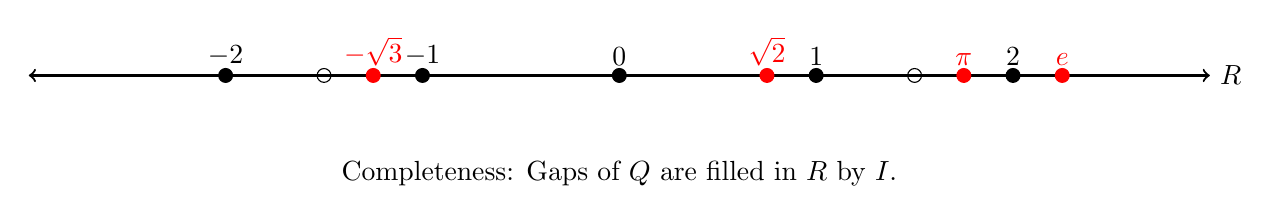
\begin{tikzpicture}[scale=1.25]
        % Draw the real number line with arrows in both directions
        \draw[thick,<->] (-6,0) -- (6,0) node[right] {$\mathbb{R}$};
        
        % Place some rational numbers (randomly chosen for illustration)
        \foreach \x/\label in {-4/$-2$, -2/$-1$, 0/$0$, 2/$1$, 4/$2$} {
            \filldraw (\x,0) circle (2pt) node[above] {\label};
        }
        
        % Gaps (represented as empty circles)
        \foreach \x in {-3, 3} {
            \draw (\x,0) circle (2pt);
        }
        
        % Pointing out some irrational and transcendental numbers
        \filldraw[red] (-2.5,0) circle (2pt) node[above] {$-\sqrt{3}$};
        \filldraw[red] (1.5,0) circle (2pt) node[above] {$\sqrt{2}$};
        \filldraw[red] (3.5,0) circle (2pt) node[above] {$\pi$};
        \filldraw[red] (4.5,0) circle (2pt) node[above] {$e$};
        
        % Label for completeness
        \node at (0,-1) {Completeness: Gaps of $\mathbb{Q}$ are filled in $\mathbb{R}$ by $\mathbb{I}$.};
    \end{tikzpicture}
\end{center}
\noindent This visualization is intuitive, but we still need a rigorous proof of the existence of gaps in the rational number line.
\begin{Example}\label{gaps_in_rationals}
    Gaps Exist in the Rational Numbers.
\end{Example}
\noindent\begin{proof}
    Let us define the following two sets:
$$A=\{m\in\mathbb{Q}:m^2<2\},\ B=\{p\in\mathbb{Q}:p^2>2\}$$
If we can always find a rational number, $n$, that has the properties $n^2<2$ and $n>m$ (i.e. $\sqrt{2}>n>m$) for any choice of $m\in A$, then it proves the existence of gaps in the rational numbers.\\
Now, any choice of $m$ adheres by $m^2<2\implies2-m^2>0$. However, we need to show that $n$ is larger than $m$. So, we need $n=m+f(2-m^2)$ where $f(2-m^2)>0$.\footnotemark\\
\footnotetext{The reason for writing $f(2-m^2)$ instead of $f(m)$ is just my own choice; the readers can denote the function as the function of $2-m^2$ or $m$ as they please.}
\noindent Again,
\begin{align}
    & 2>n^2>m^2\nonumber\\
    \implies& 2-m^2>n^2-m^2>0\nonumber\\
    \implies& 2-m^2>(n+m)(n-m)>0\nonumber\\
    \implies& 2-m^2>\{2m+f(2-m^2)\}f(2-m^2)>0\nonumber\\
    \implies& \frac{2-m^2}{f(2-m^2)}>2m+f(2-m^2)>0\nonumber\\
    \implies& \frac{2-m^2}{f(2-m^2)}>2m+f(2-m^2)>2m>0\nonumber\\
    \implies& \boxed{\frac{2-m^2}{2m}>f(2-m^2)>0}\nonumber
\end{align}
Another piece of information we have is that,
\begin{equation*}
    2>\sqrt{2}>m\implies 2>m\implies m+2>2m\implies \frac{1}{2m}>\frac{1}{m+2}\implies \boxed{\frac{2-m^2}{2m}>\frac{2-m^2}{m+2}}
\end{equation*}
So, combining both boxed equations, we can define\footnotemark\footnotetext{The symbol $:=$ is used when defining something in mathematics.} $$\boxed{f(2-m^2):=\frac{2-m^2}{m+2};\ n=m+\frac{2-m^2}{m+2}}$$

Now we will verify the properties we are seeking.
$$n=m+f(2-m^2)\implies n-m=f(2-m^2)=\frac{2-m^2}{m+2}>0\implies n>m$$
\begin{align*}
    2-n^2&=(\sqrt{2})^2-n^2=(\sqrt{2}+n)(\sqrt{2}-n)=\big(\sqrt{2}+m+\frac{2-m^2}{m+2}\big)\big(\sqrt{2}-m-\frac{2-m^2}{m+2}\big)\\
    &=\big(\sqrt{2}+\frac{2(m+1)}{m+2}\big)\big(\sqrt{2}-\frac{2(m+1)}{m+2}\big)=2-\frac{4(m+1)^2}{(m+2)^2}=\frac{2}{(m+2)^2}\big((m+2)^2-2(m+1)^2\big)\\
    &=\frac{2}{(m+2)^2}(2-m^2)>0\\
    \implies2-n^2 &>0
\end{align*}
As we can always construct $n$ from any arbitrary choice of $m$ (It is the arbitrary choice that gives generality to the statement we are trying to prove), there will always exist a rational number $\sqrt{2}>n>m$ and $n\in A$. This proves the existence of gaps in the rational numbers utilizing the set $A$. What can be done for the set $B$?
\end{proof}
\exercise
\begin{enumerate}
    \item \textbf{Prove that $\pmb{\sqrt{3}}$ is an Irrational Number.}
    \item \textbf{Prove that $\pmb{\sqrt{6}}$ is an Irrational Number.}
    \item \textbf{If $\pmb{a^2}$ is an odd number, then prove that $\pmb{a}$ is also an odd number. Prove it using the method used in the \pmb{\cref{fnt1}} and then prove it again by using the method of contradiction.}
    \item \textbf{What happens if one tries proving $\pmb{\sqrt{4}}$ as an irrational number in the same way as $\pmb{\sqrt{2}}$? Explain what goes wrong, if there is any!} 
    \item \textbf{Prove the existence of gaps in the rational numbers using set $\pmb{B}$ by constructing a rational number $\pmb{q}$ such that $\pmb{p>q>\sqrt{2}}$ in the same way we have shown for set $\pmb{A}$ in example \pmb{\eqref{gaps_in_rationals}}.}
\end{enumerate}
\section{Completeness}
In this section, we will investigate the completeness property more deeply. For that, we at first have to go back and see what type of set makes completeness apparent, just like example \eqref{gaps_in_rationals}. Now we want to study a broader class of such examples first, so that we can be precise about any assertions regarding completeness.
\subsection{Bounded Sets, Supremum \& Infimum of Sets}
A general prescription of the type of set in example \eqref{gaps_in_rationals} is given below:
\begin{Definition}{Bounded Sets}\label{bounded_sets}
    Let $A$ be a non-empty subset of $\mathbb{R}$, then the set $A$ will be called bounded if there exist two real numbers $a, b\footnotemark$ and $a\leq b$ such that for all $x\in A$, we get $a\leq x\leq b$.\\
    If the set $A$ satisfies the condition $a\leq x$ only, for all $x\in A$, then the set $A$ is called a \textbf{bounded below} set and the number $a$ is called a \textbf{lower bound}.\\
    If the set $A$ satisfies the condition $x\leq b$ only, for all $x\in A$, then the set $A$ is called a \textbf{bounded above} set and the number $b$ is called an \textbf{upper bound}.
\end{Definition}
\footnotetext{Very importantly, notice that the numbers $a, b$ do not necessarily have to be members of the reference set $A$. Also, note that we have not yet introduced the concept of infinity.}
\noindent Now, we want to find the absolute number (or point in the real line) from where the upper bounds and lower bounds start to emerge. A simple solution is to take that upper bound below which no numbers are upper bounds, that is, taking the smallest of the upper bounds. This motivates us to define the following -
\begin{Definition}{Supremum of a Set}\label{supremum}
    An upper bound of a set $A\subset\mathbb{R}$ and $A\neq\varnothing$, denoted by $b$, will be called the supremum of the set $A$ if for all other upper bounds $v$, we get $b\leq v$.\\
    The supremum is denoted by $\sup A=b$ or simply $\sup A$.
\end{Definition}
\noindent Thinking similarly for the lower bounds gives us the infimum.
\begin{Definition}{Infimum of a Set}\label{infimum}
    A lower bound of a set $A\subset\mathbb{R}$ and $A\neq\varnothing$, denoted by $a$, will be called the infimum of the set $A$ if for all other lower bounds $u$, we get $u\leq a$.\\
    The infimum is denoted by $\inf A=a$ or simply $\inf A$.
\end{Definition}
\noindent One can remember the definitions more easily by the following lines:
\begin{enumerate}
    \item A supremum is the smallest of the upper bounds.
    \item An infimum is the largest of the lower bounds.
\end{enumerate}
Another important thing to consider in the definitions is that the bounds, supremum, and infimum do not have to be members of the set itself.\\
\textbf{Although the concepts of upper and lower bounds are introduced here in the context of a totally ordered set, they can be defined exactly the same in the context of a preordered set.}
\subsubsection{Properties of the Supremum}
Before we investigate the properties of the supremum, let us establish some notations.
\begin{align*}
    & A=\{a:a\in A, A\subset\mathbb{R}\},\ cA=\{x:x=ca,\text{ for all }x\in A\text{ and }c\in\mathbb{R} \}\\
    & B=\{b:b\in B, B\subset\mathbb{R}\},\ A+B=\{p:p=a+b,\text{ where }a\in A,b\in B\}\\
    & A\cdot B=\{q:q=a\cdot b,\text{ where }a\in A,b\in B\}\\
    & A\leq B\implies a\leq b,\text{ for all }a\in A, b\in B
\end{align*}
\begin{Theorem}{Uniqueness of Supremum}\label{uniqueness_supremum}
    The supremum of a set, if it exists, is unique.
\end{Theorem}
\begin{proof}
    Let $s_1, s_2$ be two suprema of a non-empty subset of real numbers, $A$. Then, both $s_1, s_2$ are upper bounds of the set $A$.\\ 
    Now, $s_1$ by definition of supremum, $\boxed{s_1\leq s_2}$.\\
    Similarly, $s_2$ by definition of supremum, $\boxed{s_2\leq s_1}$. \\
    Combining both boxed equations, we get $s_1=s_2$. So, the supremum of the set $A$ is unique. As $A$ was an arbitrary set, we can say, the supremum is unique.
\end{proof}
\begin{Theorem}{Necessary and Sufficient Conditions of Supremum}\label{iff_supremum}
    Let $A\subset\mathbb{R}$ and $A\neq\varnothing$, then following are the necessary and sufficient conditions for $\sup A=s$:
    \begin{enumerate}
        \item For all $x\in A$, $x\leq s$.
        \item For any $\epsilon>0, \epsilon\in\mathbb{R}$, there exists at least one $x\in A$ such that $s-\epsilon<x$.\footnotemark
    \end{enumerate}
    [Check \pmb{\cref{iff_statement}} for the meaning of necessary and sufficient conditions.]
\end{Theorem}
\footnotetext{Congratulations! This is your first exposure to the famous epsilon ($\epsilon$) in analysis. Remember this number very vividly, because we will have numerous encounters with this throughout our analysis journey.}
\begin{proof}
    For the forward direction $(\implies)$, we have to start by assuming that $\sup A = s$ and then prove the two conditions. \\
    The supremum is an upper bound by definition, and therefore, for all $x\in A, x\leq s$ is true by the definition of an upper bound. \\
    Now, for the second condition, for the sake of contradiction, let us assume there exists no such $x\in A$ for which $s-\epsilon<x$.  That is, we consider for any $\epsilon>0$ such that $x\leq s-\epsilon$ for all $x \in A$. So, $s-\epsilon$ is an upper bound. As $s$ is the supremum, then 
    \begin{align*}
        & s\leq s-\epsilon\\
        \implies & 0\leq -\epsilon\\
        \implies & \epsilon \leq 0
    \end{align*}
    This is clearly not true, and so we must have at least one $x\in A$ such that $s-\epsilon<x$. This proves the second condition. So, we have proved the forward direction $(\implies)$. \\
    As for the backward direction $(\impliedby)$, we have to start by assuming the two conditions to be true and then prove that $\sup A = s$. \\
    By the first condition, we know that $s$ is an upper bound by definition.\\
    As for the second condition, for the sake of contradiction, let us assume that $s$ is not the supremum, and then, there exists another upper bound $s'<s$. Then, $s-s'>0$, and let us set $\epsilon=s-s'$. Then, by the second condition, $s-\epsilon=s-s+s'<x\implies s'<x$. This means that $s'$ is not an upper bound. So, no such $s'<s$ exists, that means all upper bounds follow $s\leq s'$. Thus, the second condition along with the first condition proves that $\sup A = s$.\\ This completes the backwards $(\impliedby)$ proof.
\end{proof}
\begin{Theorem}{Positive Scalar Product of Supremum\footnotemark}\label{positive_scalar_product_supremum}
    Let $A$ be a non-empty proper subset of $\mathbb{R}$, with supremum $\sup A=s$, then for $c>0,\ c\in\mathbb{R}$, $$\sup (cA)=c\sup A=cs$$
\end{Theorem}
\footnotetext{In mathematics, product by a constant number is called \textit{scalar product}.}
\begin{proof}
    By definition of the supremum, for all $a\in A$,
    \begin{align*}
        & a\leq \sup A \\
        \implies & ca\leq c\sup A
    \end{align*}
    So, $c\sup A$ is an upper bound for the set $cA$.\\
    Again, by definition of the upper bound, for all upper bounds $M$ of the set $cA$, for all $a\in A$,
    \begin{align*}
        & ca\leq M\\
        \implies& a\leq\frac{M}{c}
    \end{align*}
    As $\sup A$ is the least upper bound, by definition we get,
    \begin{align*}
        &\sup A\leq\frac{M}{c}\\
        \implies& c\sup A\leq M
    \end{align*}
    By definition of the supremum, we get $\sup(cA)=c\sup A$.
\end{proof}
\begin{Theorem}{Addition of Supremum}\label{addition_supremum}
    Let $A, B$ be non-empty proper subsets of $\mathbb{R}$, with their supremum $\sup A= s,\sup B=t$. Then, $$\sup (A+B)=\sup A+\sup B=s+t$$
\end{Theorem}
\begin{proof}
    By definition of the supremum,
    \begin{align*}
        & a\leq\sup A,\text{ for all }a\in A\ \&\ b\leq\sup B,\text{ for all }b\in B\\
        \implies &a+b\leq\sup A+\sup B,\text{ for all }a\in A, b\in B
    \end{align*}
    So, $\sup A+\sup B$ is an upper bound of the set $(A+B)$.\\
    Let $M$ be an arbitrary upper bound of $(A+B)$. Then,
    \begin{align*}
        &a+b\leq M,\text{ for all }a\in A,b\in B\\
        \implies&b\leq M-a,\text{ for all }a\in A,b\in B
    \end{align*}
    So, $M-a$ is an upper bound of the set $B$, then by definition of the supremum,
    \begin{align*}
        &\sup B\leq M-a,\text{ for all }a\in A\\
        \implies&a\leq M-\sup B,\text{ for all }a\in A
    \end{align*}
    Again, $M-\sup B$ is an upper bound of the set $A$, then by definition of the supremum,
    \begin{align*}
        &\sup A\leq M-\sup B\\
        \implies&\sup A+\sup B\leq M
    \end{align*}
    As $M$ was an arbitrary upper bound of $(A+B)$, by definition of the supremum, we can say that, $$\sup(A+B)=\sup A+\sup B$$ This concludes the proof.
\end{proof}
\begin{Theorem}{Product of Supremum}\label{product_supremum}
    Let $A, B$ be non-empty proper subsets of $\mathbb{R}$, with their supremum $\sup A = s,\sup B=t$. Then, $$\sup (A\cdot B)=\sup A\cdot\sup B=s\cdot t$$
\end{Theorem}
\begin{proof}
    By definition of the supremum,
    \begin{align*}
        & a\leq\sup A,\text{ for all }a\in A\ \&\ b\leq\sup B,\text{ for all }b\in B\\
        \implies &a\cdot b\leq\sup A\cdot\sup B,\text{ for all }a\in A, b\in B
    \end{align*}
    So, $\sup A\cdot\sup B$ is an upper bound of the set $(A\cdot B)$.\\
    Let $M$ be an arbitrary upper bound of $(A\cdot B)$. Then,
    \begin{align*}
        &a\cdot b\leq M,\text{ for all }a\in A,b\in B\\
        \implies&b\leq \frac{M}{a},\text{ for all }a\neq 0,a\in A,b\in B
    \end{align*}
    So, $\frac{M}{a}$ is an upper bound of the set $B$, then by definition of the supremum,
    \begin{align*}
        &\sup B\leq \frac{M}{a},\text{ for all }a\neq0,a\in A\\
        \implies&a\leq \frac{M}{\sup B},\text{ for all }a\in A,\sup B\neq 0
    \end{align*}
    Again, $\frac{M}{\sup B}$ is an upper bound of the set $A$, then by definition of the supremum,
    \begin{align*}
        &\sup A\leq \frac{M}{\sup B}\\
        \implies&\sup A\cdot\sup B\leq M
    \end{align*}
    As $M$ was an arbitrary upper bound of $(A\cdot B)$, by definition of the supremum, we can say that, $$\sup(A\cdot B)=\sup A\cdot \sup B$$ This concludes the proof.
\end{proof}
\begin{Theorem}{Supremum and Order}\label{supremum_order}
    Let $A, B$ be non-empty proper subsets of $\mathbb{R}$, with their supremum $\sup A = s,\sup B=t$. Then, $$A\leq B\implies\sup A\leq\sup B\implies s\leq t$$
\end{Theorem}
\begin{proof}
    By definition of the supremum, we have,
    $$a\leq\sup A,\text{ for all }a\in A,\ b\leq\sup B,\text{ for all }b\in B$$
    Now, as $a\leq b,\text{ for all }a\in A, b\in B$, we have $a\leq b\leq\sup B\implies a\leq\sup B$ for all $a\in A$. So, $\sup B$ is an upper bound of $A$.\\
    By definition of the supremum, $\sup A\leq M$, where $M$ is any upper bound of $A$. Setting $M=\sup B$, we get $\sup A\leq\sup B$.\\
    This concludes the proof.
\end{proof}
\subsubsection{Properties of the Infimum}
\begin{Theorem}{Uniqueness of Infimum}\label{uniqueness_infimum}
    The infimum of a set, if it exists, is unique.
\end{Theorem}
\begin{proof}
    Let $i_1, i_2$ be two infima of a non-empty subset of real numbers, $A$. Then, both $i_1, i_2$ are lower bounds of the set $A$.\\ 
    Now, $i_1$ by definition of infimum, $\boxed{i_1 \geq i_2}$.\\
    Similarly, $i_2$ by definition of infimum, $\boxed{i_2 \geq i_1}$. \\
    Combining both boxed equations, we get $i_1 = i_2$. So, the infimum of the set $A$ is unique. As $A$ was an arbitrary set, we can say, the infimum is unique.
\end{proof}

\begin{Theorem}{Necessary and Sufficient Conditions of Infimum}\label{iff_infimum}
    Let $A\subset\mathbb{R}$ and $A\neq\varnothing$, then following are the necessary and sufficient conditions for $\inf A = i$:
    \begin{enumerate}
        \item For all $x\in A$, $x \geq i$.
        \item For any $\epsilon > 0, \epsilon\in\mathbb{R}$, there exists at least one $x\in A$ such that $x < i + \epsilon$.
    \end{enumerate}
\end{Theorem}
\begin{proof}
    For the forward direction $(\implies)$, assume $\inf A = i$. \\
    The infimum is a lower bound by definition, so for all $x\in A$, $x \geq i$ holds. \\
    For the second condition, suppose for contradiction that there exists $\epsilon > 0$ such that $x \geq i + \epsilon$ for all $x \in A$. Then $i + \epsilon$ is a lower bound. Since $i$ is the infimum:
    \begin{align*}
        & i \geq i + \epsilon \\
        \implies & 0 \geq \epsilon
    \end{align*}
    This is clearly not true, and so we must have at least one $x\in A$ such that $x < i + \epsilon$. This proves the second condition. \\
    For the backward direction $(\impliedby)$, assume the two conditions hold. By (1), $i$ is a lower bound. Suppose there exists another lower bound $i' > i$. Let $\epsilon = i' - i > 0$. By (2), there exists $x \in A$ with $x < i + \epsilon = i'$, contradicting that $i'$ is a lower bound. Thus $i$ is the greatest lower bound.
\end{proof}

\begin{Theorem}{Positive Scalar Product of Infimum}\label{positive_scalar_product_infimum}
    Let $A$ be a non-empty proper subset of $\mathbb{R}$, with infimum $\inf A = i$, then for $c > 0,\ c\in\mathbb{R}$, $$\inf (cA) = c\inf A = ci$$
\end{Theorem}
\begin{proof}
    By definition of the infimum, for all $a\in A$,
    \begin{align*}
        & a \geq \inf A \\
        \implies & ca \geq c\inf A
    \end{align*}
    So, $c\inf A$ is a lower bound for the set $cA$.\\
    For any lower bound $m$ of $cA$, for all $a\in A$,
    \begin{align*}
        & ca \geq m\\
        \implies & a \geq \frac{m}{c}
    \end{align*}
    As $\inf A$ is the greatest lower bound, by definition we get,
    \begin{align*}
        &\inf A \geq \frac{m}{c}\\
        \implies & c\inf A \geq m
    \end{align*}
    By definition of the infimum, we get $\inf(cA) = c\inf A$.
\end{proof}

\begin{Theorem}{Addition of Infimum}\label{addition_infimum}
    Let $A, B$ be non-empty proper subsets of $\mathbb{R}$, with their infimum $\inf A= i,\inf B=j$. Then, $$\inf (A+B)=\inf A+\inf B=i+j$$
\end{Theorem}
\begin{proof}
    By definition of the infimum,
    \begin{align*}
        & a\geq\inf A,\text{ for all }a\in A\ \&\ b\geq\inf B,\text{ for all }b\in B\\
        \implies &a+b\geq\inf A+\inf B,\text{ for all }a\in A, b\in B
    \end{align*}
    So, $\inf A+\inf B$ is a lower bound of the set $(A+B)$.\\
    Let $m$ be an arbitrary lower bound of $(A+B)$. Then,
    \begin{align*}
        &a+b\geq m,\text{ for all }a\in A,b\in B\\
        \implies&b\geq m-a,\text{ for all }a\in A,b\in B
    \end{align*}
    So, $m-a$ is a lower bound of the set $B$, then by definition of the infimum,
    \begin{align*}
        &\inf B\geq m-a,\text{ for all }a\in A\\
        \implies&a\geq m-\inf B,\text{ for all }a\in A
    \end{align*}
    Again, $m-\inf B$ is a lower bound of the set $A$, then by definition of the infimum,
    \begin{align*}
        &\inf A\geq m-\inf B\\
        \implies&\inf A+\inf B\geq m
    \end{align*}
    As $m$ was an arbitrary lower bound of $(A+B)$, by definition of the infimum, we can say that, $$\inf(A+B)=\inf A+\inf B$$ This concludes the proof.
\end{proof}

\begin{Theorem}{Product of Infimum}\label{product_infimum}
    Let $A, B$ be non-empty proper subsets of $\mathbb{R}$, with their infimum $\inf A = i,\inf B=j$. Then, $$\inf (A\cdot B)=\inf A\cdot\inf B=i\cdot j$$
\end{Theorem}
\begin{proof}
    By definition of the infimum,
    \begin{align*}
        & a\geq\inf A,\text{ for all }a\in A\ \&\ b\geq\inf B,\text{ for all }b\in B\\
        \implies &a\cdot b\geq\inf A\cdot\inf B,\text{ for all }a\in A, b\in B
    \end{align*}
    So, $\inf A\cdot\inf B$ is a lower bound of the set $(A\cdot B)$.\\
    Let $m$ be an arbitrary lower bound of $(A\cdot B)$. Then,
    \begin{align*}
        &a\cdot b\geq m,\text{ for all }a\in A,b\in B\\
        \implies&b\geq \frac{m}{a},\text{ for all }a\neq 0,a\in A,b\in B
    \end{align*}
    So, $\frac{m}{a}$ is a lower bound of the set $B$, then by definition of the infimum,
    \begin{align*}
        &\inf B\geq \frac{m}{a},\text{ for all }a\neq0,a\in A\\
        \implies&a\geq \frac{m}{\inf B},\text{ for all }a\in A,\inf B\neq 0
    \end{align*}
    Again, $\frac{m}{\inf B}$ is a lower bound of the set $A$, then by definition of the infimum,
    \begin{align*}
        &\inf A\geq \frac{m}{\inf B}\\
        \implies&\inf A\cdot\inf B\geq m
    \end{align*}
    As $m$ was an arbitrary lower bound of $(A\cdot B)$, by definition of the infimum, we can say that, $$\inf(A\cdot B)=\inf A\cdot \inf B$$ This concludes the proof.
\end{proof}

\begin{Theorem}{Infimum and Order}\label{infimum_order}
    Let $A, B$ be non-empty proper subsets of $\mathbb{R}$, with their infimum $\inf A = i,\inf B=j$. Then, $$A\leq B\implies\inf A\leq\inf B\implies i\leq j$$
\end{Theorem}
\begin{proof}
    By definition of the infimum, we have,
    $$a\geq\inf A,\text{ for all }a\in A,\ b\geq\inf B,\text{ for all }b\in B$$
    Now, as $a\leq b$ for all $a\in A, b\in B$, we have $\inf A\leq a\leq b\implies \inf A\leq b$ for all $b\in B$. So, $\inf A$ is a lower bound of $B$.\\
    By definition of the infimum, $m\leq\inf B$, where $m$ is any lower bound of $B$. Setting $m=\inf A$, we get $\inf A\leq \inf B$.\\
    This concludes the proof.
\end{proof}
\subsubsection{Connection between Supremum and Infimum}
\begin{Theorem}{Supremum and Infimum Inequality}\label{sup_inf_inequality}
    Let $A\subseteq\mathbb{R}$ and $A\neq\varnothing$. Then, $\inf A\leq\sup A$.
\end{Theorem}
\begin{proof}
    By definition of the supremum and infimum,
    \begin{align*}
        & \inf A\leq a\ \&\ a\leq \sup A\text{ for all }a\in A\\
        \implies& \inf A\leq \sup A
    \end{align*}
    This concludes the proof.
\end{proof}
\begin{Theorem}{Infimum in terms of Supremum}\label{infimum_in_terms_of_supremum}
    Let $A\subseteq\mathbb{R}$ and $A\neq\varnothing$. Then, $\inf A=-\sup(-A)$.
\end{Theorem}
\begin{proof}
    Let $\sup(-A)=s\implies-a\leq s\text{ for all }a\in A\implies-s\leq a\text{ for all }a\in A$.\\
    So, $-\sup(-A)=-s$ is a lower bound of $A$.\\
    Again, as $\sup(-A)=s$ implies that for any $\epsilon>0$, there exists at least one $a\in A$ such that $s-\epsilon< -a\implies a<-s+\epsilon$.\\
    Now, by theorem \eqref{iff_infimum}, we see that $-\sup(-A)=-s$ satisfies the necessary and sufficient condition for the infimum of the set $A$.\\
    Therefore, $\inf A=-\sup(-A)$.
\end{proof}
\begin{Theorem}{Negative Scalar Product of the Supremum and Infimum}\label{negative_scalar_product_supremum_infimum}
    Let $A$ be a non-empty proper subset of $\mathbb{R}$, with supremum $\sup A=s$, then for $c<0,\ c\in\mathbb{R}$, $$\sup(cA)=c\inf(A)$$ $$\inf(cA)=c\sup(A)$$
\end{Theorem}
\begin{proof}
    As $c<0$, we can write $c$ as $c=-p$ where $p>0$. Then, we need to prove $\sup(-pA)=-p\inf(A)$ and $\inf(-pA)=-p\sup(A)$.\\
    Now, by theorem \eqref{infimum_in_terms_of_supremum}, we know that $\inf A=-\sup(-A)$. From the positive scalar product of both supremum and infimum, we know that $\sup(pA)=p\sup A$ and $\inf(pA)=p\inf A$. Now,
    \begin{align*}
        & \inf A=-\sup(-A)\\
        \implies& -\inf A=\sup(-A)\\
        \implies& -p\inf(A)=p\sup(-A)\\
        \implies&\sup(-pA)=-p\inf(A)\\
        \implies&\boxed{\sup(cA)=c\inf(A)}
    \end{align*}
    Again, $-(-A)=A$, so setting $A=-A$ (This is just a substitution, not an equation!) gives $\inf(-A)=-\sup(A)$.
    Like before,
    \begin{align*}
        &\inf(-A)=-\sup\big(-(-A)\big)\\
        \implies&\inf(-A)=-\sup(A)\\
        \implies&p\inf(-A)=-p\sup(A)\\
        \implies&\inf(-pA)=-p\sup(A)\\
        \implies&\boxed{\inf(cA)=c\sup(A)}
    \end{align*}
    This concludes the proof.
\end{proof}
\exercise
\begin{enumerate}[label=\textbf{\arabic*.}]
    \item \textbf{Supremum, Infimum and Preordering:} Let $(K,\lesssim)$ be a preordered set. Then define the following in the context of $(K,\lesssim)$:
    \begin{enumerate}
        \item Bounded set, upper bound and lower bound.
        \item Supremum and infimum of the set.
    \end{enumerate}
    [Hint: Read the last line of the part discussing supremum and infimum.]
    \item \textbf{Supremum, Infimum and Subsets:} Let $A,B$ be non-empty bounded subsets of $\mathbb{R}$ and $B\subseteq A$. Then prove the following:
    \begin{enumerate}
        \item $\sup(B)\leq\sup(A)$.
        \item $\inf(A)\leq\inf(B)$.
        \item $\inf(A)\leq\inf(B)\leq\sup(B)\leq\sup(A)$.
    \end{enumerate}
    \item \textbf{Supremum, Infimum, Unions and Intersections:} Let $A,B$ be non-empty bounded subsets of $\mathbb{R}$. Then prove the following:
    \begin{enumerate}
        \item $\inf(A\cup B)\leq\inf(A)$ and $\inf(A\cup B)\leq\inf(B)$.
        \item $\sup(A\cup B)\geq\sup(A)$ and $\sup(A\cup B)\geq\sup(B)$.
        \item $\inf(A\cap B)\geq\inf(A)$ and $\inf(A\cap B)\geq\inf(B)$.
        \item $\sup(A\cap B)\leq\sup(A)$ and $\sup(A\cap B)\leq\sup(B)$.
    \end{enumerate}
    \item \textbf{Simple Computation:} Compute the supremum and infimum (if they exist) of the following sets:
    \begin{enumerate}
        \item $\frac{1}{n}$ where $n\in\mathbb{N}$.
        \item $\frac{n}{m+n}$ where $n,m\in\mathbb{N}$.
        \item $\frac{an}{bn+c}$ where $a,b,c\in\mathbb{R}$, $a, b, c>0$, and $n\in\mathbb{N}$.
        \item $(-1)^n\frac{an}{bn+c}$ where $a,b,c\in\mathbb{R}$, $a, b, c>0$, and $n\in\mathbb{N}$.
    \end{enumerate}
    \item \textbf{Supremum and Infimum of the Empty Set:} In our discussion of the supremum and infimum, we have always assumed our reference set $A\neq\varnothing$, but what will be the case when $A=\varnothing$? In this exercise, we will work through to find the solution step by step.
    \begin{enumerate}
        \item What are the upper bounds and lower bounds of the empty set?\newline
        [Hint: It is time to introduce another trick, vacuous truth, into our analysis repertoire. The trick is given below.]
        \begin{Trick}{Vacuous Truth}\label{vacuous_truth}
            When and where to use this?
            \begin{itemize}
                \item Mainly when proving something for the empty sets, and the property that we wish to prove makes no sense for empty sets.
                \item Most of the time, when a statement for no member or every member of the set cannot be verified exactly.
            \end{itemize}
            \smallskip
            Structure of this proof:\\
            A statement of the form:  for all \(x\in S\) such that \(P(x)\implies Q(x)\), is said to be vacuously true if there are \underline{no elements in \(S\) for which \(P(x)\) is true}. That is, for all $x\in S, \neg P(x)$ is true, and this implies that $P(x)$ is never true. Then, we cannot say anything about $Q(x)$ because, as $P(x)$ is always false, $Q(x)$ can be either true or false. Thus, the statement $P(x)\implies Q(x)$ is taken to be true.\\
            This is the mathematician's way of taking things as granted. Who said mathematicians are skeptical and snobby?\\
            \newline
            A simple example:\\
            There are no students in the classroom. So, let us take a look at the following statements -
            \begin{enumerate}
                \item All students were present.
                \item No student was present.
            \end{enumerate}
            Both of them make no sense as there are no students to begin with, and neither statement can be proved nor disproved. Here, $x$ denotes the students, $P(x)$ denotes the number of students, and $Q(x)$ denotes the presence of the students. So, vacuously, $P(x)\implies Q(x)$ is true for all $x\in S$, meaning that a class having $0$ students implies that all students were present is a vacuously true statement.
        \end{Trick}
        \item Now, if you have managed to solve the first step, then we need to find such numbers that are less than the upper bounds and greater than the lower bounds for determining the supremum and infimum, respectively. Do such numbers exist?
        \item If such numbers do exist, then our work is done, but if they do not exist, then what concept do we need to introduce? After introducing that concept, can it be regarded as a member of the field of real numbers?
    \end{enumerate}
    This whole exercise is a foreshadowing of a very important concept that we will see in this chapter.
    \item \textbf{An off-beat way of identifying the empty set:} Let $A\subset\mathbb{R}$ be a bounded set. Then $\inf(A)\leq\sup(A)$ will be true if and only if $A\neq\varnothing$. 
\end{enumerate}
\subsection{The Maximum and Minimum of Sets}
\subsection{The Axiom of Completeness and its Consequences}
\section{Real Numbers and the Extended Real Numbers}
\subsection{Real Numbers}
\begin{Trick}{Contrapositive Statements}\label{contrapositive_proof}
    When and where to use this?\\
    Mainly when the opposite direction of a proof is significantly easier than the original direction. In other terms, if we wish to prove $P\implies Q$, but we know very little or can infer little from $P$, but we know a lot of things about $Q$, then the contrapositive is the way to go.\\
    Structure of this proof:\\
    If we have a statement $P\implies Q$, then its contrapositive statement is $\boxed{\neg Q\implies\neg P}$, where $\neg$ means not or negation. The contrapositive statement is equivalent to the original statement. This is proved via the truth table below.
\end{Trick}
\begin{Lemma}{Original Statement and Contrapositive Statement}\label{original_and_contrapositive_statement}
        The original statement and the contrapositive statement are the same in logic.
\end{Lemma}
\begin{lemma_proof}
    Some things to learn at first:
    \begin{enumerate}
        \item In $P\implies Q$, when $P$ is false, regardless of the value of $Q$, we have $P\implies Q$ being true. This is because $P$ is the precedent, and if the precedent is not valid (that is, false), then $Q$ is true vacuously. See trick \eqref{vacuous_truth} for a refresher. The same applies to the rest of the statements in this proof.
        \item As both $A\implies B$ and $B\implies A$ are true regardless of the value of the inputs, we can conclude that $A\iff B$.
    \end{enumerate}
    The truth table is as follows:
    \begin{table}[h!]
        \centering
        \scalebox{0.675}{\begin{tabular}{|c|c|c|c|c|c|c|c|}
            \hline
            $P$ & $Q$ & $\neg P$ & $\neg Q$ & $A:=(P\implies Q)$ & $B:=(\neg Q\implies\neg P)$ & $A\implies B$ & $B\implies A$\\\hline
            $T$ & $T$ & $F$ & $F$ & $T$ & $T$ & $T$ & $T$\\\hline
            $T$ & $F$ & $F$ & $T$ & $F$ & $F$ & $T$ & $T$\\\hline
            $F$ & $T$ & $T$ & $F$ & $T$ & $T$ & $T$ & $T$\\\hline
            $F$ & $F$ & $T$ & $T$ & $T$ & $T$ & $T$ & $T$\\\hline
        \end{tabular}}
    \end{table}
    \newline This concludes the proof of the original statement, and the contrapositive statement is logically equivalent.
\end{lemma_proof}
\subsection{Extended Real Numbers}
\section{Complex Numbers and the Extended Complex Numbers}
\subsection{Complex Numbers}
\subsection{Extended Complex Numbers}
\section{Metric Spaces}
\subsection{Definition and Examples of Metric Spaces}
\subsection{Properties of Metric Spaces}
\section{Cardinality of Sets}
In our mathematics journey, we use sets quite extensively, we work with sets of different sizes, some sets have no members like the empty set, some have 3 members like $\{1,2,3\}$, some have infinite members like $\mathbb{N}=\{1,2,3,\dots\}$. This notion of the number of members of the set is called the cardinality of the set.
\subsection{The Basics}
\begin{Definition}{Cardinality of a Set}\label{cardinality}
    The number of elements of a set is defined as the cardinality of that set. For a reference set $A$, the cardinality of the set $A$ is denoted by $|A|$.
\end{Definition}
\noindent Now, based on counting the number of elements of a set, sets are classified into two types:
\begin{enumerate}
    \item Finite Set.
    \item Infinite Set.
\end{enumerate}
\begin{Definition}{Finite Set}\label{finite_set}
    A set is called finite if there is a finite number of elements, that is, the counting of the number of elements of the set stops after a certain time. The cardinality of the finite set can be expressed as a natural number. That is if $A$ is finite, then $|A|=n$ where $n\in\mathbb{N}$.\\ Some classic examples of finite sets are sets like $\{1,2\},\ \{1,2,3,\dots,420\},\ \{x,y,z,p,q,r,s,t\}$ which have cardinality 2, 420, and 8, respectively.
\end{Definition}
\begin{Definition}{Infinite Set}\label{infinite_set}
    A set is called infinite if there are an infinite number of elements, that is, the counting of the number of elements of the set never stops. The cardinality of the infinite set cannot be expressed as a natural number. That is if $A$ is infinite, then $|A|\neq n$ where $n\in\mathbb{N}$.\\
    Some classic examples of infinite sets are sets like $\mathbb{N,\ Z,\ Q,\ I,\ R,\ C}$. The cardinality of the naturals has a special symbol denoted by $|\mathbb{N}|=\aleph_0$ (Pronounced as `aleph zero').
\end{Definition}
\subsubsection{Countable Sets: Bigger \& Smaller Infinite Sets?!}
Mathematicians are a funny group of people; they always try to find new methods to extend the domain of certain ideas. By directly counting the number of elements, one can easily differentiate between the finite and infinite sets. However, what happens if we try to count the sizes of two infinite sets? It seems that our method of direct counting will fail, as for both infinite sets, the counting will never stop. So, we need a new (and indirect!) method of counting. One of the most common method of indirect test we see in our daily lives is the test by comparison. But this test, by comparison, presents us with two new questions, namely
\begin{enumerate}
    \item What will be the standard for comparison?
    \item What will be the process of comparison?
\end{enumerate}
Let us try to answer the second question first! As we are working in the confines of set theory, it is no surprise that our method of comparison will involve a function, but what type of function is the million-dollar question! When we try to compare two infinite sets, say $A$ and $B$, using a function $f$, to ensure that they are of the same size (the comparison will hold when they are of same size, if they are not of the same size the comparison will not hold and so we cannot infer any new information from that case), we must check two things first:
\begin{enumerate}
    \item Both $A, B$ are of the same size, so if we remove one member of the set $A$ as the input of the function, then it should also mean that we will be able to remove the corresponding member of the set $B$. This means that the function must be one-one or injective.
    \item $f(A)=B$, the function must be onto or surjective because, as they are of the same size, we cannot have the image of the function include more or less members than the set $B$.
\end{enumerate}
This means that \textbf{our function for size comparison has to be bijective or one-to-one correspondence}. A wonderful detail about bijective functions is stated without proof (the readers are implored to work it out by themselves) as follows -
\begin{Theorem}{Bijective Functions and Inverse Functions}\label{bijective_and_inverse}
    The inverse of a function exists, if and only if the function is bijective.
\end{Theorem}
\noindent So, when comparing the sizes of two sets $A, B$, if we can find a one-to-one correspondence or a bijective function $f: A \to B$, then we can say that the sets have the same cardinality. Now that we have managed to find the process of comparison for infinite sets, we must also check if it holds for finite sets. If it does not, then all our work attempting to generalize the counting process will fail. But fortunately, the readers can verify (quite easily too, but it is still kept as one of the exercises) that this comparison holds true for finite sets too!\\
Now we try to set the standard of comparison for infinite sets. In our journey, we have encountered some seriously important numbers such as $\mathbb{N,\ Z,\ Q,\ R, C}$. But infinities are not fun to work with, as you have seen before in the consequences of the axiom of completeness section. This gives us the incentive to work with the smallest possible infinite set we can find and by membership alone, we see that $\mathbb{N\subset Z\subset Q\subset R\subset C}$. So, we set our \textbf{standard for infinite sets as the set of natural numbers} $\pmb{\mathbb{N}}$.\\
This wonderful method of generalizing cardinality to infinite sets was put forth by a wonderful Russian-German mathematician named Georg Cantor (1845-1918).
\begin{Definition}{Countably Infinite Set}\label{countably_infinite_set}
    A set $A$ is defined to be countably infinite if its cardinality is exactly equal to the cardinality of the natural numbers, that is, $|A|=|\mathbb{N}|=\aleph_0$.
\end{Definition}
\noindent Now, let us explore some instances to apply our newfound method of counting.
\begin{Example}
    The sets of Even and Odd numbers are countably infinite.
\end{Example}
\begin{proof}
    Let the set of even numbers be denoted by $E=\{2,4,6,8,\dots\}$.\\
    Let the set of odd numbers be denoted by $O=\{1,3,5,7,\dots\}$.\\
    Recall that we have considered $\mathbb{N}=\{1,2,3,\dots\}$.\\
    To prove that the sets $E,\ O$ are countably infinite, we need to show a one-to-one correspondence or bijective function from $\mathbb{N}$ to $E$ and $O$. By theorem \eqref{bijective_and_inverse}, the determination of the inverse alone should suffice!\\
    Now, $E=\{2,4,6,\dots\}$ can be expressed in terms of $\mathbb{N}$ by the function $f_1:\mathbb{N}\to E$ where $$f_1(n)=2n\implies n=\frac{f_1(n)}{2}\implies f^{-1}_1(f_1(n))=\frac{f_1(n)}{2}\implies f^{-1}_1(y)=\frac{y}{2}$$
    Similarly, $O=\{1,3,5,\dots\}$ can be expressed in terms of $\mathbb{N}$ by the function $f_2:\mathbb{N}\to O$ where $$f_2(n)=2n-1\implies n=\frac{f_2(n)+1}{2}\implies f^{-1}_2(f_2(n))=\frac{f_2(n)+1}{2}\implies f^{-1}_2(y)=\frac{y+1}{2}$$
    Therefore, both $E,\ O$ are countably infinite sets.
\end{proof}
\begin{Example}
    The set of Integers is countably infinite.
\end{Example}
\begin{proof}
    Like the previous illustration, we need a bijective function from $\mathbb{N}$ to $\mathbb{Z}$. One way we can accomplish that is to make a function that assigns the even numbers to the positive integers and the odd numbers to the non-positive integers. So, we establish $f : \mathbb{N} \to \mathbb{Z}$ where
    \begin{align*}
        f(n)=\begin{cases}
            \frac{n}{2},\text{ where }n\text{ is even}\\
            -(\frac{n-1}{2}),\text{ where }n\text{ is odd}
        \end{cases}
    \end{align*}
    Just like before, we can construct the inverse function $f^{-1} : \mathbb{Z}\to\mathbb{N}$ where
    \begin{align*}
        f^{-1}(y)=\begin{cases}
            2y,\text{ where }y\text{ is positive integer number}\\
            1-2y,\text{ where }y\text{ is non-positive integer number}
        \end{cases}
    \end{align*}
    This concludes the proof that the set of integers is also countably infinite.
\end{proof}
\noindent \textbf{A very interesting (and bizarre) thing to notice is that} $\pmb{E,O\subset\mathbb{N}\subset\mathbb{Z}}$, \textbf{but} $\pmb{|E|=|O|=|\mathbb{N}|=|\mathbb{Z}|=\aleph_0}$. Upon inspection, one might think that this kind of bizarre characteristic occurs because all involved sets are infinite, and that is actually quite the correct observation. This behavior will motivate us to define an alternate type of finite and infinite sets, which are named after the German mathematician Richard Dedekind (1831-1916).
\begin{Definition}{Dedekind Finite Set}\label{dedekind_finite_set}
    A set is defined as Dedekind finite if the cardinality of the set itself is strictly greater than the cardinality of all of its proper subsets.
\end{Definition}
\noindent Similarly, we define a Dedekind infinite set.
\begin{Definition}{Dedekind Infinite Set}\label{dedekind_infinite_set}
    A set is defined to be Dedekind infinite if the cardinality of the set itself is equal to the cardinality of at least one of its proper subsets.
\end{Definition}
\noindent One might wonder what the relationship is between the two types of finite and infinite sets. Are they equivalent or not? This gives us the next theorem.
\begin{Theorem}{Dedekind Finite Sets \& Finite Sets, Dedekind Infinite Sets \& Infinite Sets}\label{dedekind_finite_sets_and_dedekind_infinite_sets}
    \begin{enumerate}
        \item All finite sets are Dedekind finite sets.
        \item All Dedekind infinite sets are infinite sets.
    \end{enumerate}
\end{Theorem}
\begin{proof}
    (1) By definition of finite set, $|A|=n$ where $n\in\mathbb{N}$. If $B\subset A$ and $A$ is finite, then there exists at least one element $x$ such that $x\in A, x\notin B$. So,
    $B\subseteq A\setminus\{x\}\implies|B|\leq n-1\implies|B|\leq n-1<n=|A|\implies|B|<|A|$. So, we have got for all $B\subset A$, $|B|<|A|$, from $A$ being finite set. So, this concludes the proof that all finite sets are Dedekind finite sets.\\
    (2) This is just the contrapositive statement of (1), and as the original statement \& the contrapositive statement are logically the same, following the proof of (1), (2) is also proved. This concludes the proof of Dedekind infinite sets being infinite sets.
\end{proof}
\noindent \textbf{An interesting thing to note is that it is not as straight forward to prove the opposite direction, that is, proving all Dedekind finite sets are finite sets. This is not as easy as it looks and requires the axiom of choice. As such, it is left for section \eqref{things_involving_the_AoC}.}\\ Now we want to create a new idea of the size of sets that will allow us to combine the usual finite sets with the countably infinite sets. Now, as the cardinality of the naturals is defined as countably infinite, then any other arbitrary set with cardinality less than the naturals should also be countable in some sense, and it also agrees with the finite sets then being countable as well. With that out of the way, we now define a set with a more generalized notion of finiteness.
\begin{Definition}{Countable Sets}\label{countable_sets}
    Let $A$ be an arbitrary set, and it will be defined as countable if the cardinality of $A$ is equal to or less than the cardinality of the naturals. Symbolically, set $A$ is countable if $|A|\leq\aleph_0$.
\end{Definition}
\noindent \underline{\textbf{Some Other Equivalent Definitions of Countable Sets:}} The following are some of the alternate definitions of countable sets..
\begin{Definition}{Alternate Definitions of Countable Sets}\label{alternate_countable_set}
    \begin{enumerate}
        \item An arbitrary set $A$ is countable if there exists a bijective function or map from the set to a subset of the naturals. Symbolically $f:A\xrightarrow{\rm bij}B\subseteq\mathbb{N}$.
        \item An arbitrary set $A$ is countable if there exists an injective function or map from the set to the naturals, i.e., $f:A\xrightarrow{\rm inj}\mathbb{N}$.
        \item An arbitrary set $A$ is countable if there exists a surjective function or map from the naturals to the set, i.e., $f:\mathbb{N}\xrightarrow{\rm sur}A$.
\end{enumerate}
\end{Definition}
\begin{proof}
    Let the original definition be definition 1, with the other alternate definitions being 2, 3, and 4 in the order of their presentation in definition \eqref{alternate_countable_set}.
    \begin{enumerate}
        \item $\pmb{1\iff 3}$\\
        Let us assume the original definition, then for countable sets, $|A|\leq|\mathbb{N}|$. Then by the definition of injective function, there exists an injective function, $f:A\xrightarrow{\rm inj}\mathbb{N}$. So, $1\implies 3$.\\
        Using the same logic in the opposite direction, we can show that $3\implies 1$.
        \item $\pmb{1\iff 2}$\\
        Let us start from the second definition. Then, $B\subseteq\mathbb{N}\implies|B|\leq|\mathbb{N}|=\aleph_0$. By definition $f:A\xrightarrow{\rm bij}B\subseteq\mathbb{N}$ and we know that a bijection preserves the cardinality, i.e., $|A|=|B|$. So, $|B|\leq\aleph_0\implies|A|\leq\aleph_0$. So, $2\implies 1$.\\
        Now let us assume the original definition. As definition $1\iff 3$, by definition 3, we already have an $f:A\xrightarrow{\rm inj}\mathbb{N}$. By definition, $f:A\to f(A)$ is surjective, so let us set $f(A)=B$ and then we get $f:A\xrightarrow{\rm bij}B\subseteq\mathbb{N}$. This proves $1\implies 2$.
        \item $\pmb{1\iff 4}$\\
        \textbf{Left for section \eqref{things_involving_the_AoC} as its proof requires the axiom of choice.}
    \end{enumerate}
    This concludes the proof.
\end{proof}
\begin{Definition}{Uncountable Sets}\label{uncountable_set}
    Let $A$ be an arbitrary set, and it will be defined as uncountable if the cardinality of $A$ is greater than the cardinality of the naturals. Symbolically, set $A$ is uncountable if $|A|>\aleph_0$.\\
    Quite simply, a set that is not countable, is defined as uncountable.
\end{Definition}
\noindent As a small refresher of what we learned in this section, the diagram below is provided:
\begin{center}
    \begin{tikzpicture}[
    node distance=1.5cm and 1cm,
    box/.style={draw, rounded corners, minimum width=2cm, minimum height=0.8cm},
    arrow/.style={-Stealth, semithick}
    ]

        % Level 0: Set Types
        \node[box] (settypes) {Set Types};
    
        % Level 1: Countable and Uncountable
        \node[box, below left=of settypes] (countable) {Countable Sets};
        \node[box, below right=of settypes] (uncountable) {Uncountable Sets};
        
        % Level 2: Under Countable
        \node[box, below left=of countable] (finite) {Finite Sets};
        \node[box, below=of countable] (countinf) {Countably Infinite Sets};
        
        % Level 2: Under Uncountable
        \node[box, below=of uncountable] (uncountinf) {Uncountably Infinite Sets};
        
        % Arrows
        \draw[arrow] (settypes) -- (countable);
        \draw[arrow] (settypes) -- (uncountable);
        \draw[arrow] (countable) -- (finite);
        \draw[arrow] (countable) -- (countinf);
        \draw[arrow] (uncountable) -- (uncountinf);
    \end{tikzpicture}
\end{center}
\subsubsection{Arbitrary Unions, Intersections: A Fun Excursion}
\exercise
\begin{enumerate}[label=\textbf{\arabic*.}]
    \item \textbf{Prove that bijection preserves the cardinality for finite sets.}
    \item \textbf{Prove the following theorem -}
    \begin{Theorem}{Cantor's Theorem about Power Sets}\label{cantors_theorem_about_power_sets}
        The cardinality of the power set of a reference set is always strictly greater than the cardinality of the reference set itself.
    \end{Theorem}
\end{enumerate}
\subsection{Properties of Finite and Countable Sets}
With the basics out of the way, we now focus on the properties of finite sets, countable sets, and uncountable sets.
\subsubsection{Properties of Finite Sets}
\begin{Theorem}{Cardinality of Subsets of Finite Sets}\label{cardinality_subset_finite_set}
    The subsets of a finite set are finite.
\end{Theorem}
\begin{proof}
    
\end{proof}
\begin{Theorem}{Finite Union of Finite Sets}\label{finite_union_finite_set}
    The finite union of finite sets is finite.
\end{Theorem}
\begin{proof}
    
\end{proof}
\begin{Theorem}{Finite Cartesian Product of Finite Sets}\label{finite_product_finite_set}
    The finite cartesian product of finite sets is finite.
\end{Theorem}
\begin{proof}
    
\end{proof}
\begin{Theorem}{Arbitrary Intersection with at least one Finite Set}\label{arbitrary_intersection_with_at_least_one_finite_set}
    In an arbitrary intersections of sets, if at least one of the set is finite, then the entire intersection will also be a finite set.
\end{Theorem}
\begin{proof}
    
\end{proof}
\begin{Theorem}{Image of a Finite Set is Finite}\label{image_of_a_finite_set_is_finite}
    The image of a finite set under any function is finite.
\end{Theorem}
\begin{proof}
    
\end{proof}
\begin{Theorem}{Cardinality of the Power Set of Finite Set}\label{cardinality_of_power_set_of_finite_set}
    The power set of a finite set is finite. More specifically, if the cardinality of an arbitrary finite set $|A|=n$ where $n\in\mathbb{N}$, then the cardinality of the power set $|\mathbb{P}(A)|=2^{|A|}=2^n$.
\end{Theorem}
\begin{proof}
    
\end{proof}
\subsubsection{Properties of Countable Sets}
\begin{Theorem}{Cardinality of Subsets of Countable Sets}\label{cardinality_subset_countable_set}
    The subsets of a countable set are countable.
\end{Theorem}
\begin{proof}
    
\end{proof}
\begin{Theorem}{Finite Union of Countable Sets}\label{finite_union_countable_set}
    The finite union of countable sets is countable.
\end{Theorem}
\begin{proof}
    
\end{proof}
\begin{Theorem}{Countable Union of Countable Sets}\label{countable_union_countable_set}
    The countable union of countable sets is countable.
\end{Theorem}
\begin{proof}
    \textbf{Requires the axiom of choice in its proof and hence, left for section \eqref{things_involving_the_AoC}.}
\end{proof}
\begin{Theorem}{Finite Cartesian Product of Countable Sets}\label{finite_product_countable_set}
    The finite cartesian product of countable sets is countable.
\end{Theorem}
\begin{proof}
    
\end{proof}
\begin{Theorem}{Arbitrary Intersection with at least one Countable Set}\label{arbitrary_intersection_with_at_least_one_countable_set}
    In an arbitrary intersections of sets, if at least one of the set is countable, then the entire intersection will also be a countable set.
\end{Theorem}
\begin{proof}
    
\end{proof}
\begin{Theorem}{Image of a Countable Set is Countable}\label{image_of_a_countable_set_is_countable}
    The image of a countable set under any function is countable.
\end{Theorem}
\begin{proof}
    
\end{proof}
\begin{Theorem}{Set of Finite Subsets and n-tuples of Natural Numbers and Countable Sets}\label{set_of_finite_subsets_and_n-tuples_of_natural_numbers_and_countable_sets}
    The following sets of natural numbers are countable:
    \begin{enumerate}
        \item Set of all finite subsets of $\mathbb{N}$.
        \item Set of all finite tuples or n-tuples of $\mathbb{N}$.
    \end{enumerate}
\end{Theorem}
\begin{proof}
    
\end{proof}
\exercise
\begin{enumerate}[label=\textbf{\arabic*.}]
    \item \textbf{Investigate the following query -}
    \begin{Query}{Countable Cartesian Product of Countable Sets}\label{countable_cartesian_product_of_countable_sets}
        Is the countable cartesian products of countable sets countable? If yes, then provide a proof, and if no, then provide a counterexample.
    \end{Query}
    \item \textbf{Investigate the following query -}
    \begin{Query}{Power Set of Countable Sets}\label{power_set_of_countable_sets}
        Is the power set of countable sets countable? If yes, then provide a proof, and if no, then provide a counterexample.
    \end{Query}
\end{enumerate}
\subsection{Different Representations of Numbers}
\section{Things involving the Axiom of Choice}\label{things_involving_the_AoC}
\subsection{Order Theory and the Axiom of Choice}
\subsection{Cardinality of Sets and the Axiom of Choice}
\section{Supplementary Material: Construction of the Natural Numbers from ZF}
In this section, the natural numbers will be established from the the Peano axioms and the Peano axioms will be established from the ZF (that is right, AoC not required!) axioms. Usually, one should start from the ZF axioms, then the Peano axioms, and then the natural numbers. But note that this will require us to know what the Peano axioms are in the first place. To get rid of this issue, we will first construct the natural numbers from the Peano axioms, and then construct the Peano axioms from the axioms of ZF. But the more observant readers may note that this presents us with a new problem, what if the Peano axioms use something defined in the ZF axioms? We are truly lucky in the sense that \textbf{the Peano axioms are arithmetic in nature while the ZF axioms are set theoretic in nature}. While the Peano axioms do use the concepts of set and function, they do not define set and function, so there is no fear of circular arguments.
\subsection{From the Peano Axioms to the Natural Numbers}
We will attempt to construct the natural numbers from the Peano axioms, but to do that, first we need to start with the Peano axioms. Speaking of which, we first need to discuss from which number the natural numbers start. Do the natural numbers start with $0$ or $1$? Many contemporary textbooks consider that the natural numbers start with $0$ while the older textbooks consider that the natural numbers start with $1$. To appease both parties, some of the textbooks have adopted a very ingenious scheme. They take the natural numbers to be $\mathbb{N}:=\{1,2,3,\dots\}$, but they define a new set of numbers $\mathbb{N}_0:=\{0,1,2,3,\dots\}$. As $\mathbb{N}\subset\mathbb{N}_0$, if we construct $\mathbb{N}_0$ from the Peano axioms, then we will get the natural numbers for free as well. That is the scheme this text will be following. So, let us start with the Peano axioms.
\begin{Definition}{Peano Axioms}\label{peano_axioms}
	\begin{enumerate}[leftmargin=1.25cm]
		\item[\textbf{(PA1)}] $0$ is a natural\footnotemark number.
		\item[\textbf{(PA2)}] There is a `successor' operation, $S(n)$, on the natural numbers, such that,
		\begin{enumerate}
			\item If $n$ is a natural number, then $S(n)$ is also a natural number.
			\item If for two natural numbers $n,m$, and we have $S(n)=S(m)$, then $n=m$.
			\item There is no natural number whose successor is $0$, that is, there is no $n$ such that $S(n)=0$.
		\end{enumerate}
		\item[\textbf{(PA3)}] If $p(n)$ expresses a property of natural numbers such that
		\begin{enumerate}
			\item $p(0)$ is true.
			\item For every natural number $n$, if $p(n)$ being true implies that $p(S(n))$ is true, then $p(n)$ is true for all natural numbers.
		\end{enumerate}
		(PA3) is also called the induction axiom.
	\end{enumerate}
\end{Definition}
\footnotetext{Modified natural number, $\mathbb{N}_0$, in the context of this text.}
\noindent As the name `successor operation' suggests, it is simply a rule that takes one natural number as input and spits out its next natural number as output. Most of the readers will immediately think of the successor operation as adding $1$ to the natural number $n$, but there is a catch. We have yet to define addition and $1$. So, we cannot express the successor operation with anything else yet.\\
With that in mind, let us define the rest of the modified natural numbers as follows:
\begin{align*}
	&1:=S(0) \\
	&2:=S(1)=S(S(0)) \\
	&3:=S(2)=S(S(S(0))) \\
	&4:=S(3)=S(S(S(S(0)))) \\
	&\dots\dots\dots\dots\dots\dots\dots\dots\dots \\
	&\dots\dots\dots\dots\dots\dots\dots\dots\dots \\
	&\dots\dots\dots\dots\dots\dots\dots\dots\dots
\end{align*}
Now, we will try to prove the following two model examples.
\begin{Example}
	\begin{enumerate}
		\item Prove that $6$ is a natural number.
		\item Prove that $3\neq1$.
	\end{enumerate}
\end{Example}
\begin{proof}
	(1) We know that $4$ is a natural number and $S(4):=5, S(5):=6$. So, $6=S(S(4))$. By axiom (PA2)(a), the successor operation gives back a natural number, so repeated application of this axiom gives us that $6$ is a natural number. This concludes that $6$ is a natural number.\\
	(2) We know that $3:=S(S(S(0)))$ and $1:=S(0)$. For the sake of contradiction, let us assume that $3=1$. Then, by (PA2)(b), $S(2)=S(0)\implies2=0$. Again, $0=2=S(1)\implies0=S(1)$. But, by (PA2)(c), we know there exists no natural number whose successor is $0$. So, our initial assumption is false. This proves that $3\neq 1$.
\end{proof}
\noindent Now, let us introduce the binary operation of addition using the successor function.
\begin{Definition}{Addition}\label{addition}
	Addition is a binary operation $+:\mathbb{N}_0\cross\mathbb{N}_0\to\mathbb{N}_0$, such that
	\begin{enumerate}
		\item $n+0=n$.
		\item $n+S(m)=S(n+m)$.
	\end{enumerate}
\end{Definition}
\begin{Theorem}{Addition is Commutative}\label{addition_commutative}
	Addition obeys the following rules:
	\begin{enumerate}
		\item $0+n=n$.
		\item $S(m)+n=S(m+n)$.
		\item $m+n=n+m$.
	\end{enumerate}
\end{Theorem}
\begin{proof}
	For this proof, our main weapon will be (PA3) or the axiom of Induction.\\
	(1) We want to apply (PA3) on $0+n=n$ by inducting on $n$. For that, we first need to determine whether the property holds for $n=0$. So, by using 1st point of the definition of addition, we get for $n=0$, $0+n=0+0=0$. So the base case for $0+n=n$ is indeed true. Now, by the induction axiom, we assume that $0+p=p$ is also true for some natural number $p$. Now we have to show that this implies that $0+S(p)=S(p)$. Now, applying the 2nd point of the definition of addition, we get, $0+S(p)=S(0+p)$, and we already assumed $0+p=p$ by induction hypothesis. This implies that, $0+S(p)=S(0+p)=S(p)$. So, we have proved that $0+p=p\implies0+S(p)=S(p)$. This concludes the proof that $0+n=n$.\\
	The rest of the two proofs are done similarly to the proof of (1), induction on $n$, and as such, are left as exercises to the readers.
\end{proof}
\noindent Now, we go on to define the operation of multiplication.
\begin{Definition}{Multiplication}\label{multiplication}
	Multiplication is a binary operation  $\cdot:\mathbb{N}_0\cross\mathbb{N}_0\to\mathbb{N}_0$, such that
	\begin{enumerate}
		\item $n\cdot0=0$.
		\item $n\cdot S(m)=n+(n\cdot m)$.
	\end{enumerate}
\end{Definition}
\begin{Theorem}{Multiplication is Commutative}\label{multiplication_commutative}
	Multiplication obeys the following rules:
	\begin{enumerate}
		\item $0\cdot n=0$.
		\item $S(m)\cdot n=(m\cdot n)+n$.
		\item $m\cdot n=n\cdot m$.
	\end{enumerate}
\end{Theorem}
\begin{proof}
	Similar to the proof of theorem \eqref{addition_commutative}, we have to use induction on $n$. As such, it is left as an exercise to the readers.
\end{proof}
\begin{Theorem}{Associativity}\label{associativity_addition_multiplication}
	Prove that both addition and multiplication are associative. In other words, prove the following
	\begin{enumerate}
		\item $a+(b+c)=(a+b)+c$.
		\item $a\cdot(b\cdot c)=(a\cdot b)\cdot c$.
	\end{enumerate}
\end{Theorem}
\begin{proof}
	(1) This can be proven by inducting on $a$. For that, we first check if this holds for $a=0$.
	\begin{align*}
		0+(b+c)&=b+c\\
		&=(0+b)+c\\
		&=(a+b)+c
	\end{align*}
	So, this property holds for $a=0$. Then, by the induction hypothesis, $n+(b+c)=(n+b)+c$ is true for all natural numbers up to $n$.
	\begin{align*}
		S(n)+(b+c)&=S(n+(b+c))\\
		&=S((n+b)+c)\quad\text{[By induction hypothesis.]}\\
		&=S(n+b)+c\\
		&=(S(n)+b)+c
	\end{align*}
	Thus, we have proved that addition is associative.\\
	(2) This proof is similar to (1), and hence, is left as an exercise to the readers.
\end{proof}
\begin{Theorem}{Distributive Law}\label{distributivity}
	Multiplication distributes over addition, that is for all $a,b,c\in\mathbb{N}_0$ $$a\cdot(b+c)=a\cdot b+a\cdot c$$
\end{Theorem}
\begin{proof}
	This can be proven by inducting on $a$. For that, we first check if this holds for $a=0$.
	\begin{align*}
		0\cdot(b+c)&=0\\
		&=0+0\quad\\
		&=0\cdot b+0\cdot c
	\end{align*}
	So, this property holds for $a=0$. Then, by the induction hypothesis, $n\cdot(b+c)=n\cdot b+n\cdot c$ is true for all natural numbers up to $n$.
	\begin{align*}
		S(n)\cdot(b+c)&=(n\cdot(b+c))+(b+c)\quad\text{[By property 2 of theorem \eqref{multiplication_commutative}.]}\\
		&=n\cdot b+n\cdot c+b+c\\
		&=n\cdot b+b+n\cdot c+c\\
		&=S(n)\cdot b+S(n)\cdot c
	\end{align*}
	Thus, we have proved the distributive law holds for $S(n)$ as well. This concludes the proof of the distributive law of multiplication over addition.
\end{proof}
\noindent Now, we introduce the concept of inequality in the realm of natural numbers.
\begin{Definition}{Inequality}\label{inequality_natural}
	Two natural numbers $a, b$ are defined to be $a\leq b$ if there exists a natural number $c$ such that $a+c=b$.
\end{Definition}
\begin{Theorem}{Inequality and Natural Numbers}\label{inequality_theorem_natural_number}
	If $a,b,c\in\mathbb{N}_0$ and $a\leq b$, then
	\begin{enumerate}
		\item $a+c\leq b+c$.
		\item $a\cdot c\leq b\cdot c$.
	\end{enumerate}
\end{Theorem}
\begin{proof}
	(1) This proof can also be done by inducting on $c$. For $c=0$, we have $a\leq b\implies a+d=b$, where $d\in\mathbb{N}_0$, which is valid. So, let us assume that for all natural numbers up to $n$, we have $$b+n=(a+d)+n\implies a+n+d=b+n\implies a+n\leq b+n$$ Then, we need to prove that, $$b+S(n)=(a+d)+S(n)\implies a+d+S(n)=b+S(n)\implies a+S(n)\leq b+S(n)$$ Now,
	\begin{align*}
		a+S(n)+d&=a+S(n+0)+d\\
		&=a+n+S(0)+d\\
		&=a+n+d+S(0)\\
		&=b+n+S(0)\\
		&=b+S(n+0)\\
		&=b+S(n)
	\end{align*}
	This concludes the proof.\\
	(2) Similar to the proof of (1) and left as an exercise to the readers.
\end{proof}
\noindent Notice that the modified natural numbers start with $0$ by construction and we have $0\leq n$ for all $n\in\mathbb{N}_0$. So, $0$ is the least element of the natural numbers, and this ensures that \textbf{the natural numbers are well-ordered}. The proof is given below.\\
\noindent\textbf{Disclaimer:} Previously, we have seen that the axiom of choice is equivalent to the well-ordering theorem that states that every set can be well-ordered. This might make some infer that the proof of well-ordering of natural numbers also require the axiom of choice. However, the well-ordering of natural numbers can be proven from the Peano axioms, and the Peano axioms themselves can be constructed from the ZF axioms. \underline{So, the well-ordering of natural numbers is inherent by construction and independent of AoC}. AoC or equivalently the well-ordering theorem is the more generalized and powerful version that we use to ensure that all sets other than the natural numbers are well-ordered.
\begin{Theorem}{The Subsets of Natural Numbers and Well-Ordering}\label{well-ordering_of_subsets_of_natural_numbers}
	The natural numbers are well-ordered.
\end{Theorem}
\begin{proof}
	Let $A\subseteq\mathbb{N}$ be any non-empty subset of the natural numbers. Assume for the sake of contradiction that $A$ is not well-ordered, i.e., has no least element.\\
	As the natural numbers start with $0$, it is the least element of the natural numbers and that means $0\notin A$.\\
	By our assumption of $A$ having no least element, for every $n\in A\subseteq\mathbb{N}$, we cannot have $k\leq n$ where $k\in\mathbb{N}$, ensuring that $k\notin A$.\\
	As we are working with the natural numbers, and see that the property of not having least element is true for when $n=0$ (base case), and for any $n$, by induction axiom, we have that for $S(k)\notin A$.\\
	This means for all $k\in\mathbb{N}$, that is for all natural numbers $n\in\mathbb{N}$, we have $n\notin A$.\\
	Now, $n\in\mathbb{N}, n\notin A\implies A\cap \mathbb{N}=\varnothing$. As $A\subseteq\mathbb{N}$, this implies that $A=\varnothing$. But by our construction of the question, $A$ is non-empty.\\
	This means our assumption must be wrong, and so, every non-empty subset of natural numbers has a least element and the natural numbers are well-ordered.
\end{proof}
\exercise
\begin{enumerate}[label=\textbf{\arabic*.}]
	\item \textbf{Exercises related to the successor operation:}
	\begin{enumerate}
		\item Investigate what will happen if the following Peano axioms are dropped:
		\begin{enumerate}
			\item (PA2)(b).
			\item (PA2)(c).
		\end{enumerate}
		The answer(s) to this question will shed light on the motivation behind the axioms.
		\item What characteristics does the `successor function' have?
	\end{enumerate}
	\item \textbf{Exercises related to Addition, Multiplication, Inequality, and Induction Axiom:}\\
	Finish all the incomplete proofs from theorem \eqref{addition_commutative} to theorem \eqref{inequality_theorem_natural_number}.
	\item \textbf{Some more properties related to inequality:} Prove the following theorem -
	\begin{Theorem}{Transitivity of Inequality and Law of Trichotomy}\label{transitivity_of_inequality_and_law_of_trichotomy}
		The set of natural numbers with $0$ equipped with the operation of $\leq$ and $<$ has the following properties:
		\begin{enumerate}
			\item \textbf{Transitivity:} For all $a,b,c\in\mathbb{N}_0$, equipped with $\leq$, if $a\leq b$ and $b\leq c$, then $a\leq c$.
			\item \textbf{Law of Trichotomy:} For all $a,b\in\mathbb{N}_0$ equipped with $<$, only one of the following three must be true: $$a< b,\ a=b,\ b< a$$
		\end{enumerate}
	\end{Theorem}
\end{enumerate}
\subsection{From ZF to the Peano Axioms}
\section{Supplementary Material: From the Natural Numbers to the Real Numbers}
\subsection{Constructing the Integers}
\subsection{Constructing the Rationals}
\subsection{Constructing the Reals}
\begin{Theorem}{Maximum and Minimum of Subsets of Rational Numbers Bounded by Rational Numbers}
	Let \(A=\{x\in\mathbb{Q}:x<r,r\in\mathbb{Q}\},\ B=\{x\in\mathbb{Q}:r<x,r\in\mathbb{Q}\},\ A'=A\cup\{r\},\ B'=B\cup\{r\}\). Then prove the following -
	\begin{enumerate}
		\item $A$ has no maximum element, but $A'$ has a maximum element.
		\item $B$ has no minimum element, but $B'$ has a minimum element.
	\end{enumerate}
\end{Theorem}
\begin{Theorem}{Maximum and Minimum of Subsets of Rational Numbers Bounded by Irrational Numbers}
	Let $A=\{x\in\mathbb{Q}:x<r,r\in\mathbb{I}\}, B=\{x\in\mathbb{Q}:x\leq r,r\in\mathbb{I}\}$. Then prove the following -
	\begin{enumerate}
		\item $\max A=\max B$, provided the maximum element exists.
		\item Prove the analogous property for bounded below sets in rational numbers.
	\end{enumerate}
\end{Theorem}
\begin{Theorem}{A Useful Inequality}
	For all $n\in\mathbb{N}$, $0<\frac{1}{n}$.
\end{Theorem}
\begin{proof}
	By construction of the natural numbers we know,
	\begin{align*}
		& 0<1\\
		\implies & \frac{0}{n}<\frac{1}{n}\\
		\implies & 0<\frac{1}{n}
	\end{align*}
	Where $n$ is an arbitrary natural number. As the choice is arbitrary, it is true for all natural numbers.\\
	\textbf{\underline{An interesting observation:}} This theorem essentially states that there exists no positive lower bound for $\frac{1}{n}$.
\end{proof}
\begin{Theorem}{Archimedean Property in the Setting of Rational Numbers}
	For all rational numbers $p<q$, we can always find another rational number $r$ such that $p<r<q$.
\end{Theorem}
\begin{proof}
	We need to prove that we can find a rational number $r$ such that $p<r<q$ for all $p,q\in\mathbb{Q}$. Now if $p<r<q\iff 0<r-p<q-p$. So, proving $0<r-p<q-p$ is true is enough.\\
	For simplification purposes, define $a:=q-p,b:=r-p$. So, we need to prove that for all positive rational numbers $a$ we can always find a positive rational number $b$ such that $0<b<a$.\\
	Now, $a$ is a positive rational number by construction, so $0<a$. From the previous theorem, we also know that $0<\frac{1}{n}$ for all $n\in\mathbb{N}$. Now, $0<\frac{1}{n}\implies-\frac{1}{n}<0$ and adding this to $0<a$ gives, $0<a-\frac{1}{n}$. Now, obviously $a<a+\frac{1}{n}\implies a-\frac{1}{n}<a$, so we have managed to prove that $0<a-\frac{1}{n}<a$. Setting $b=a-\frac{1}{n}$ gives us, $0<b<a$. This concludes the proof.
\end{proof}
\chapter{Series and Sequences}
\chapter{Limits and Continuity}
\chapter{Topology: What \& Why?}
Continuity is of special importance in mathematical analysis, as it allows us to study `nice' functions and their behavior. However, rather than studying individual continuous functions, it is better to study a space of continuous functions. Furthermore, it is natural to attempt to generalize the tools we are studying further in the space of continuous functions. The most general structure that we have worked with up to now is metric spaces, which gives us a notion of distance in our space. So, it is quite natural to try to look beyond such constructions, and as all our analysis has been developed on set theory, we look to establish continuity with as little input as possible from anything more than that. The need to go beyond the notion of distance and study the space of continuous functions with nothing but just the basics of set theory actually gave rise to the popularity of `topology'.
\section{Open Sets, Closed Sets and Topology}
Open sets are the main instrument of topology, but before we tackle topology itself, we need to understand open sets first. Due to the very abstract nature of open sets, I feel that open sets should be motivated in the simplest setting available to us, the real line. That is why, in this instance, I am breaking from my usual norm of using metric spaces to introduce concepts, and am sticking to the ever-reliable real line. But to ensure complete understanding, I have left the formulation of open sets in terms of metric spaces as an exercise.
\subsection{Motivation behind Open Sets in \texorpdfstring{$\mathbb{R}$}{R}}
Recall the definition of continuity at a point in $\mathbb{R}$ equipped with the usual Euclidean metric is:\\
A function $f:\mathbb{R}\rightarrow\mathbb{R}$ is said to be continuous at some point $x_0\in\mathbb{R}$ if for each $\epsilon>0$, there exists some $\delta(\epsilon)>0$ such that $|f(x)-f(x_0)|<\epsilon$ is true whenever $|x-x_0|<\delta(\epsilon)$ is true.\\
Unpacking the modulus, we can get from the definition,
\begin{align*}
    &|f(x)-f(x_0)|<\epsilon\quad &|x-x_0|<\delta(\epsilon)\\
    &-\epsilon<f(x)-f(x_0)<\epsilon\quad & -\delta(\epsilon)<x-x_0<\delta(\epsilon)\\
    &\boxed{f(x_0)-\epsilon<f(x)<f(x_0)+\epsilon}\quad & \boxed{x_0-\delta(\epsilon)<x<x_0+\delta(\epsilon)}
\end{align*}
So, now we can formulate the definition in terms of open intervals.\\
$f(x)$ is contained in an open interval of center $f(x_0)$ and radius $\epsilon$, let us define this open interval as $U$. $x$ is similarly contained in an open interval of center $x_0$ and radius $\delta(\epsilon)$, and let us define this open interval as $V$. Now, $f(x)\in U$ and $x\in V$, combining these two we get, $\boxed{f(V)\subseteq U}$.\\
Things would be nice if we could keep things like this, but we have dependencies on two sets, namely $U,  V$. Keeping true to the original definition of $\epsilon,\delta(\epsilon)$, we wish to make the sets in the form $U, V(U)$. We can easily achieve that in the following manner: $f(V)\subseteq U\implies\boxed{ V\subseteq f^{-1}(U)}$. That is, we have taken the pre-image of $V$.\\
A common mistake is to confuse the pre-image with the inverse of a function. Here, we are not talking about the inverse of the function. If it were to be true, then all continuous functions would be bijective, as inverse functions exist when it is bijective. A quick refutation to this is the function $f(x)=x^2$, which is continuous but not bijective.\newline
\noindent Up to now, we are only considering continuity at a particular point $x_0$, but we want to include functions that are just continuous in the whole $\mathbb{R}$. To do that we just add the condition $\boxed{U\subseteq \mathbb{R}}$.\\
Now we look at the characteristics of $V$:
\begin{enumerate}
    \item[a.] For all $x$, $x\in V$.
    \item[b.] $V$ is an open interval with center $x_0$ and radius $\delta(\epsilon)$.
    \item[c.] $V\subseteq f^{-1}(U)$.
\end{enumerate}
Combining all three together, we get a peculiar set where for all $x$, $x\in V\subseteq f^{-1}(U)$. That is, every point of the set forms an open interval that is contained in the set itself. Let us define a new type of set having this property, and as this new type of set utilizes the concept of open interval, we term it an open set.
\begin{Definition}{Open Sets in \(\mathbb{R}\)}
    A subset $O\subseteq\mathbb{R}$ is said to be an open subset if for each $x\in O$, there is some open interval centered at $x$ with appropriate radius $\epsilon>0$, $N_{\epsilon}(x)$, such that $x\in N_{\epsilon}(x)\subseteq O$.
\end{Definition}
\noindent But what of $U$? It is an open interval with center $f(x_0)$ and radius $\epsilon$. Is it an open set? Well, this gives us the next theorem.
\begin{Theorem}{Open Intervals and Open Sets in \(\mathbb{R}\)}\label{open_interval_open_sets}
    Every Open Interval in $\mathbb{R}$ is an Open Set.
\end{Theorem}
\begin{proof}
    Let us consider an open interval $(c,d)=\{x\in\mathbb{R}:c<x<d\}$.\\
    Let $a\in(c,d)$ and let us construct an open interval of center $a$ and radius $\epsilon$ and call it $N_{\epsilon}(a)$. So,
    $$N_{\epsilon}(a)=\{x\in\mathbb{R}:|x-a|<\epsilon\}$$
    To satisfy the definition of open sets, we want to choose the smallest possible radius we can,n, and to do that, we choose $\epsilon=\min\{a-c,d-a\}$ [Remember that $c<a<d$].
    \begin{align}\label{5.1.1}
        & |x-a|<\epsilon\nonumber\\
        \implies & -\epsilon<x-a<\epsilon\nonumber\\
        \implies & \boxed{a-\epsilon<x<a+\epsilon}
    \end{align}
    Now, as $\epsilon=\min\{a-c,d-a\}$, this means that,
    \begin{align}\label{5.1.2}
        & \epsilon\leq a-c\text{ and }\epsilon\leq d-a\nonumber\\
        \implies & \boxed{c\leq a-\epsilon\text{ and }a+\epsilon\leq d}
    \end{align}
    Combining both \eqref{5.1.1} and \eqref{5.1.2} gives,
    \begin{align*}
        c\leq a-\epsilon<&x<a+\epsilon\leq d
    \end{align*}
    [Someone new might be confused by this statement, as it seems that $c,d$ are included in this open interval, but notice that if we write it like this $c\leq a-\epsilon$, $a+\epsilon\leq d$, and $a-\epsilon<x<a+\epsilon$, then we get the bounds of the open interval for any arbitrary $x$ to be $c<x<d$ which exactly is the open interval $(c,d)$ that we started with.]\\
    So, the open interval for any arbitrary $x\in(c,d)$ is always contained in the open interval $(c,d)$ itself, and hence, the open interval $(c,d)$ is an open set. As $(c,d)$ is an arbitrary open interval, we have proven that every open interval in $\mathbb{R}$ is an open set.
\end{proof}
\noindent By theorem \eqref{open_interval_open_sets} we can conclude that $U$ is also an open set. So, combining everything, we get our new definition of continuity to be -
\begin{Theorem}{Continuity using Open Sets in \(\mathbb{R}\)}\label{con_open_sets_in_R}
    A function $f:\mathbb{R}\rightarrow\mathbb{R}$ is continuous if and only if the pre-image of each open set is an open set\footnotemark. (i.e. for each open set $U\subseteq \mathbb{R}$, $f^{-1}(U)\subseteq\mathbb{R}$ is open)
\end{Theorem}
\footnotetext{Remember that $f(V)\subseteq U$, so $U$ actually is the `output' of function $f$. For clarity, let us denote $f:\mathbb{R}_{in}\rightarrow\mathbb{R}_{out}$ where $in,out$ stands for input and output respectively, then $U\subseteq\mathbb{R}_{out}$ and $f^{-1}(U)\subseteq\mathbb{R}_{in}$.}
\begin{proof}
    Formalize the argument described before the statement of this theorem in this section.
\end{proof}
\noindent Now, a question might arise in the mind of the readers that everything we did in this section regarding open sets is open intervals. What about closed intervals? Are they open sets in $\mathbb{R}$? This brings us to the following -
\begin{Theorem}{Closed Intervals and Open Sets in $\mathbb{R}$}\label{closed_interval_open_sets}
    Every Closed Interval in $\mathbb{R}$ is \textbf{NOT} an Open Set.
\end{Theorem}
\begin{proof}
    Let $x\in[c,d]$ where $[c,d]=\{x\in\mathbb{R}:c\leq x\leq d\}$.\\
    By definition of open sets, if $[c,d]$ is open then we should be able to construct an open interval of center $x$ and radius $\epsilon$, $N_{\epsilon}(x)$, for any $x\in[c,d]$ and $N_{\epsilon}(x)\subseteq[c,d]$.\\
    We already know that $(c,d)$ is an open set by theorem \eqref{open_interval_open_sets}, and that leaves us with the two terminal points, namely $c,d$.\\
    Let us construct an open interval with center $c$ and radius $\epsilon>0$, i.e.
    $$N_{\epsilon}(c)=\{x\in\mathbb{R}:|x-c|<\epsilon\}$$
    Unpacking modulus gives us,
    $$c-\epsilon<x<c+\epsilon$$
    As $\epsilon>0,\ c-\epsilon<c$. So, we get,
    $$c-\epsilon<c<x<c+\epsilon$$
    However, the set $[c,d]$ obviously does not contain any $x<c$, so $(c-\epsilon,c)\notin[c,d]$.\\
    Therefore, $[c,d]$ is not an open set. As our choice of $c,d$ is arbitrary, every closed interval in $\mathbb{R}$ is not open.
\end{proof}
\subsubsection{Properties of Open Sets}
\noindent Now, we want to investigate the properties of open sets to understand them better. From here on, I will again revert to using metric spaces to discuss things.
\begin{Theorem}{Arbitrary Unions of Open Sets}\label{union_open_sets}
    Arbitrary unions (can be infinite too!) of open sets are an open set. That is if $\{U_i\}_{i\in I}$ is any collection of open subsets of $\mathbb{R}$, then $\bigcup_{i\in I}U_i$ is open.
\end{Theorem}
\begin{proof}
    Let $\{U_i\}_{i\in I}$ be open sets. We want to prove that $\bigcup_{i\in I}U_i$ is open.\\
    Now, if we take any arbitrary $x\in\big(\bigcup_{i\in I}U_i\big)$, then that means for some $i\in I$, $x\in U_i$, and $U_i\subseteq\big(\bigcup_{i\in I}U_i\big)$ we have 
    $$x\in U_i\subseteq\big(\bigcup_{i\in I}U_i\big)$$
    By construction, $U_i$ is open. As the choice of $x$ is arbitrary, this is always true for $\bigcup_{i\in I}U_i$. So, $\bigcup_{i\in I}U_i$ is open.
\end{proof}
\begin{Theorem}{Finite Intersections of Open Sets}\label{finite_inter_open_sets}
    Finite intersections of open sets are an open set. That is if $\{U_n\}_{n\in \mathbb{N}}$ is any collection of open subsets of $\mathbb{R}$, then $\bigcap_{n=1}^n U_{n}$ is open.
\end{Theorem}
\begin{proof}
    Let $\{U_n\}_{n\in\mathbb{N}}$ be open sets. We want to prove that $\bigcap_{n=1}^nU_n$ is open.\\
    Now if $\bigcap_{n=1}^nU_n=\varnothing$, then by \underline{\textbf{exercise 4 of 4A}}, we know that the $\varnothing$ is open. \\
    \noindent Again, if $\bigcap_{n=1}^nU_n\neq\varnothing$, then, let us choose any arbitrary $x\in\big(\bigcap_{n=1}^nU_n\big)$. For some $n$, we will have $x\in U_n$ and $U_n\subseteq\big(\bigcap_{n=1}^nU_n\big)$. We have
    $$x\in U_n\subseteq\big(\bigcap_{n=1}^nU_n\big)$$
    By construction, $U_n$ is open. As the choice of $x$ is arbitrary, this is always true for $\bigcap_{n=1}^nU_n$.\\
    So, $\bigcap_{n=1}^nU_n$ is open.
\end{proof}
\begin{Query}{Infinite Intersections of Open Sets}
    Are infinite intersections of open sets open?
\end{Query}
\begin{Investigation}
    From previously learned knowledge, we know that open intervals are open sets and closed intervals are not open sets. A singleton set is a closed interval, and that makes a singleton set not an open set. So, what we will try is to construct an example of open sets whose infinite intersection results in a singleton set. The most straightforward way of producing such a construction is by taking an open interval and slowly decreasing its radius until it becomes just a point. As we also have to incorporate the intersection of sets, what we can do is to intersect many open intervals with decreasing radius. The most common decreasing function we know is the `Harmonic series'. So let us construct an open interval with center at $0$ of the real line and radius $\frac{1}{n}$, i.e. $\big(-\frac{1}{n},\frac{1}{n}\big)$. Now,
    $$\bigcap_{n=1}^{\infty}\big(-\frac{1}{n},\frac{1}{n}\big)=\{0\}$$
    This construction is complete, and as we can see, the infinite intersections of open sets can be \underline{not open}.\\
    Again, if we are only taking a random open interval $(c,d)$ and infinitely intersecting the open interval with itself, then we shall get $(c,d)$ itself, which is an open set. That is
    $$\bigcap_{n=1}^{\infty}(c,d)=(c,d)$$
    So, infinite intersections of open sets can be \underline{open too}.\\
    So, it turns out that the infinite intersection of open sets is \textbf{not necessarily open}. That is why the number of intersections is taken to be finite in theorem \eqref{finite_inter_open_sets}.
\end{Investigation}
\begin{Theorem}{The Empty Set, $\varnothing$, and the Whole Space, $X\text{ (for real numbers }\mathbb{R})$, and Open Sets}\label{Empty_whole_space_open}
    The empty set, $\varnothing$, and the whole space, $X\text{ (for real numbers }\mathbb{R})$, is open.
\end{Theorem}
\begin{proof}
    Let us have two disjoint open sets, $O_1,\ O_2$. Then, $O_1\cap O_2=\varnothing$. By theorem \eqref{finite_inter_open_sets}, finite intersections of open sets are open. So the empty set, $\varnothing$, is open.\\
    Again, let us take any $x\in X$ and construct an open ball of center $x$ and radius $\epsilon$, and denote it by $B_{\epsilon}(x)$. Obviously, as $X$ is the whole space, $B_{\epsilon}(x)\subseteq X$. As our choice of $x$ is arbitrary, we can construct an open ball contained in $X$ for any $x\in X$. So, $\cup_{x\in X}B_{\epsilon}(x)=X$ and by theorem \eqref{union_open_sets}, arbitrary unions of open sets are open. Therefore, the whole space $X$ is also open.\\
    For $\mathbb{R}$, we can do the proof in the same way, or we can have an alternate way. We can find two open sets, namely $(-\infty,a)$ and $(b,\infty)$ where $a,b\in\mathbb{R},a>b$ such that $(-\infty,a)\cup(b,\infty)=\mathbb{R}$. The reason for such a construction is that we wish to apply the knowledge of theorem \eqref{union_open_sets}, which states that arbitrary unions of open sets are open. As the union is $\mathbb{R}$ itself, we conclude that $\mathbb{R}$ is open.
\end{proof}
\exercise
\begin{enumerate}[label=\textbf{\arabic*.}]
    \item \textbf{Open Sets in the Setting of Metric Space:} Using the metric space structure, from the definition of continuity, motivate and prove the following definition and theorem -
    \begin{Definition}{Open Sets in Metric Spaces}\label{open_sets_metric}
         Let $U$ be a subset of a metric space $(M,d)$. $U$ is called an open set if for every $x\in U$ there exists an open ball $B_{\epsilon}(x)$ such that $B_{\epsilon}(x)\subseteq U$.
    \end{Definition}
    \begin{Theorem}{Open Balls and Open Sets}\label{open_sets_open_balls}
        Every Open Ball is an Open Set.
    \end{Theorem}
    \item \textbf{Going down the metric space route, do we get something the same or similar to the theorem \pmb{\eqref{con_open_sets_in_R}}?} In other words, prove the following theorem -
    \begin{Theorem}{Continuity, Metric Spaces and Open Sets}\label{con_metric_open}
        Let $(X,d_1)$ and $(Y,d_2)$ be two metric spaces and then the function $f:(X,d_1)\rightarrow(Y,d_2)$
        is called continuous if and only if for every open set $U\subseteq Y$ in $(Y,d_2)$, there exists some open set $f^{-1}(U)\subseteq X$ in $(X,d_1)$.
    \end{Theorem}
    \item \textbf{Prove the following theorem in metric spaces -}
    \begin{Theorem}{Closed Balls and Open Sets}\label{closed_balls_open_sets}
        Every Closed Ball is \textbf{NOT} an Open Set.
    \end{Theorem}
    \item \textbf{\ding{72}\ding{72}\ding{72} Prove that $\pmb{\varnothing}$ is an Open Set. [To the unfamiliar, you will need the concept of `vacuously true' to answer this problem when dealing with the empty set.]}
\end{enumerate}
\subsection{Closed Sets, Clopen Sets}
Now that we know open sets as a generalization of open intervals in $\mathbb{R}$, we want to define something similar for closed intervals too. Keeping true to our set-theoretic theme, any arbitrary closed interval in $\mathbb{R}$, such as $[c,d]$, can be expressed in terms of open intervals as follows -
$$[c,d]=\mathbb{R}\setminus(-\infty,c)\cup(d,\infty)=\big((-\infty,c)\cup(d,\infty)\big)^c$$
So, closed intervals can be expressed as complements of open intervals quite easily, and as we want to formulate a generalization of closed intervals like we formulated open sets for open intervals, let us call it `closed set'.
\begin{Definition}{Closed Sets}\label{closed_set}
    A set is closed if its complement is open.
\end{Definition}
\noindent With the information we learned in the open sets section, we now formulate the following theorems:
\begin{Theorem}{Closed Intervals and Closed Sets}\label{closed_intervals_closed_sets}
    Every closed interval in $\mathbb{R}$ is a closed set.
\end{Theorem}
\begin{proof}
    Let, $[c,d]$ be any closed interval in $\mathbb{R}$, then $[c,d]^c=(-\infty,c)\bigcup(d,\infty)$. We know from theorems \eqref{open_interval_open_sets} that $(-\infty,c)$ and $(d,\infty)$ are open sets. Again, we know by theorem \eqref{union_open_sets} that their union, i.e. $[c,d]^c$, is open. This means that, by definition of closed sets, $[c,d]$ is closed.
\end{proof}
\begin{Theorem}{Closed Ball and Closed Sets}\label{closed_ball_closed_set}
    Every closed ball is a closed set.
\end{Theorem}
\begin{proof}
    Let $C_{r}(x)$ be a closed ball of center $x$ and radius $r>0$.\\
    Then, $\big(C_{r}(x)\big)^c=\{x,y\in M:d(x,y)>r\}$.\\
    For the purpose of proving the theorem, we now need to show that any open ball, $B_{\epsilon}(y)$, constructed in $\big(C_r(x)\big)^c$ belongs to $\big(C_r(x)\big)^c$ itself.\\
    At first, we need to relate $\epsilon$ with $r$. So, in that regard, as $d(x,y)>r$, let us take $\boxed{\epsilon=d(x,y)-r>0}$.\\
    Now, let us consider an arbitrary open ball $B_{\epsilon}(y)$ [Remember that $y\in\big(C_r(x)\big)^c$] and $z\in B_{\epsilon}(y)$, then $d(y,z)<\epsilon$.\\
    Now, by the triangle law of metric spaces,
    \begin{align*}
        & d(x,z)+d(z,y) \geq d(x,y)\\
        \implies & d(x,z) \geq d(x,y)-d(z,y) > d(x,y)-\epsilon=r\\
        \implies & d(x,z) > r
    \end{align*}
    So, $B_{\epsilon}(y)\subseteq \big(C_r(x)\big)^c$. As our choice of $y$ was arbitrary, it is true for all the complements. So, every closed ball is a closed set.
\end{proof}
\begin{Theorem}{The Empty Set, $\varnothing$, and the whole space, $X$, and Closed Sets}\label{empty_set_whole_space_close_set}
    The empty set, $\varnothing$, and the whole space, $X$, are closed.
\end{Theorem}
\begin{proof}
    $\varnothing^C=X$, and by definition of open sets, $X$ is open. So, $\varnothing$ is closed.\\
    Again, $X^c=\varnothing$, and by definition of open sets, $\varnothing$ is open. So, $X$ is closed.
\end{proof}
\noindent Now, it seems that we have reached a peculiar conclusion, by the theorems \eqref{Empty_whole_space_open} and \eqref{empty_set_whole_space_close_set}, the empty set and the whole space are simultaneously open and closed. This might seem perplexing to the readers initially, but if you take a close look at the definition of a closed set, you will realize that there is nothing stopping both a set and its complement from being open. Again, nothing is stopping a set from being neither open nor closed. This brings us to define the following set -
\begin{Definition}{Clopen Sets}\label{clopen_sets}
    If a set is both open and closed, then it is called a clopen set.\\
    The empty set $\varnothing$ and the whole space $X$ are always clopen.
\end{Definition}
\noindent Curious minds may ask if there are any more clopen sets like the empty set, the whole space? Well, we will answer this question in full generality a bit later, but with what we have already learnt, we can assert a certain theorem about clopen sets in $\mathbb{R}$.
\begin{Theorem}{Other Clopen Sets in $\mathbb{R}$}\label{pther_clopen_sets_R}
    Excluding the empty set, $\varnothing$, and the real line, $\mathbb{R}$, there is no other clopen set in $\mathbb{R}$.
\end{Theorem}
\begin{proof}
    Let $A\subseteq\mathbb{R}$ and $A\neq\varnothing$. For the sake of contradiction, let us assume $A$ is a clopen set.\\
    Then, by definition of open sets in $\mathbb{R}$, for all $x\in A$, we can find an open interval of radius $\epsilon$ with center at $x$, $N_{\epsilon}(x)$, such that $x\in N_{\epsilon}(x)\subseteq A$.\\
    Again, as $A$ is closed, the complement of $A$, i.e. $A^c=\mathbb{R}\setminus A$, is also open. Then for any $y\in A^c$, we can similarly find an open interval $y\in N_{\epsilon}(y)\subseteq A^c$.\\
    Now, as we are working in $\mathbb{R}$, we will recall the absolute fundamentals of $\mathbb{R}$, i.e., \textbf{completeness axiom}.\\
    Let $S=\{y\in S,x\in A: x<y\text{ for some }y\in\mathbb{R}\}$. Then by completeness axiom, $\sup S=s$ exists.\\
    \underline{Case I:} If $s\in A$, then $A$ being an open set, $(s-\epsilon,s+\epsilon)\subseteq A\implies (s,s+\epsilon)\subseteq A$. That means some $p\in A$ where $s<p<s+\epsilon$. So, $p$ can be the supremum and $\sup S\neq s$.\\
    \underline{Case II:} If $s\in A^c$. Then again, by similar logic from the definition of open sets, we can find some $q\in A^c$ where $s-\epsilon<q<s$. So,  $q$ can be $\sup S$. This means, $\sup S\neq s$.\\
    Therefore, we arrive at a contradiction, and that means that our initial assumption of $A$ being clopen is incorrect.\\
    $\therefore$ Clopen non-empty proper subset of $\mathbb{R}$ does not exist.
\end{proof}
\exercise
\begin{enumerate}[label=\textbf{\arabic*.}]
    \item \textbf{Properties of Closed Sets:} Verify the following properties of closed sets:
    \begin{Theorem}{Properties of Closed Sets}\label{closed_sets_properties}
    A closed set satisfies the following properties -
        \begin{enumerate}
            \item[a.] The empty set and the whole space are closed.
            \item[b.] The arbitrary intersection of closed sets is closed.
            \item[c.] The finite union of closed sets is closed.
    \end{enumerate}
    \end{Theorem}
    [Hint: These properties follow quite naturally from the properties of open sets, and if this is not enough, as the closed set is the complement of open sets, think of some common law about complements, unions, and intersections! (De Morgan's law perhaps?)]
    \item \textbf{Set that is neither open nor closed?} Prove that the semi-open (or semi-closed) intervals such as $(c,d],[c,d)$ are neither open nor closed.
    \item \textbf{Formulate a definition of continuous functions in terms of closed sets similar to theorem \pmb{\eqref{con_metric_open}}.}\newline [Hint: Prove that $f^{-1}(A^c)=\big(f^{-1}(A)\big)^c$. Then the rest should be easy sailing.]
    \item \textbf{Investigate the following query -}
    \begin{Query}{Infinite Unions of Closed Sets}
        Are infinite unions of closed sets closed? If not, then provide a counterexample to hammer home your claim.
    \end{Query}
\end{enumerate}
\subsection{Topology, Open Sets, and Closed Sets}
In the introduction to this chapter, we said that topology wishes to go beyond the metric spaces, i.e., a notion of distance. However, up to now we have defined open sets in terms of open balls (in metric space), open intervals (in $\mathbb{R}$), where some notion of distance is used as evidenced by $\epsilon$ in their definition. How do we go beyond it? Well, we also said that we wanted to bring the basics of set theory in our discussions, too. We have established three very powerful theorems on open sets, namely theorems \eqref{union_open_sets}, \eqref{finite_inter_open_sets}, and \eqref{Empty_whole_space_open}, where just the basic union, intersection of set theory are used. So instead of using the usual definition of open sets in $\mathbb{R}$ and metric space $(M,d)$, we redefine open sets in the form of these theorems. But before we do that, for union and intersection to make sense, we need some collection of sets, the whole space $X$ and the empty set $\varnothing$ being the bare minimum. So let us take $\mathcal{T}$ to be a collection of subsets of the whole space $X$. That is, $$\mathcal{T}=\{\varnothing,U_1,U_2,\dots,X\}$$
With this we finally proceed to define a topology $\mathcal{T}$ on set $X$ -
\begin{Definition}{Topology, Open Sets, and Closed Sets}\label{topology_open_sets_closed set}
    Let the whole space be $X$, and then take $\mathcal{T}$ to be a collection of subsets of $X$. If the following properties are satisfied -
    \begin{enumerate}
        \item $\varnothing$ and $X$ in $\mathcal{T}$. [Theorem \eqref{Empty_whole_space_open}]
        \item Arbitrary unions of any sub-collections of $\mathcal{T}$ is in $\mathcal{T}$. [Theorem \eqref{union_open_sets}]
        \item Finite intersection of any sub-collection of $\mathcal{T}$ is in $\mathcal{T}$. [Theorem \eqref{finite_inter_open_sets}]
    \end{enumerate}
    Then the collection $\mathcal{T}$ defines a \textbf{topology} on the set $X$. In other words, a topological space is an ordered pair of $(X,\mathcal{T})$ where $X$ is the set and $\mathcal{T}$ is the topology, but when no scope of confusion is possible, we omit specific mention of $\mathcal{T}$.\\
    A set $U$ is called an \textbf{open set} if $U\subseteq X$ and $U\in\mathcal{T}$.\\
    A set $V$ is called a \textbf{closed set} if its complement $V^c$ is an open set.
\end{Definition}
\noindent It is better to further acquaint the readers with topology by discussing some examples.
\begin{Example}\label{standard_topology}
    Standard Topology
\end{Example}
\begin{proof}
    Standard topology is simply the topology that is induced from the Euclidean metric $d_{euc}=|x-y|$ (or the Unitary metric $d_{uni}=\sqrt{|x-y|^2}$) by utilizing open balls in the metric space $(\mathbb{R},d_{euc})$ (or $(\mathbb{C},d_{uni})$). The verification of this as a topology has already been given before.
\end{proof}
\begin{Example}\label{discrete_topology}
    From Discrete Metric to Discrete Topology.
\end{Example}
\begin{proof}
    Recall that the discrete metric is $(X,d)$ where
    $$d(x,y)=\begin{cases}
        0,\quad \text{if }x=y\\
        1,\quad \text{if }x\neq y
    \end{cases}$$
    Let us define an open ball $B_{\epsilon}(x)=\{x,y\in X:d(x,y)<\epsilon\}$.\\
    \underline{Case I:} If $\epsilon\leq1$, then only $d(x,y)=0$ is possible in the metric space, meaning that $x=y$ and so $B_{\epsilon}(x)=\{x\}$.\\
    \underline{Case II:} If $\epsilon>1$, then for any $x,y\in X$, $d(x,y)<\epsilon$, so $B_{\epsilon}(x)=X$.\\
    We know by theorem \eqref{open_sets_open_balls} that open balls are open sets, and by the properties of open sets, we see that the open ball forms a topology.\\
    \underline{Some unique features of this topology:} Notice that in this topology, all the subsets of $X$ are clopen, and quite interestingly, the singleton sets are also clopen.
\end{proof}
\begin{Theorem}{Discrete Topology and Topology Size}\label{discrete_topology_size}
    The discrete topology is the largest possible topology.
\end{Theorem}
\begin{proof}
    Let the discrete topology be denoted as $\tau_{dis}$. To prove that $\tau_{dis}$ is the largest possible topology, we need to show that for any topology $\tau$: $\tau\subseteq\tau_{dis}$.\\
    Now, we know from example \eqref{discrete_topology} that all the subsets of $\tau_{dis}$ are clopen. We will use that as follows:
    \begin{enumerate}
        \item The singleton sets are open as seen in example \eqref{discrete_topology}. So, $\{a\},\{b\}$ are open.
        \item Arbitrary unions of open sets are open in topology, so arbitrary unions of singleton sets are also open. So, $\{a\}\cup\{b\}=\big\{\{a\},\{b\}\big\}$ is open. In the same way we can see that $\big\{\{a\},\{b\},\dots,\{z\}\big\},\big\{\{\{a\},\{b\}\,\dots\},\dots,\{z\}\big\}$ also is open. 
        \item The empty set and the whole space, by definition, are open.
    \end{enumerate}
    Then we can write $\tau_{dis}=\mathcal{P}(X)$. So, $\tau_{dis}$ contains all subsets of $X$. So for any $\tau$ we will get $\tau\subseteq\tau_{dis}$.\\
    This proves that the discrete topology is the largest possible topology.
\end{proof}
\begin{Example}\label{trivial_topology}
    Trivial Topology
\end{Example}
\begin{proof}
    The trivial topology is the topology constructed using only the sets $\varnothing, X$, where $X$ is the whole space. It is quite easy to verify that the trivial topology forms a topology.
\end{proof}
\begin{Theorem}{Trivial Topology and Topology Size}\label{trivial_topology_size}
    The trivial topology is the smallest possible topology.
\end{Theorem}
\begin{proof}
    Let us denote the trivial topology as $\tau_{tri}=\{\varnothing, X\}$. To prove that $\tau_{tri}$ is the smallest possible topology, we need to show that for any other topology $\tau$, $\tau_{tri}\subseteq\tau$.\\
    By definition of topology, $\varnothing, X\in\tau$. So, $\tau_{tri}=\{\varnothing,X\}\subseteq\tau$.\\
    This proves that the trivial topology is the smallest possible topology.
\end{proof}
\subsubsection{Properties of Topology}
\noindent Now, sharp and trained minds may notice an important thing, in mathematics, not everything is a two-way street (i.e., if and only if statements, bijective functions). We have simply constructed a one-way road (from distance to topology), but does the other way (from topology to distance) always exist? This question gives us the next example.
\begin{Example}\label{particular_point_topology}
    The Particular Point Topology does not have a Metric.
\end{Example}
\begin{proof}
    \textbf{Construction of Particular Point Topology:} Let $X$ be a non-empty set and $p\in X$ be any point. The topology, $\mathcal{T}=\{U\subseteq X:p\in U\}\bigcup \varnothing$. In other words, a set is \textbf{open} if:
    \begin{enumerate}
        \item $U$ contains a particular point $p$.
        \item $U=\varnothing$.
    \end{enumerate}
    By utilizing the definition of closed sets, a set is \textbf{closed} if:
    \begin{enumerate}
        \item $U$ does not contain a particular point $p$.
        \item $U=X$.
    \end{enumerate}
    \textbf{Verification of Topology:}
    \begin{enumerate}
        \item $\varnothing$ is open and $p\in X$ as $X$ is the whole space, so $X$ is open too.
        \item Let $\{U_i\}_{i\in I}$ be open sets. By construction either $p\in U$ or $U=\varnothing$.\\
        \underline{Case I:} If all $U_i=\varnothing$, then $\bigcup_{i\in I}U_i=\varnothing$ which is open.\\
        \underline{Case II:} If for at least one $U_i$, we have $p\in U_i$, then we have $p\in U_i\subseteq \bigcup_{i\in I}U_i$. This means that $\bigcup_{i\in I}U_i$ is open too.\\
        So, an arbitrary union of open sets is open.
        \item Let $\{U_n\}_{n\in \mathbb{N}}$ be open sets. By construction either $p\in U$ or $U=\varnothing$.\\
        \underline{Case I:} If at least one $U_n=\varnothing$ then, $\bigcap_{n=1}^nU_n=\varnothing$ which is open.\\
        \underline{Case II:} If none of the open sets are empty, then for all $U_n$, by construction, we have $p\in U_n$ for all $U_n$. This means that $\bigcap_{n=1}^n U_n=\{p\}$ at the bare minimum. Then, as $p\in\bigcap_{n=1}^n U_n$, $\bigcap_{n=1}^n U_n$ is open too.\\
        So, the finite intersection of open sets is open.\\
        Indeed, the particular point topology forms a topology!
    \end{enumerate}
    \textbf{Absence of Metric Space Structure:} By construction of the particular point topology, we see that the singleton set $\{p\}$ is an open set. Any other singleton set $\{a\}$ where $a\neq p$ is not open. Before proving the absence of a metric space explicitly first, notice that in any metric space, all sets of a particular type, including singleton sets, will be either open or not open. A metric space does not distinguish a particular singular set from other singleton sets. So, intuitively, we see that metric space structure is not present here. Now, recall that from metric spaces, we know that singleton sets are:
    \begin{enumerate}
        \item Always closed, because $\{a\}^c=X\setminus\{a\}$ is open [Basically any open ball centered at $a$ with radius $\epsilon>0$.] where $X$ is the whole space of the metric space $(X,d)$.
        \item Most of the time, it is not open except when metric induces the discrete topology, where every subset of the whole space $X$ in metric space $(X,d)$ is open.
    \end{enumerate}
    Now, comparing these two points, we clearly see that the particular point topology disagrees with the properties of a metric space and therefore, the particular point topology does not have any metric space structure.
\end{proof}
\begin{Example}\label{finite_complement_topology}
    The Finite Complement Topology or Cofinite Topology does not have a Metric.
\end{Example}
\begin{proof}
    \textbf{Construction of Finite Complement Topology:} Let $X$ be an \textbf{infinite} set.\\
    The set $U$ is \textbf{open} (i.e. $U\subseteq X$ and $U\in\mathcal{T}$) if either:
    \begin{enumerate}
        \item $U=\varnothing$.
        \item $U^c=X\setminus U$ is finite.
    \end{enumerate}
    Utilizing the definition of closed set, the set $V$ is \textbf{closed} if either:
    \begin{enumerate}
        \item $V=X$.
        \item $\big(V^c\big)^c=V$ is finite.
    \end{enumerate}
    \textbf{Verification of Topology:}
    \begin{enumerate}
        \item By definition, $\varnothing,\ X$ is open.
        \item Arbitrary unions of open sets are an open set.\\
        Case I: If all $U=\varnothing$, then $\bigcup_{i\in I}U_i=\varnothing$ which is open.\\
        Case II: If at least one $U\neq\varnothing$, then we need to show that $\bigcup_{i\in I}U_i$ is also open. Then $$\big\{\bigcup_{i\in I}U_i\big\}^c=X\setminus \bigcup_{i\in I}U_i=\bigcap_{i\in I}\big(X\setminus U_i\big)=\bigcap_{i\in I}\big(U_i\big)^c$$
        Now, with $U_i$ being open sets, $U_i^c$ is finite, and infinite intersections of finite sets result in a finite set or the empty set. This means that $\bigcup_{i\in I}U_i$ is also open.
        \item Finite intersections of open sets are an open set.\\
        Case I: If all $U=\varnothing$ then $\bigcap_{n=1}^n U_n=\varnothing$ which is open.\\
        Case II: If not all $U\neq \varnothing$, then we need to show that $\bigcap_{n=1}^n U_n$ is open. Then $$\big\{\bigcap_{n=1}^n U_n\big\}^c=X\setminus\bigcap_{n=1}^n U_n=\bigcup_{n=1}^n\big(X\setminus U_n\big)=\bigcup_{n=1}^n \big(U_n\big)^c$$
        Now, with $U_n$ being open sets, $U_n^c$ is finite, and finite unions of finite sets result in a finite set. This means that $\bigcap_{n=1}^n U_n$ is also open.
    \end{enumerate}
    So, the finite complement topology actually forms a topology!\\
    \textbf{Absence of Metric Space Structure:} Observe that in the finite complement set, the closed set can only be finite sets or the whole space $X$ where $X$ is an infinite set. So, excluding the whole space, no other closed set is infinite.\\
    However, in metric spaces (excluding the discrete metric space) where the whole space is infinite, some closed sets (not being the whole space itself) can exist that are infinite. A short proof is given below.\\
    \begin{Lemma}{Infinite Closed Sets in Infinite Metric Spaces}\label{infinite_closed_sets_metric_spaces}
        Excluding the discrete metric space, in an infinite metric space $(X,d)$ (i.e., $X$ is infinite), there exist closed sets $C\subset X$ that are infinite too.
    \end{Lemma}
    \begin{lemma_proof}
            Since \(X\) is infinite, there exists an infinite sequence of distinct points \(\{x_n\}_{n \in \mathbb{N}} \subset X\). Let us define \(A = \{x_n: n \in \mathbb{N}\}\). We want to show that \(A\) is closed. Let \(p \in X \setminus A\). Then, for each \(x_n \in A\), the distance \(d(p, x_n) > 0\). Now, if we define
            \[\epsilon = \frac{1}{2} \min_{n \in \mathbb{N}} d(p, x_n).\]
            This is positive due to the distinctness of the points in \(A\). The open ball \(B_{\epsilon}(p)\) does not intersect \(A\), as for any \(y \in B_{\epsilon}(p)\), \(d(p, y) < \epsilon\), which is strictly smaller than \(d(p, x_n)\) for all \(x_n \in A\). Thus, \(B_{\epsilon}(p) \subseteq X \setminus A\), proving that \(X \setminus A\) is open. Therefore, \(A\) is closed.\\
            Since \(A\) is infinite and \(A \subsetneq X\), it is an infinite closed proper subset.
    \end{lemma_proof}
    \begin{Lemma}{Co-existence of the Discrete and Cofinite Topology}\label{discrete_cofinite_simultaneous}
        The Discrete Topology and Cofinite Topology cannot exist simultaneously if the whole space $X$ is infinite.
    \end{Lemma}
    \begin{lemma_proof}
            Now, what about the case of the discrete metric space? As seen in example \eqref{discrete_topology}, the discrete metric induces the discrete topology, which is different from the finite complement topology. Because the finite complement topology only allows infinite sets to be open, the discrete topology allows finite sets, such as singleton sets, to be open too! They can only be the same if $X$ were finite, but by construction, $X$ is infinite. So, they cannot exist simultaneously.
    \end{lemma_proof}
    \noindent The finite complement topology does not have a metric.
\end{proof}
\noindent So, we have found two such examples of topologies that do not admit of any metric. This gives us the basis for the following important theorem -
\begin{Theorem}{Topology and Metric}\label{every_topology_no_metric}
    Every metric space induces a topology, but not every topology induces a metric.
\end{Theorem}
\begin{proof}
    To prove that every metric space induces a topology, just use the concept of open balls as open sets.\\
    To prove that not all topologies admit of a metric, just state and explain examples \eqref{particular_point_topology} and \eqref{finite_complement_topology}.
\end{proof}
\noindent With that established, we now need to define continuity in topological spaces. Following theorems \eqref{con_open_sets_in_R} and \eqref{con_metric_open}, we define continuity in topological spaces as below:
\begin{Definition}{Continuity in Topological Spaces}\label{con_topological_spaces}
    Let $X, Y$ be topological spaces, then a function $f:X \rightarrow Y$ is continuous if for every open set $U\subseteq Y$, we can always find the preimage to be an open set in $X$, that is $f^{-1}(U)\subseteq X$ is open.
\end{Definition}
\begin{Theorem}{Intersections of Topologies}\label{intersection_topology}
    The arbitrary intersection of topologies, in the same whole space, is a topology.
\end{Theorem}
\begin{proof}
    Let $\{\tau_i\}_{i\in I}$ be a collection of topologies on the set $X$. We want to prove that $\bigcap_{i\in I}\tau_i$ is also a topology.
    \begin{enumerate}
        \item Since for each $\tau_i$, $\tau_{tri}\subseteq\tau_i$ by theorem \eqref{trivial_topology_size}, we know that $\{\varnothing,X\}=\tau_{tri}\subseteq\bigcap_{i\in I}\tau_i$.
        \item Let $\{U_j\}_{j\in J}\in\bigcap_{i\in I}\tau_i$. This means that for every $j\in J, U_j\in\tau_i$ for all $i\in I$. Since each $\tau_i$ is a topology, $\bigcup_{j\in J}U_j\in\tau_i$ for all $i\in I$. Therefore, $\bigcup_{j\in J}U_j\in\bigcap_{i\in I}\tau_i$
        \item Let $U_1,U_2,\dots,U_n\in\bigcap_{i\in I}\tau_i$. This means that for every $k=1,2,\dots,n,\ U_k\in\tau_i$ for all $i\in I$. Since each $\tau_i$ is a topology, $\bigcap_{k=1}^nU_k\in\tau_i$ for all $i\in I$. Therefore, $\bigcap_{k=1}^nU_k\in\bigcap_{i\in I}\tau_i$.
    \end{enumerate}
    Now, we see that $\bigcap_{i\in I}\tau_i$ satisfies every axiom of topology and hence the arbitrary intersection of topologies is also a topology.
\end{proof}
\noindent Now, what about the union of topologies? Is it a topology? Due to the interesting nature of this question (no trick needed here, just an interesting exercise genuinely!), it is left as an exercise to the readers. However, I have provided hints to this question in the exercises so that the readers do not get lost. Below is the list of 22 distinct topologies possible from the set $X=\{a,b,c\}$, which is part of a hint to the union of topologies question.
\begin{multicols}{2}
\begin{enumerate}
  \item \(\{\emptyset, X\}\)
  \item \(\{\emptyset, \{a\}, X\}\)
  \item \(\{\emptyset, \{b\}, X\}\)
  \item \(\{\emptyset, \{c\}, X\}\)
  \item \(\{\emptyset, \{a\}, \{b\}, X\}\)
  \item \(\{\emptyset, \{a\}, \{c\}, X\}\)
  \item \(\{\emptyset, \{b\}, \{c\}, X\}\)
  \item \(\{\emptyset, \{a\}, \{b\}, \{c\}, X\}\)
  \item \(\{\emptyset, \{a\}, \{b\}, \{a,b\}, X\}\)
  \item \(\{\emptyset, \{a\}, \{c\}, \{a,c\}, X\}\)
  \item \(\{\emptyset, \{b\}, \{c\}, \{b,c\}, X\}\)
  \item \(\{\emptyset, \{a\}, \{b\}, \{c\}, \{a,b\}, X\}\)
  \item \(\{\emptyset, \{a\}, \{b\}, \{c\}, \{a,c\}, X\}\)
  \item \(\{\emptyset, \{a\}, \{b\}, \{c\}, \{b,c\}, X\}\)
  \item \(\{\emptyset, \{a\}, \{b\}, \{a,b\}, \{a,c\}, X\}\)
  \item \(\{\emptyset, \{a\}, \{b\}, \{a,b\}, \{b,c\}, X\}\)
  \item \(\{\emptyset, \{a\}, \{c\}, \{a,c\}, \{b,c\}, X\}\)
  \item \(\{\emptyset, \{b\}, \{c\}, \{a,b\}, \{a,c\}, X\}\)
  \item \(\{\emptyset, \{a\}, \{b\}, \{c\}, \{a,b\}, \{a,c\}, X\}\)
  \item \(\{\emptyset, \{a\}, \{b\}, \{c\}, \{a,b\}, \{b,c\}, X\}\)
  \item \(\{\emptyset, \{a\}, \{b\}, \{c\}, \{a,c\}, \{b,c\}, X\}\)
  \item \(\{\emptyset, \{a\}, \{b\}, \{c\}, \{a,b\}, \{a,c\}, \{b,c\}, X\}\)
\end{enumerate}
\end{multicols}
\subsection{Supplementary Material: Basis for the Topology}
As one can see, explicitly writing out the possible topologies is very difficult and cumbersome. So, it is quite natural to search for something that simplifies this. Basically, we want something smaller that produces or generates the topology!\\
\textbf{\underline{Characteristics desired:}} We want a sub-collection to have the following characteristics:
\begin{enumerate}
    \item Be smaller than the topology itself.
    \item Only the sets, their unions, and intersections are allowed to be used to keep the sub-collection foundational and simple.
\end{enumerate}
\textbf{\underline{Restrictions imposed:}} This sub-collection has to generate members that basically satisfy the definition of topology. That is,
\begin{enumerate}
    \item The empty set and the whole space must be among the generated members.
    \item Generated members must satisfy closure under arbitrary unions.
    \item Generated members must satisfy closure under finite intersections.
\end{enumerate}
Now, we have to answer two questions: what are the defining characteristics of this sub-collection, and through what process does this sub-collection generate the topology? But before that, we need a name and symbol for this sub-collection. As it is kinda like the foundation for the topology, let us term it the basis for the topology and denote it by $\mathcal{B}$. Now, let us try to answer the questions with as much flexibility as we can.\\
Following desired characteristics (1), we know that $\boxed{\mathcal{B}\subseteq\mathcal{T}}$. Now, we have a smaller object, and from that smaller object, we have to generate something larger, so we need to combine the smaller objects. So, this gives us an idea about the method of generating members from the basis. Using this idea and desired characteristics (2), we set our generating method to be unions of the members of the basis. But what type of union? To keep things flexible, let us set the union as arbitrary unions (Similar to the definition of topology). This generating process must generate all the members of the topology. So, we have $\boxed{\cup_{i\in I}B_i=\mathcal{T}_j}$ for each $B_i\in\mathcal{B}$ where $\mathcal{T}_j\in\mathcal{T}$ for some index $j\in J$. To get the whole space, we require $\mathcal{T}_j=X$. In fact, we can do a more direct setup for the whole space, we can write $\boxed{\cup_{x\in X}B_x=X}$. In general we can get, $\cup_{j\in J}\mathcal{T}_j=\mathcal{T}\implies\cup_{j\in J}(\cup_{i\in I}B_i)=\mathcal{T}\implies\cup_{k\in K}B_k=\mathcal{T}$. This means that we also get the arbitrary union of the topology property! What about the empty set? According to the convention of set theory, the arbitrary union of the empty family is the empty set, i.e. $\cup_{B\in\varnothing}B=\varnothing$. Now, from the finite intersection property of topology, we must have $\boxed{B_p\subseteq B_m\cap B_n}$ as every $\mathcal{B}\subseteq\mathcal{T}$. Now, we have finished our synthesis for the basis.\\
Notice that in the four boxed equations, the first two set the domain and the generating process, respectively. The fourth box preserves the finite intersection property. But why the third box? Well, when working with topological spaces, the same topology can be applied to different whole spaces. So, we need something to capture the whole space, and that is why we have boxed the third one. An alternate formulation of the third box is that for every $x\in X$, there exists a $B_x$ such that $x\in B_x$. With this out of the way, let us define the following concepts.
\begin{Definition}{Basis for the Topology}\label{basis_topology}
    The basis for the topology, denoted by $\mathcal{B}$, is a sub-collection of sets $\mathcal{B}\subseteq\mathcal{T}$ such that
    \begin{enumerate}
        \item For every $x\in X$, there exists a $B_x$ such that $x\in B_x\subseteq\mathcal{B}$. This implies that $\cup_{x\in X}B_x=X$.
        \item For every $B_i, B_j$ there exists at least one $B_k$ such that $B_k\subseteq(B_i\cap B_j)$.
    \end{enumerate}
    The basis for the topology is also called the \textbf{base} for the topology.
\end{Definition}
\begin{Definition}{Generated Topology}\label{generated_topology}
    The generated topology is the topology that we get from the union of the arbitrary family of basis for the topology. Denoted by $\mathcal{T}_{gen}$, symbolically, $$\mathcal{T}_{gen}=\{U\subseteq X:U=\cup_{k\in K}B_k,B_k\in\mathcal{B}\}$$
\end{Definition}
\begin{Definition}{Basic Open Sets}\label{basic_open_set}
    The members of the basis for the topology, when equipped with the generated topology, are open, and thus they are called basic open sets.
\end{Definition}
\noindent Now, let us look at some examples.
\begin{Example}
    Some examples of bases for different topologies:
    \begin{enumerate}
        \item For metric spaces, the collection of open balls forms a basis for the topology.
        \item For the discrete topology, the set of all singleton sets forms a basis for the topology.
    \end{enumerate}
\end{Example}
\noindent Our discussion on the topic of basis for the topology is confined up to this much for now. Hopefully, the readers will get to pursue more in the topology course.
\exercise
\begin{enumerate}[label=\textbf{\arabic*.}]
    \item \textbf{Investigate the claims for the following sets in the table.} Consider the \textbf{standard topology} when dealing with the numbers $\mathbb{N, Z, Q, I, R, C}$. For the rest, consider the usual topology generated by open sets in a metric space.
    \begin{table}[H]
        \centering
        \begin{tabular}{|c|c|c|c|}
        \hline
        \textbf{Sets} & \textbf{Is it Open?} & \textbf{Is it Closed?} & \textbf{Is it Clopen?} \\ \hline
        Empty Set & Yes & Yes & Yes \\ \hline
        Non-empty Finite Sets & No & Yes & No \\ \hline
        Open Balls & Yes & No & No \\ \hline
        Closed Balls & No & Yes & No \\ \hline
        Whole Space, $X$ & Yes & Yes & Yes \\ \hline
        Natural Numbers, $\mathbb{N}$ & No & No & No\\ \hline
        Integer Numbers, $\mathbb{Z}$ & No & No & No \\ \hline
        Irrational Numbers, $\mathbb{I}$ & No & No & No \\ \hline
        Rational Numbers, $\mathbb{Q}$ & No & No & No\\ \hline
        Real Numbers, $\mathbb{R}$ & Yes & Yes & Yes \\ \hline
        Complex Numbers, $\mathbb{C}$ & Yes & Yes & Yes \\ \hline
        \end{tabular}
        \caption{An Illustration of Sets and Their Topological Properties.}
        \label{tab:open_closed_table}
    \end{table}
    \item \textbf{Let $\pmb{A\subseteq X}$ and for every $\pmb{x\in A}$, there exists an open set $\pmb{U}$ such that $\pmb{x\in U\subseteq A}$. Prove the set $\pmb{A}$ is open.}
    \item \textbf{Investigate the following query -}
    \begin{Query}{Union of Topologies}\label{union_topology}
        Is the union of two topologies a topology? If not, then under what condition (if and only if statement) will the union be a topology? If one can find such a condition, can it be generalized to arbitrary unions?\\
        {[Hint: (I) Think of some of the topologies from the set $X=\{a,b,c\}$. (II) You have two bags but can only carry one. But you want to keep both bags, so what would you do in that case? You simply put the smaller bag into the larger one!]}
    \end{Query}
    \newpage
    \item \textbf{Investigate the following query -}
    \begin{Query}{Topology where Sets are either Clopen, or not open and not closed in $\mathbb{R}$}\label{partition_topology_real}
        Excluding the $\tau_{dis}, \tau_{tri}$, which topology ensures that every open set in $\mathbb{R}$ is closed and vice versa?\newline
        [Hint: Look up \textbf{the partition topology}. Is it a generalization of some other topology we covered?]
    \end{Query}
    \item \textbf{Supplementary Material Exercise: Can you formulate the definition of basis for the topology in terms of closed sets?}
\end{enumerate}
\section{Same Space, Different Topologies}
\subsection{Subspace Topology}
\subsection{Homeomorphism}
\subsection{Order Topology}
\subsection{Product Topology}
\subsection{Box Topology}
\section{Interior, and Closure of a Set}
Now that we have familiarized ourselves with the basics of topology, we will move on to some new terminology.
\subsection{Interior, and Closure of a Set}
We know that sets can be open, closed, both, or none. Open sets are our main target here for studying continuous spaces. So with a particular emphasis on open sets, it is quite natural to ask \textbf{if it is always possible to find an open set inside an arbitrary set}. In $\mathbb{R}$, we can always find an open interval $(c,d)$ inside a closed interval $[c,d]$. Notice that here we have looked `inside' a closed set to search for an open set. In this instance, we have found the largest possible open set $(c,d)$ in $[c,d]$. It comes quite naturally that the union of all open sets is the largest possible open set. This looking inside an arbitrary set to find the largest open set is internalized in the following definition -
\begin{Definition}{Interior of a Set}\label{interior_set}
    In a topological space $X$, let $A\subseteq X$. Then, the interior of the set $A$ is a subset that contains the union of all open sets in $A$. The interior of set $A$ is denoted by $\mathrm{Int}_X(A)$ or $A^o$.\\
    If the set $A$ itself is open, then $A^o=A$.
\end{Definition}
\noindent Again looking at the example of $(c,d),[c,d]$, we see that $[c,d]^o=(c,d)\subset[c,d]$. So in general, $\boxed{A^o\subseteq A}$. We will come back to discuss the properties of the interior of a set soon. For now, we will tackle another concept.\\
Now we will reverse the script! We see that the smallest possible closed set that contains the open interval $(c,d)$ is the closed interval $[c,d]$. And it is easy to verify that the smallest closed set is the intersection of all the possible closed sets.
\begin{Definition}{Closure of a Set}\label{closure_set}
    In a topological space $X$, let $A\subseteq X$. Then, a closure of a set $A$ is a superset that contains the intersection of all the closed sets containing $A$. The closure of a set $A$ is denoted by $\mathrm{Cl}_X(A)$ or $\overline{A}$.\\
    If the set $A$ itself is closed, then $\overline{A}=A$.
\end{Definition}
\noindent Just like the previous case, looking at the example of $(c,d),[c,d]$ gives $\overline{(c,d)}=[c,d]$ and $(c,d)\subset[c,d]$. So, $\boxed{A\subseteq\overline{A}}$. Combining both the interior and closure of a set gives us -
$$\boxed{A^o\subseteq A\subseteq\overline{A}}$$
Now, notice here that if the set $A$ is \textbf{clopen}, then $A^o=\overline{A}=A$. Now, we want to formalize a concept for clopen sets. In fact, one can easily introduce this new concept with the help of complements. As $A^o\subseteq\overline{A}$ in general, we take $\overline{A}\setminus A^o$, not $A^o\setminus\overline{A}$. Now, we can define the following -
\begin{Definition}{Boundary of a Set}\label{boundary_set}
    In a topological space $X$, let $A\subseteq X$. Then, a boundary of a set $A$ is the subtraction of the interior of set $A$ from the closure of set $A$. The boundary of a set is also called the Frontier of a set, and denoted by $\mathrm{Bd}_X(A)$, $\mathrm{Fr}_X(A)$, or $\partial A$. Symbolically, $\partial A=\overline{A}\setminus A^o$.\\
    For a clopen set $A$, $\partial A=\varnothing$.
\end{Definition}
\noindent With that out of the way, we can finally study the properties of these sets.
\subsubsection{Properties of the Interior of a Set}
\begin{Theorem}{Interior of Sets and Open Sets}\label{interior_open}
    For any set in a topological space, the interior of a set is always open.
\end{Theorem}
\begin{proof}
    For a set $A\subseteq X$ in the topological space $X$, by definition, the interior of set $A$ is the union of all open sets contained in $A$. We know from the topological definition of open sets that an arbitrary union of open sets is open. Hence, $A^o$ is open.
\end{proof}
\begin{Theorem}{Interior of a Set and the Original Set}\label{interior_original_set}
    If $A$ is any set in the topological space $X$, then $A^o\subseteq A$.
\end{Theorem}
\begin{proof}
    By definition, the interior of a set is the union of all of its open subsets. For a set $A\subseteq X$ in a topological space $X$, let us denote the open subsets of $A$ by $U$. Then, by construction, $U\subseteq A$. Let $x\in\bigcup U$, then there exists a $U$ for which $x\in U\subseteq A\implies x\in A$. So, $\bigcup U=A^o\subseteq A$.
\end{proof}
\begin{Theorem}{Largest Open Set and Interior Sets}\label{interior_largest_open}
    The interior of the set is the largest open subset of the original set.
\end{Theorem}
\begin{proof}
    Let $U\subseteq A$ be any open set in the topological space $X$ where $A\subseteq X$. Now, for any $U$, by definition of the interior of a set, $U\subseteq A^o$. So, even if $U$ is the largest open set, it will be contained in $A^o$. From theorem \eqref{interior_open}, the interior is always open. So, $A^o$ is the largest open set in $A$.
\end{proof}
\begin{Theorem}{Open Set in terms of Interior Sets}\label{open_sets_in_terms_of_interior_set}
    A set $A$ in a topological space $X$ is open if and only if $A^o=A$.
\end{Theorem}
\begin{proof}
    \underline{If $A$ is open, then $A=A^o$:}\\
    Combining from  the theorems \eqref{interior_original_set} and \eqref{interior_largest_open}, we get, $U\subseteq A^o\subseteq A$. However, $A$ is open, so $U=A$. Substituting this gives, $A\subseteq A^o\subseteq A\implies A^o=A$.\\
    \underline{If $A=A^o$, then $A$ is open:}\\
    By theorem \eqref{interior_open}, the set $A^o$ is open, and as $A^o=A$, the set $A$ is open too.
\end{proof}
\begin{Theorem}{Idempotence of the Interior Sets}\label{idempotent_interror}
    The interior of a set is idempotent. That is $(A^o)^o=A^o$.
\end{Theorem}
\begin{proof}
    Let $A^o=M$. Now by theorems \eqref{interior_open} and \eqref{open_sets_in_terms_of_interior_set}, $M^o=M\implies (A^o)^o=A^o$.
\end{proof}
\begin{Theorem}{Intersection of Interior of Sets}\label{intersection_interior}
    Let $U, V$ be two sets in the topological space $X$. Then, $(U\cap V)^o=U^o\cap V^o$.
\end{Theorem}
\begin{proof}
    Let,
    \begin{align*}
        & x\in(U\cap V)^o \\
        \implies& x\in(U\cap V)^o\subseteq (U\cap V) \\
        \implies& x\in(U\cap V)^o\subseteq U\ \&\ x\in(U\cap V)^o\subseteq V
    \end{align*}
    Now, $(U\cap V)^o$ is an open set as it is an interior set, and every open subset of $U, V$ is contained in their interiors $U^o, V^o$ respectively. So,
    \begin{align*}
        \implies& x\in(U\cap V)^o\subseteq U^o\ \&\ x\in(U\cap V)^o\subseteq V^o \\
        \implies& x\in U^o\ \&\ x\in V^o \\
        \implies& x\in (U^o\cap V^o)
    \end{align*}
    So, $\boxed{(U^o\cap V^o)\subseteq U^o\cap V^o}$.\\
    Again, let,
    \begin{align*}
        & x\in U^o\cap V^o \\
        & x\in U^o\cap V^o \subseteq U\cap V\quad\text{[As $A^o\subseteq A$]}
    \end{align*}
    Now, $U^o, V^o$ are open sets, and their finite intersection is also an open set. As $(U\cap V)^o$ is the union of all open sets in $(U\cap V)$, we get,
    \begin{align*}
        & x\in U^o\cap V^o \subseteq (U\cap V)^o \\
        & x\in (U\cap V)^o
    \end{align*}
    So, $\boxed{U^o\cap V^o\subseteq(U\cap V)^o}$.\\
    Combining both boxed equations, we get $(U\cap V)^o=U^o\cap V^o$.
\end{proof}
\noindent\textbf{\underline{Some interesting ideas:}}
\begin{enumerate}
    \item By using the method of induction, one can also prove that this equality holds for finite intersections.
    \item What about infinite intersections? Does the equality hold in that case? This is handled as one of the exercises.
\end{enumerate}
\begin{Theorem}{Union of Interior of Sets}\label{union_interior}
    Let $U, V$ be two sets in the topological space $X$. Then, $  U^o\cup V^o \subseteq (U\cup V)^o $.
\end{Theorem}
\begin{proof}
    Let,
    \begin{align*}
        & x\in  U^o\cup V^o \\
        \implies& x\in U^o\ \text{or}\ x\in V^o\\
        \implies& x\in U^o\subseteq U\ \text{or}\ x\in V^o\subseteq V\ \text{[As $A^o\subseteq A$]}\\
        \implies& x\in U\cup V
    \end{align*}
    Now $U^o, V^o$ are open sets, and their arbitrary union is also an open set. So, $x$ is a member of an open set. Combining this with $x\in U\cup V$, we can conclude that $x\in (U\cup V)^o$ as $(U\cup V)^o$ contains all other open sets in $U\cup V$.\\
    So, $ U^o\cup V^o \subseteq (U\cup V)^o $.
\end{proof}
\noindent\underline{\textbf{Concrete example where the equality does not hold:}}\\
Let $A=(a,b]$ and $B=[b,c)$ where $a, b, c\in\mathbb{R}$ and $a<b<c$. Then $A\cup B=(a,c)$.\\
Now, $A^o=(a,b)$, $B^o=(b,c)$, and $(A\cup B)^o=(a,c)$. But $A^o\cup B^o=(a,c)-\{b\}\neq(A\cup B)^o$.
\subsubsection{Properties of the Closure of a Set}
\begin{Theorem}{Closure of Sets and Closed Sets}\label{closure_sets_are_closed}
    For any set in a topological space, the closure of a set is always closed.
\end{Theorem}
\begin{proof}
    For a set $A\subseteq X$ in the topological space $X$, by definition, the closure of set $A$ is the intersection of all closed sets contained in $A$. We know from the topological definition of closed sets that an arbitrary intersection of closed sets is closed. Hence, $\overline{A}$ is closed.
\end{proof}
\begin{Theorem}{Closure of a Set and the Original Set}\label{closure_original_set}
    If $A$ is any set in the topological space $X$, then $A\subseteq\overline{A}$.
\end{Theorem}
\begin{proof}
    By definition, the closure of a set is the intersection of all of its closed supersets. For a set $A\subseteq X$ in a topological space $X$, let us denote the closed supersets of $A$ by $U$. Then, by construction, $A\subseteq U$. Let $x\in A$, then there exists a $U$ for which $x\in A\subseteq U\implies x\in U$. So, $\bigcap U=\overline{A}\supseteq A$.
\end{proof}
\begin{Theorem}{Smallest Closed Set and Closure of a Set}\label{closure_smallest_set}
    The closure of the set is the smallest closed superset of the original set.
\end{Theorem}
\begin{proof}
    Let $U\supseteq A$ be any closed set in the topological space $X$ where $A\subseteq X$. Now, for any $U$, by definition of the closure of a set, $U\supseteq \overline{A}$. So, even if $U$ is the smallest closed set, it will be containing $\overline{A}$. From theorem \eqref{closure_sets_are_closed}, the closure is always closed. So, $\overline{A}$ is the smallest closed set in $A$.
\end{proof}
\begin{Theorem}{Closed Sets in terms of Closure of a Set}\label{closed_set_in_terms_of_closure}
    A set $A$ in a topological space $X$ is closed if and only if $A=\overline{A}$.
\end{Theorem}
\begin{proof}
    \underline{If $A$ is closed, then $A=\overline{A}$:}\\
    Combining from  the theorems \eqref{closure_original_set} and \eqref{closure_smallest_set}, we get, $A\subseteq \overline{A}\subseteq U$. However, $A$ is closed, so $U=A$. Substituting this gives, $A\subseteq \overline{A}\subseteq A\implies \overline{A}=A$.\\
    \underline{If $A=\overline{A}$, then $A$ is closed:}\\
    By theorem \eqref{closure_sets_are_closed}, the set $\overline{A}$ is closed, and as $\overline{A}=A$, the set $A$ is closed too.
\end{proof}
\begin{Theorem}{Idempotence of the Closure}\label{closure_idempotent}
    The closure of a set is idempotent. That is $\overline{(\overline{A})}=\overline{A}$.
\end{Theorem}
\begin{proof}
    Let $\overline{A}=M$. Now by theorems \eqref{closure_sets_are_closed} and \eqref{closed_set_in_terms_of_closure}, $\overline{M}=M\implies \overline{(\overline{A})}=\overline{A}$.
\end{proof}
\begin{Theorem}{Union of Closures of Sets}\label{closure_union}
    Let $U, V$ be two sets in the topological space $X$. Then, $\overline{(U\cup V)}=\overline{U}\cup\overline{V}$.
\end{Theorem}
\begin{proof}
    $\overline{U}, \overline{V}$ are closed set and their finite union, $\overline{U}\cup\overline{V}$, is also closed. Utilizing theorem \eqref{closure_original_set}, we can say that, $U\cup V\subseteq \overline{U}\cup\overline{V}$. Then, by definition of closure of $U\cup V$, $\boxed{\overline{U\cup V}\subseteq\overline{U}\cup\overline{V}}$.\\
    Now, $U\subseteq U\cup V\subseteq\overline{U\cup V}$. Recall that $\overline{U}$ is the smallest closed set containing $U$, so $\overline{U}\subseteq\overline{U\cup V}$. Similarly, $\overline{V}\subseteq\overline{U\cup V}$. Then combining both, we get, $\boxed{\overline{U}\cup\overline{V}\subseteq\overline{U\cup V}}$.\\
    Again, combining the boxed equations we conclude that, $\overline{U}\cup\overline{V}=\overline{U\cup V}$.
\end{proof}
\noindent\textbf{\underline{Some interesting ideas:}}
\begin{enumerate}
    \item By using the method of induction, one can also prove that this equality holds for finite unions.
    \item What about infinite unions? Does the equality hold in that case? This is handled as one of the exercises.
\end{enumerate}
\begin{Theorem}{Intersection of Closures of Sets}\label{closure_intersection}
    Let $U, V$ be two sets in the topological space $X$. Then, $\overline{(U\cap V)}\subseteq\overline{U}\cap\overline{V}$.
\end{Theorem}
\begin{proof}
    We know that $U\cap V\subseteq U\subseteq\overline{U}$. Now, in $U\cap V$, by theorem \eqref{closure_smallest_set}, the smallest closed superset is $\overline{U\cap V}$. So, $\overline{U\cap V}\subseteq \overline{U}$. Similarly, $\overline{U\cap V}\subseteq\overline{V}$. Combining both, we get $\overline{(U\cap V)}\subseteq\overline{U}\cap\overline{V}$.
\end{proof}
\noindent\underline{\textbf{Concrete example where the equality does not hold:}}\\
Let $A=(a,b)$ and $B=(b,c)$ where $a, b, c\in\mathbb{R}$ and $a<b<c$. Then $A\cap B=\varnothing\implies\overline{A\cap B}=\varnothing$.\\ However, $\overline{A}=[a,b],\overline{B}=[b,c]$. So, $\overline{A}\cap\overline{B}=\{b\}\neq\overline{A\cap B}$.
\begin{Theorem}{Closure of Sets and Open Sets}\label{closure_open_sets}
    Let $A\subseteq X$ in a topological space $X$. Then $x\in\overline{A}$ if and only if for every open set $U$ containing $x$ (i.e. $x\in U$) we have $U\cap A\neq\varnothing$.
\end{Theorem}
\begin{proof}
    In the case of this proof, proving the contrapositive is much easier than proving the statement directly. \textbf{Just as a refresher if $\pmb{P\implies Q}$ is true, then its contrapositive statement is $\pmb{\neg Q\implies\neg P}$ is also true.}\\
    As the original statement is a bi-conditional statement (if and only if statement), both $P\implies Q$ and $Q\implies P$ are true. Taking each of their contrapositive give us $\neg Q\implies\neg P$ and $\neg P\implies \neg Q$. Combining both gives us $\neg P\iff\neg Q$. \textbf{So, the contrapositive statement of a bi-conditional statement $\pmb{P\iff Q}$ is $\pmb{\neg P\iff \neg Q}$.} \\
    So, the contrapositive statement that we have to prove is $x\notin \overline{A}\iff U\cap A=\varnothing$ where $U$ is an open set containing $x$.\\
    $x\notin\overline{A}\implies x\notin A$ as $A\subseteq\overline{A}$. By theorem \eqref{closure_sets_are_closed}, we know closure is a closed set. So, $x\in\overline{A}^c=U$, which by definition of a closed set is open. It is quite apparent from here that $U\cap A=\overline{A}^c\cap A=\varnothing$.\\ So, $\boxed{x\notin\overline{A}\implies U\cap A=\varnothing}$.\\
    Now let us assume that we have an open set $U$ containing $x$ such that $U\cap A=\varnothing\implies U^c\cap A\neq\varnothing$. Now, the set $U^c$ is a closed set by definition of a closed set. By theorem \eqref{closure_smallest_set}, $\overline{A}\subseteq U^c$ and $x\notin U^c$. This implies that $x\notin\overline{A}$.\\ So, $U\cap A=\varnothing\implies x\notin\overline{A}$.\\ Combining the two boxed equations gives $x\notin\overline{A}\iff U\cap A=\varnothing$.
\end{proof}
\subsubsection{Properties of the Boundary of a Set}
An alternate definition of the boundary of a set can be formulated as follows -
\begin{Definition}{Alternate Definition of Boundary of a Set}\label{alternate_definition_boundary}
    For the topological space $X$, the boundary of a set $A$, denoted by $\partial A$, is defined by $\partial A=\overline{A}\cap\overline{X\setminus A}$.
\end{Definition}
\begin{proof}
    As per our first definition of the boundary of a set, $\partial A=\overline{A}\setminus A^o$. This means that,
    \begin{align*}
        & x\in\overline{A}\text{ and }x\notin A^o\\
        \implies& x\in\overline{A}\text{ and }x\in \big(A^o\big)^c
    \end{align*}
    Now, by definition of the interior of a set, $A^o=\cup U$ where $U$ denotes open sets in $A$. Then, $$\big(A^o\big)^c=\big(\cup U\big)^c=\cap U^c=\cap(X\setminus U)$$
    Again, by definition of a closed set, $(X\setminus U)$ is closed.\\
    We also know that $A^o\subseteq A$. So $U\subseteq A$. This gives us,
    \begin{align*}
        (A^o)^c=&\bigcap(X\setminus U)\supseteq\bigcap(X\setminus A)\\
        \implies&\bigcap(X\setminus U)\supseteq(X\setminus A)
    \end{align*}
    Now, the intersection of all closed supersets containing the set is called the closure of that set. So, $$\overline{(X\setminus A)}=\bigcap(X\setminus U)=(A^o)^c$$
    Then,
    \begin{align*}
        & x\in\overline{A}\text{ and }x\in \big(A^o\big)^c\\
        \implies& x\in\overline{A}\text{ and }x\in \overline{(X\setminus A)}\\
        \implies& x\in \overline{A}\cap\overline{(X\setminus A)}
    \end{align*}
    So, we have shown that $\boxed{\overline{A}\setminus A^o\subseteq\overline{A}\cap\overline{(X\setminus A)}}$.\\
    Reversing the logic of the same steps, we can easily show that $\boxed{\overline{A}\cap\overline{(X\setminus A)}\subseteq\overline{A}\setminus A^o}$.\\
    This means that $\partial A=\overline{A}\setminus A^o=\overline{A}\cap\overline{(X\setminus A)}$.
\end{proof}
\noindent There are \textbf{three immediate consequences} of this definition. They are:
\begin{enumerate}
    \item The boundary of a set is always closed, as it is the intersection of two closures. (i.e. intersection of two closed sets.)
    \item The boundary of a set and the boundary of the complement of the same set are the same. (i.e. $\partial A=\partial (A^c)$.)
    \item The closure of a boundary of a set is the boundary of a set itself. (i.e. $\overline{\partial A}=\partial A$.)
\end{enumerate}
\exercise
\begin{enumerate}[label=\textbf{\arabic*}.]
    \item \textbf{Prove that a set $A$ is clopen if and only if $\pmb{\partial A=\varnothing}$.}
    \item \textbf{Is the equality in theorem \pmb{\eqref{intersection_interior}} valid for infinite intersections? If yes, then provide proof, and if no, then provide a counterexample.}\newline
    [Hint: Follow the proof of the finite case closely. Can you find any argument that breaks down if the intersection is infinite?]
    \item \textbf{Is the equality in theorem \pmb{\eqref{closure_union}} valid for infinite unions? If yes, then provide proof, and if no, then provide a counterexample.}\newline
    [Hint: Same as the previous question.]
    \item \textbf{Prove the following theorem -}
    \begin{Theorem}{Monotonic Property of Closure of Sets}\label{monotonicity_of_closure}
        Let $A\subset B$ be two subsets in the topological space $X$. Then $\overline{A}\subseteq\overline{B}$.
    \end{Theorem}
    \noindent Find an example where $A\subset B$ but $\overline{A}=\overline{B}$. When $A=B$, then it is trivial that $\overline{A}=\overline{B}$. That is why the theorem says $A\subset B$, not $A\subseteq B$.
    \item \textbf{Investigate the following query -}
    \begin{Query}{Idempotence of Boundary of a Set}\label{idempotence_of_boundary}
        Check the validity of the following statement - $$\partial A\supseteq\partial(\partial A)$$
        Is there any if and only if condition imposed on $A$ or $\partial A$ such that $\partial(\partial A)=\partial A$?\newline
        [Hint: From the 3rd consequence of the alternate definition of the boundary of a set, recall that $\overline{\partial A}=\partial A$. From here on, I believe you should be able to do the rest.]
    \end{Query}
\end{enumerate}
\section{Neighborhoods, Limit Points, Dense Sets, and Separable Space}
Now we will develop another way of defining the closure of a set, and this way utilizes the concept of limit points.
\subsection{Neighborhoods, Limit Points, Derived Sets}
In metric spaces, we knew points were close by utilizing the notion of open balls. However, a topological space is more general than a metric space. So, a notion of `closeness' needs to be defined in the topological space. Now, to capture this we have to create a more flexible framework than open sets that encompasses the outer area of open sets. To do just that, we introduce the following definition - 
\begin{Definition}{Neighborhood of a Set}\label{neighborhood_topology}
    Let $X$ be a topological space and $S\subseteq X$, then the subset $N\subseteq X$ is called a neighborhood of $S$ if there exists an open set $U$ such that $S\subseteq U\subseteq N\subseteq X$.\\
    In other words, $N$ contains an open set $U$ that includes $S$. A neighborhood does not need to be open itself, but must contain at least one open set containing the point.\\
    If the set in question is a singleton, then the neighborhood is determined with respect to a point, and such a neighborhood is defined as the neighborhood of a point.
\end{Definition}
\noindent There is another type of neighborhood set that some authors prefer to introduce, and just to be exhaustive about the materials, I have included it below as well.
\begin{Definition}{Deleted Neighborhood of a Set}\label{deleted_neighborhood_topology}
    Let $N$ be a neighborhood of a set $S\subseteq X$ in the topological space $X$. Then a deleted neighborhood is a set $D=N\setminus S$.\\
    If the set in question is a singleton, then the deleted neighborhood is called the deleted neighborhood of a point.
\end{Definition}
\noindent Now, one might ask the question, how do these definitions imply that two sets are close? If two sets are close to each other, then one of their neighborhood must overlap with the other set and thus, have a non-empty intersection! Another important distinction we have to make is that we want sets (or points) that are strictly `close' to the set, not identical to it. Because otherwise, we will get each individual point as its own neighbor, which is trivial. We are mainly interested in finding the non-trivial sets (or points) that our reference set can reach out to, and hence, we get the following definition -
\begin{Definition}{Limit Points of a Set}\label{limit_point}
    A point $x\in X$ is called the limit point of the set $A\subseteq X$ in a topological space $X$ if the neighborhood of $x$, denoted by $N_x$, intersects the set $A$ in other points excluding $x$ itself. Symbolically, $N_x\cap(A\setminus\{x\})\neq\varnothing$.\\
    Now, $N_x\cap(A\setminus\{x\})=(N\cap A)\setminus\{x\}=(N\setminus\{x\})\cap A$. But we know that the deleted neighborhood of $x$, $D_x=N_x\setminus\{x\}$. So, limit points are the non-empty intersection of the deleted neighborhood and the reference set. Symbolically, $D_x\cap A\neq\varnothing$.
\end{Definition}
\noindent Other names of limit points are \textbf{accumulation points, cluster points}.
\begin{Definition}{Derived Set}\label{derived_set}
    The set of all limit points of $A\subseteq X$ in a topological space $X$ is called the derived set. It is denoted by $A'$ or $D(A)$.
\end{Definition}
\begin{Example}\label{limit_point_drived_set_example}
    \begin{enumerate}
        \item The derived set of $(a,b)$ where $a, b\in\mathbb{R}$ and $a<b$ is $[a,b]$.
        \item The derived set of $[a,b]$ where $a, b\in\mathbb{R}$ and $a<b$ is $[a,b]$.
        \item The derived set of $[a,b)$ where $a, b\in\mathbb{R}$ and $a<b$ is $[a,b]$.
        \item The derived set of $(a,b]$ where $a, b\in\mathbb{R}$ and $a<b$ is $[a,b]$.
        \item The derived set of $\{a\}$ where $a\in X$ and $X$ is a topological space is $\varnothing$.
        \item The derived set of $\mathbb{N, Z}$ is $\varnothing$.
        \item The derived set of $\mathbb{Q, I, R}$ is $\mathbb{R}$.
        \item The derived set of $\mathbb{C}$ is $\mathbb{C}$.
    \end{enumerate}
\end{Example}
\noindent With that out of the way, we define a few more closely related terms too.
\begin{Definition}{Isolated Point of a Set}\label{isolated_point}
    A point $x$ is called an isolated point of the set $A\subseteq X$ in a topological space $ X$ if the neighborhood of $x$, $N_x$, does not intersect the set $A$ in other points excluding $x$ itself.\\ Symbolically, $N_x\cap(A\setminus\{x\})=\varnothing$ or $N_x\cap A=\{x\}$.\\
    In terms of deleted neighborhoods, $D_x\cap A=\varnothing$.\\
    In other words, any point that is not a limit point for the set $A$, is called an isolated point for the set $A$.
\end{Definition}
\begin{Definition}{Discrete Set}\label{discrete_set_topology}
    A set $A\subseteq X$ is called discrete in a topological space $X$ if all of its points are isolated points.
\end{Definition}
\begin{Example}\label{discrete_set_example}
    The set $A=\{\frac{1}{n}:n\in\mathbb{N}\}$ in $\mathbb{R}$ equipped with the standard topology is a common example of a discrete set. If written explicitly, then $A=\{1, \frac{1}{2},\frac{1}{3},\dots\}$.
\end{Example}
\begin{Definition}{Adherent Point of a Set}\label{adherent_point}
    A point $x$ is called an adherent point of the set $A\subseteq X$ in a topological space $X$ if the neighborhood of $x$, $N_x$, intersects the set $A$ at some point(s). Symbolically, $N_x\cap A\neq\varnothing$.
\end{Definition}
\noindent Adherent points are also known as \textbf{contact point}. Some textbooks introduce a special type of adherent point, and just to be exhaustive, I have included it below.
\begin{Definition}{Condensation Point of a Set}\label{condensation_point}
    A point $x$ is called a condensation point of the set $A\subseteq X$ in a topological space $X$ if the neighborhood of $x$, $N_x$, intersects the set $A$ at uncountable points. Symbolically, $|N_x\cap A|>\aleph_0$ where $|\cdot|, \aleph_0$ denote cardinality and cardinality of the natural numbers(countably infinite), respectively.
\end{Definition}
\noindent \textbf{\underline{Some interesting facts:}}
\begin{enumerate}
    \item Limit points and isolated points are mutually exclusive and exhaustive.
    \item Adherent point is the union of limit points and isolated points. So, all limit points or isolated points are adherent points, but the converse is not true.
    \item Condensation point is a special type of adherent point where the cardinality of the intersection of the neighborhood of a point and the reference set is uncountably infinite.
\end{enumerate}
Armed with all these definitions, we can now shift our focus to prove the following theorems regarding derived sets, closed sets, and closure of sets.
\subsubsection{Properties of Derived Sets}
\begin{Theorem}{Derived Set of an Empty Set}\label{derived_set_empty_set}
    The derived set of an empty set is the empty set itself. That is $\varnothing'=\varnothing$.
\end{Theorem}
\begin{proof}
    As the reference set $S=\varnothing$ is empty, for any $x\in X$ if we find a neighborhood $N_x$, then we will always get $$N_x\cap(S\setminus x)=N_x\cap(\varnothing\setminus x)=N_x\cap\varnothing=\varnothing$$
    So, there exists no $x\in X$ that satisfies the definition of the limit point, and the limit points of $\varnothing$ are precisely $\varnothing$. Hence, $\varnothing'=\varnothing$.
\end{proof}
\begin{Theorem}{Monotonic Property of Derived Set}\label{monotonicity_of_derived_sets}
    Let $A, B\subseteq X$ in a topological space $X$. Then, $A\subset B\implies A'\subseteq B'$.
\end{Theorem}
\begin{proof}
    Let $x\in A'$. Then by definition of limit points, we can have a point $x\in X$ (Here $X$ is the topological space) where we can get a neighborhood $N_x$ such that $N_x\cap(A\setminus\{x\})\neq\varnothing$.\\
    As $A\subset B\implies (A\setminus\{x\})\subseteq B\setminus\{x\}$. So,
    \begin{align*}
        &\varnothing\neq N_x\cap(A\setminus\{x\})\subseteq N_x\cap(B\setminus\{x\})\\
        \implies&\varnothing\neq N_x\cap(B\setminus\{x\})
    \end{align*}
    So, $x\in B'$. Therefore, $A'\subseteq B'$.
\end{proof}
\begin{Theorem}{Derived Set of Union of Sets}\label{derived_set_of_union}
    In a topological space $X$, let $A, B\subseteq X$. Then, $(A\cup B)'=A'\cup B'$.
\end{Theorem}
\begin{proof}
    Let $x\in (A\cup B)'$ and to exclude trivial cases take $A, B\neq\varnothing$. Then, by definition
    \begin{align*}
        &N_x\cap\big((A\cup B)\setminus\{x\}\big)\neq\varnothing\\
        \implies&N_x\cap\big((A\setminus\{x\})\cup (B\setminus\{x\})\big)\neq\varnothing\\
        \implies&\big(N_x\cap(A\setminus\{x\})\big)\cup\big(N_x\cap(B\setminus\{x\})\big)\neq\varnothing\\
        \implies&\text{Either }N_x\cap(A\setminus\{x\})\text{ or } N_x\cap(B\setminus\{x\})\text{ is non-empty}\\
        \implies&x\in A'\text{ or }x\in B'\\
        \implies&x\in A'\cup B'
    \end{align*}
    So, $\boxed{(A\cup B)'\subseteq (A'\cup B')}$.\\
    Reversing the same steps we get, $\boxed{(A'\cup B')\subseteq(A\cup B)'}$.\\
    Combining both boxed equations gives $(A\cup B)'=A'\cup B'$.
\end{proof}
\noindent\textbf{\underline{Some interesting ideas:}}
\begin{enumerate}
    \item By using the method of induction, one can also prove that this equality holds for finite unions.
    \item What about infinite unions? Does the equality hold in that case? This is handled as one of the exercises.
\end{enumerate}
\begin{Theorem}{Closure of a Set \& Limit Points}\label{closure_limit_points}
    In a topological space $X$, for any set $A\subseteq X$, $\mathrm{Cl}_X(A)=A\cup D(A)$.\\
    In other words, $\overline{A}=A\cup A'$.
\end{Theorem}
\begin{proof}
    If the set is the empty set, then it is trivial. So, let us assume $A\neq\varnothing$.\\
    By theorem \eqref{closure_original_set}, we get $A\subseteq \overline{A}$.\\
    Now we have to show that $A'\subseteq \overline{A}$. Let us assume for the sake of contradiction that there exists a $x\in A'$ and $x\notin \overline{A}\implies x\in (\overline{A})^c$.\\ By theorem \eqref{closure_sets_are_closed}, we know $\overline{A}$ is closed. So, $(\overline{A})^c$ is open by definition of closed sets. So, we can easily set our neighborhood to be $(\overline{A})^c$. But $(\overline{A})^c\cap A=\varnothing$. This means that $x$ is not a limit point and $x\notin A'$, which is clearly a contradiction. So, there exists no $x\in A'$ and $x\notin \overline{A}$. So, $x\in A'\implies x\in\overline{A}$.\\
    Therefore, $\boxed{A\cup A'\subseteq\overline{A}}$.\\
    Let $x\in\overline{A}$. If $x\in A$, then $\overline{A}\subseteq A\cup A'$.\\
    Now $x\notin A\implies (A\setminus\{x\})=A$. By theorem \eqref{closure_open_sets}, as $x\in\overline{A}$, we know that we can find an open set $x\in U$ such that $U\cap A\neq\varnothing\implies U\cap(A\setminus\{x\})\neq\varnothing\implies x\in A'$.\\
    Therefore, $\boxed{\overline{A}\subseteq A\cup A'}$.
    Combining both boxed equations, we get $\overline{A}=A\cap A'$.
\end{proof}
\begin{Theorem}{Closed Sets \& Limit Points}\label{closed_sets_limit_points}
    A set is closed if and only if it contains all of its limit points.\\
    Worded differently, a set is closed if and only if it contains its derived set.
\end{Theorem}
\begin{proof}
    We know from theorem \eqref{closed_set_in_terms_of_closure} that a set $A\subseteq X$ is closed in a topological space $X$ if and only if $\overline{A}=A$. We also know from theorem \eqref{closure_limit_points} that $\overline{A}=A\cup A'$.\\
    If $A$ is closed then combining both gives us, $A=A\cup A' \implies A'\subseteq A$.\\
    This shows us that, $\boxed{\text{Set }A\text{ is closed}\implies A'\subseteq A}$.\\
    Reversing the same steps, we get, $\boxed{A'\subseteq A\implies\text{Set }A\text{ is closed}}$.\\
    Combining both boxed equations gives that a set $A$ is closed if and only if $A'\subseteq A$.
\end{proof}
\subsubsection{Closedness of the Derived Set}
From the properties of the derived set, we see that it has a close relation with the closure of a set, closed sets. So, it is quite natural to ask if the derived set itself is closed or not. We will investigate exactly that.
\begin{Theorem}{The Derived Set of a Closed Set}\label{derived_set_of_closed_set_is_closed}
    The derived set of a closed set is closed.
\end{Theorem}
\begin{proof}
    By theorem \eqref{closed_sets_limit_points}, we know that a set is closed if and only if it contains its derived set. So for any set $A\subseteq X$ in a topological space $X$, $A$ is closed if and only if $A'\subseteq A$. By theorem \eqref{monotonicity_of_derived_sets}, we know that derived sets are monotonic. So, $A'\subseteq A\implies (A')'\subseteq A'$. So, $A'$ contains its own derived set $(A')'$. Then we can conclude that the derived set of a closed set is closed.
\end{proof}
\noindent Now, what about open sets? Is the derived set of an open set closed? As we are looking for a general thread for all topologies, it is best to use such a topology as an example that can be found inside all topologies, that is, the trivial topology.
\begin{Example}\label{derived_set_being_not_closed}
    Topology where the derived set is not closed.
\end{Example}
\begin{proof}
    Let us consider the trivial topology where $X=\{a,b\}$. Here
    \begin{enumerate}
        \item $\varnothing'=\varnothing$, which is closed.
        \item $\{a\}'=\{b\}$, which is not closed as we cannot get $\{b\}$ as an intersection or union of $X$ and $\varnothing$.
        \item $\{b\}'=\{a\}$, which is not closed as we cannot get $\{a\}$ as an intersection or union of $X$ and $\varnothing$.
        \item $X'=X$, which is closed.
    \end{enumerate}
    In this example, we can easily find two derived sets $\{a\}',\{b\}'$ which are not closed. Interestingly, they are not open either.
\end{proof}
\noindent This example shows that in order for the derived set to be closed in a topology, the singleton sets need to have some sort of restriction imposed on them. So, let us investigate what restriction may be required to be imposed on the singleton sets if the derived set is assumed to always be a closed set.
\begin{Query}{Derived Sets being Closed}\label{derived_set_being_closed_investigation}
    Is there any condition required to be imposed on singleton sets so that all derived sets are closed?
\end{Query}
\begin{Investigation}
    Being inspired by the example \eqref{derived_set_being_not_closed}, we proceed by assuming all derived sets are closed in the topological space $X$. We focus on the derived set of singletons specifically. So, for any $x\in X$, let us assume that $\{x\}'$ is closed. Before we progress any further, it would be better to gather as much information as we can about the derived set of singleton sets we can. 
    \begin{enumerate}
        \item By definition of limit points for a singleton set $\{x\}$ has to satisfy for any $p\in X$, $N_p\cap(\{x\}\setminus\{p\})\neq\varnothing$. When $p=x$, then $N_x\cap(\{x\}\setminus\{x\}=N_x\cap\varnothing=\varnothing$. So, in any topology, $x\notin\{x\}'$. But when $p\neq x$, then $N_p\cap(\{x\}\setminus\{p\})=N_p\cap\{x\}$. But we already know that $x\notin\{x\}'$, so $N_p\cap\{x\}\neq\{x\}$. Therefore, the only remaining option is $\boxed{\{x\}'=\varnothing}$.
        \item We know from theorem \eqref{closure_limit_points} that, $\overline{\{x\}}=\{x\}\cup\{x\}'\implies\overline{\{x\}}=\{x\}$ as $\{x\}'=\varnothing$. By theorem \eqref{closed_set_in_terms_of_closure} we can then say that $\boxed{\text{all singleton sets have to be closed}}$.
    \end{enumerate}
    So, we have found that in any topology, for all derived sets to be closed, we need the singleton sets to be closed as well.\\
    Now, let us check if the converse is true or not. Reversing the steps will only take us as far as showing that the derived set of singleton sets is closed, and if we use theorem \eqref{derived_set_of_union}, we can assert that the derived set of all the finite sets is closed. So we need to take a different approach.\\
    The next direct way is to go by the original definition of a closed set introduced in the text. So, we aim to show that $(A')^c$ is open so that $A'$ is closed for any $A\subseteq X$.\\
    Let $x\in(A')^c$, then for a $x\in X$, we have a neighborhood $N_x$ (Remember that by definition of neighborhood $U\subseteq N_x$) such that $N_x\cap(A\setminus\{x\})=\varnothing\implies U\cap(A\setminus\{x\})=\varnothing$. We get two specific cases.
    \begin{enumerate}
        \item If $x\notin A$, then $U\cap A=\varnothing$. Now, by the contrapositive statement of the theorem \eqref{closure_open_sets}, we know that, $x\in U,\ U\cap A=\varnothing\iff x\notin\overline{A}$. By theorem \eqref{closure_sets_are_closed}, we know that $\overline{A}$ is closed. So, $x\in(\overline{A})^c$ is open. Thus, $x\in(A')^c\cap A^c$ is open.
        \item If $x\in A$, then $U\cap A=\{x\}$. Now, $\{x\}$ is closed, and $\{x\}^c$ is open. So, $U\cap\{x\}^c=U\setminus\{x\}$ is open too, as it is the intersection of two open sets. So, $x\in(A')^c\cap A$ is open.
    \end{enumerate}
    The union of two open sets is an open set. So, from both cases, $$\big((A')^c\cap A^c\big)\cup\big((A')^c\cap A\big)=(A')^c\cap(A^c\cup A)=(A')^c\cap X=(A')^c$$
    So, $(A')^c$ is open. Then, $A'$ is closed.\\
    With that, we have also proved the converse statement. We can finally conclude that, in a topology, the derived sets are always closed if and only if the singleton sets are closed.
\end{Investigation}
\begin{Theorem}{Derived Sets being Closed}\label{derived_set_being_closed}
    In a topology, the derived set will be closed if and only if all the singleton sets are closed in that topology.
\end{Theorem}
\begin{proof}
    See the investigation before.
\end{proof}
\subsection{Supplementary Material: \texorpdfstring{$\mathrm{T}_1$}{T1} Space}
In the proof of the derived sets being closed, only having a topology was not enough. We had to introduce a further restriction on the topology by requiring singleton sets to be closed. Now, one can find a surprising connection between singleton sets being always closed with the neighborhood of such a topology. This is illustrated here.
\begin{Theorem}{Singleton Sets being Closed and Neighborhoods}\label{singleton_set_closed_disjoint_neighborhood}
    In a topological space $X$, if $x,y\in X$ are distinct points, then all the singleton sets are always closed if and only if there exist neighborhoods $N_x, N_y$ such that $y\notin N_x, x\notin N_y$.
\end{Theorem}
\begin{proof}
    Let us assume that all singleton sets are closed. Then $\{x\},\{y\}$ are closed. By definition of closed sets, we get $\{x\}^c,\{y\}^c$ to be open sets. It is apparent that $y\in\{x\}^c,x\notin\{x\}^c$ and $x\in\{y\}^c,y\notin\{y\}^c$. We can set $N_y=\{x\}^c$, $N_x=\{y\}^c$.\\ So, $\boxed{\text{singleton sets being always closed}\implies y\notin N_x,x\notin N_y}$.\\ For the converse statement, let us assume there exists $y\notin N_x,x\notin N_y$. If $y\notin N_x\implies y\notin U_x$. We know arbitrary unions of open sets are open, so $\bigcup_{x\in X,x\neq y}U_x=X\setminus\{y\}=\{y\}^c$ is open. Then by definition of closed sets, $\{y\}$ is closed. Similarly, from $x\notin N_y$ it can be shown that $\{x\}$ is closed. As $x, y$ are arbitrary distinct points, all closed sets are closed.\\
    So, $\boxed{y\notin N_x,x\notin N_y\implies\text{singleton sets being always closed}}$.\\
    Therefore, all the singleton sets are always closed if and only if there exist neighborhoods $N_x, N_y$ such that $y\notin N_x, x\notin N_y$.
\end{proof}
\noindent So, we have found that the two seemingly different restrictions are actually the same restriction on the topology. A topology with such a restriction is special. This special type of topology is defined below.
\begin{Definition}{$\mathrm{T}_1$ Space}\label{T_1_space}
    A topological space $X$ is called a $\mathrm{T}_1$ space if any one of the following conditions is met -
    \begin{enumerate}
        \item All singleton sets are always closed.
        \item Distinct points $x,y\in X$ guarantees that $y\notin N_x, x\notin N_y$.
        \item The set of the limit points, i.e. the derived set, is always closed.
    \end{enumerate}
\end{Definition}
\noindent Now, it is natural to look for examples of $\mathrm{T}_1$ space.
\begin{Example}
    All metric spaces are examples of $\mathrm{T}_1$ space.\newline
    [N.B. But not all $\mathrm{T}_1$ space has a metric. An example of such a space is the cofinite or the finite complement topology. This is a $\mathrm{T}_1$ space but not a metric space.]
\end{Example}
\noindent Similar to this, there are more and other types of restrictions one can impose on topologies; these restrictions are called \textbf{`Separation Axioms'}. These are not as fundamental as the axioms of topology itself; rather, these are used to specify what type of topological space one is interested in studying, because a topology by itself is so general that if one wishes to study it then they have to contend themselves with some pathological behavior (discrete topology, trivial topology to name a few) that goes against our `usual' geometrical intuition.
\exercise
\begin{enumerate}[label=\textbf{\arabic*.}]
    \item \textbf{Does the equality in theorem $\pmb{\eqref{derived_set_of_union}}$ hold for infinite unions? If yes, then provide proof, and if no, provide a counterexample.} \newline [Hint: Think about sets with pathological behavior.]
    \item \textbf{Rigorously verify each of the examples $\pmb{\eqref{limit_point_drived_set_example}}$ and $\pmb{\eqref{discrete_set_example}}$}. When dealing with $\mathbb{ N, Z, Q, I, R}$, and the discrete set, assume the topology is the standard topology.
    \item \textbf{Continuity via Neighborhoods:} Prove the following theorem -
    \begin{Theorem}{Continuity \& Neighborhoods}\label{continuity_neighborhood}
        Let $X, Y$ be topological spaces, then a function $f:X \rightarrow Y$ is continuous if and only if for every neighborhood of $f(x)$, $N_{f(x)}\in Y$ there exists some neighborhood of $x$, $N_x\subseteq f^{-1}(N_{f(x)})\subseteq X$.
    \end{Theorem}
    \item \textbf{Prove the following things:}
    \begin{enumerate}
        \item Limit points and Isolated points are mutually exclusive and exhaustive. \newline
        [Hint: The deleted neighborhood definition becomes handy in this case!]
        \item The set of all adherent points (or contact points) of a set is equivalent to its closure. Let the set of adherent points of the set $A$ be denoted by $A_{Ad}$, then show that $A_{Ad}=\overline{A}$.
    \end{enumerate}
    \item \textbf{Working in the Opposite Order:} From definition \eqref{closed_set}, we arrived at theorem \eqref{closed_sets_limit_points}. Now, dear reader, you have to go from theorem \eqref{closed_sets_limit_points} to definition \eqref{closed_set}. That is, prove that,
    $$\boxed{\text{A set is closed if it contains all of its limit points}\implies\text{The complement of a closed set is open}}$$
\end{enumerate}
\subsection{Dense Sets, Perfect Sets \& Separable Spaces}
From the previous section, we learned that in a set, the limit points are the points which the set itself `reaches out to'. We also found the utility of limit points in an alternate definition of the closure (theorem \eqref{closure_limit_points}). Now, it is natural to look for sets which reaches out to points in itself! Like these sets do not venture outside of themselves.
\begin{Definition}{Dense Set}\label{dense_set}
    A subset $A\subseteq X$ in a topological space $X$, is said to be dense in $X$ if $\mathrm{Cl}_X(A)=X$ or $\overline{A}=X$.
\end{Definition}
\noindent Now this is a callback to what we learned in the very first chapter. Let us verify if our new notion of density does follow our old.\\
\begin{enumerate}
    \item $\overline{\mathbb{N}}=\mathbb{N}\cup\mathbb{N}'=\mathbb{N}\cup\varnothing=\mathbb{N}\neq\mathbb{R}$. Similarly, $\overline{\mathbb{Z}}=\mathbb{Z}\neq\mathbb{R}$. So, $\mathbb{N, Z}$ are not dense in $\mathbb{R}$.
    \item $\overline{\mathbb{Q}}=\mathbb{Q}\cup\mathbb{Q}'=\mathbb{Q}\cup\mathbb{R}=\mathbb{R}$. Similarly, $\overline{\mathbb{I}}=\mathbb{R}$. So, $\mathbb{Q, I, R}$ are dense in $\mathbb{R}$.
    \item Another thing that is trivial, in every topological space $X$, $\overline{X}=X$, so every whole space is dense in itself.
\end{enumerate}
We have established an even more powerful tool to find dense sets. This will be extremely important in further studies of analysis.\\
Now, we want to find some correlation between the derived set and the reference set itself. Most notably when $A'=A$.
\begin{Definition}{Perfect Sets}\label{perfect_set}
    A subset $A\subseteq X$ in a topological space $X$, is called perfect if the derived set is equal to the set itself. Symbolically, $A'=A$.
\end{Definition}
\noindent Are perfect sets closed or open? To answer this question, we invoke theorem \eqref{closure_limit_points} and the definition of the perfect set.
\begin{align*}
    &\overline{A}=A\cup A'\\
    \implies&\overline{A}=A\cup A\\
    \implies&\overline{A}=A
\end{align*}
So, \textbf{a perfect set is always closed}. A classic example of a perfect set in $\mathbb{R}$ is closed intervals. \\
Now, we again go back to our roots in chapter 1, we know that $\mathbb{Q}$ is countably infinite and $\mathbb{I}$ is uncountably infinite. But both of them are dense in $\mathbb{R}$. We want to work with topological spaces that have dense subsets AND are manageable in size, so let us define a new topological space where such interests are reflected.
\begin{Definition}{Separable Space}\label{separable_space}
    A topological space $(X,\mathcal{T})$ is called a separable space if there exists a dense and countable subset $A\subseteq X$.
\end{Definition}
\begin{Example}
    \begin{enumerate}
        \item If the topological space itself is finite or infinitely countable, then it will be a separable topological space.
        \item The real numbers $\mathbb{R}$ with the usual topology is a separable space as it contains a dense and countable subset, the set of rational numbers $\mathbb{Q}$.
    \end{enumerate}
\end{Example}
\noindent Now, we can see from $\mathbb{Q}'=\mathbb{R}$, that there exists a countable dense subset for an uncountable whole space. Now, let us try to push things further in terms of manageable size. Can there exist a finite dense subset for an arbitrarily sized whole space? Common sense tells us a finite dense set can exist for a finite whole space, but can we always find a finite dense subset when the whole space is infinite? This gives us the following investigation.
\begin{Query}{Existence of Finite Dense Subset in an Infinite Whole Space}\label{finite_dense_subset_in_infinite_whole_space}
    Can there exist a finite dense subset in an infinite whole space?
\end{Query}
\begin{Investigation}
    When investigating topological spaces, it is always a good habit to check using pathological examples, such as the indiscrete topology. So, let us consider $\mathcal{T}=\{\varnothing,X\}$. Here, $X$ is an infinite set, and recall that $\varnothing, X$ are clopen sets. Let $A\subset X$ be a finite proper subset. Then, the only closed superset containing $A$ is $X$, so $\overline{A}=X$. Thus, we have found a finite dense subset for an infinite whole space. So, \textbf{it is possible}.
\end{Investigation}
\noindent As we are working with the closure of sets, the derived set becomes a focal point. This, in turn, makes $\mathrm{T}_1$ space (Just need to look up definition \eqref{T_1_space} only, no need to see anything else!) an important distinguishing factor. So, let us investigate if we can find a finite dense subset in an infinite whole space.
\begin{Theorem}{Finite Dense Subsets in Infinite Whole Space and $\mathrm{T}_1$ Space}
    In a $\mathrm{T}_1$ space, if the whole space is infinite, then NO finite dense subset can exist.
\end{Theorem}
\begin{proof}
    Let us assume, for the sake of contradiction, that there exists a finite dense subset $D\subset X$, where $X$ is an infinite $\mathrm{T}_1$ space.\\
    By the definition of $\mathrm{T}_1$ spaces, all singleton sets are closed, and we know that finite unions of closed sets are closed. All finite sets can be expressed as finite unions of singleton sets. So, all finite sets are closed in $\mathrm{T}_1$ space. Therefore, in $\mathrm{T}_1$ space, $\boxed{\overline{D}=D}$. By assumption, we know $D$ is dense in $X$. So, $\boxed{\overline{D}=X}$. Combining both boxed equations gives us $D=X$. But $D$ is also finite and $X$ is infinite by construction. So, $D=X$ definitely is not possible. Hence, we have reached a contradiction.\\
    This proves that there exists no finite dense subset if the whole space is infinite.
\end{proof}
\noindent As most of the spaces we are interested in, such as $\mathbb{Q, R, C}$, are $\mathrm{T}_1$ spaces, we can only find countable dense subsets, and that is what makes separable space so important.\\
Another important thing to note about separable spaces is that, as the dense subset is countable, we can find a way to relate the dense set to the natural numbers, and that means we can construct the dense set explicitly. This is extremely helpful when proving the existence of certain mathematical objects by explicitly constructing an example. The branch of mathematics that deals with this sort of proof of existence by construction of examples is called `constructive mathematics'.\\
We keep our discussion on separable spaces restricted to here for now; the next section will provide more ammunition to study such spaces further.
\section{Connectedness and Compactness}
In this section, we will discuss two specific types of sets and their impressive impact on continuous functions.
\subsection{Basic Intuition and Definitions}
Here, we are introduced to two major types of topological spaces, connected and compact spaces.
\subsubsection{Connectedness or Connected Space}
In theorem \eqref{pther_clopen_sets_R}, we see that no non-trivial clopen sets exist in $\mathbb{R}$. We want to find a certain restriction on the topological space $(X,\mathcal{T})$ such that no non-trivial clopen sets exist in that space.\\
So, let us assume we are working in a topological space where non-trivial clopen sets exist. Let the non-trivial clopen set be $A\subset X$ and $A\neq\varnothing$. We know that then, the boundary of $A$ will be empty, i.e., $\partial A=\varnothing$. Again, by the second consequence of the alternate definition of the boundary of the set, we know that $\partial A=\partial(A)^c$. So, the complement of $A$ is also a clopen set as $\partial(A)^c=\partial A=\varnothing$. Now, we observe that, $$A\cap A^c=\varnothing,A\cup A^c=X$$ 
As open sets are the main method of analysis, we consider $A, A^c$ as open sets. Then, we term it as follows, a topological space will have a non-trivial clopen set if the whole space can be expressed as the union of two disjoint open sets. Now, we want to verify whether the other way around is true or not.\\
Let $A, B$ be two non-empty open sets such that, $$A\cap B=\varnothing, A\cup B=X$$
Now, it is obvious that $B=A^c$. Then, by construction, $A, A^c$ are open, and that makes both $A, A^c$ to be clopen. This implies that there exists at least a non-trivial clopen set $A$. So, the reverse also holds.\\
Now, let us look at the condition closely.
$$A\cap B=\varnothing\text{ and } A\cup B=X$$
This condition basically means that the topological space can be split apart into two smaller pieces. So, we can disconnect the two parts forming the whole space. Obviously, in $\mathbb{R}$, we cannot find two disjoint open sets that give back $\mathbb{R}$ under union. So, this gives us a solid reason to define this condition as a concept entirely. As analysis starts at $\mathbb{R}$, which does not possess these disconnected parts, we call $\mathbb{R}$ a connected space.
\begin{Definition}{Connectedness}\label{connectedness}
    A topological space $X$ is defined as connected if there exists NO such open subsets $A, B\subset X$ such that $$A\cap B=\varnothing\text{ and }A\cup B=X$$
    If there exist such $A, B$, then the topological space is defined to be disconnected.
\end{Definition}
\begin{Definition}{Alternate Definition of Connectedness}\label{alternative_connectedness}
    A topological space $X$ is defined as connected if there exists NO non-trivial clopen sets.
\end{Definition}
\begin{proof}
    Formalize the arguments before in this section.
\end{proof}
\begin{Example}
    \begin{enumerate}
        \item $\mathbb{R, C}$ are connected topological spaces.
        \item $\mathbb{R}\setminus\{x\}$ where $x\in\mathbb{R}$ is an example of a disconnected space, because we can find two open sets \newline $A=(-\infty,x),B=(x,\infty)$ such that $A\cap B=\varnothing, A\cup B=\mathbb{R}\setminus\{x\}$. 
    \end{enumerate}
\end{Example}
\subsubsection{Compactness or Compact Space}
It is quite natural to want to work with as little sets as possible in a topological space $X$. We have formulated the basis for topology (do not worry if you have skipped it!) and separable spaces following this demand. Now, we look at something similar of sorts taking inspiration from both of these concepts. \\
First things first, we want to preserve the whole space $X$. Open sets are the modus operandi in dealing with topological spaces. So, let us imagine a collection of open subsets of $X$, denote it by $\mathcal{C}$, so that $$\mathcal{C}=\{\text{Collection of open subsets of }X\}$$ Now, we want this collection to give us the whole space. Also, $X$ is a topological space, so arbitrary unions of open sets are valid in this space. So, we can encode $X$ in terms of $\mathcal{C}$ quite easily by setting $$X=\bigcup_{U\in \mathcal{C}}U$$ This property is quite important as it preserves the whole space, and this is why it has its own name, the covering property. Now, we have considered $\mathcal{C}$ as a collection of \textit{open} subsets, but as you have seen already, mathematicians love generalization, so we want to drop the requirement of the collection containing only open sets. This gives us the following concept. 
\begin{Definition}{Covers and Open Covers}\label{cover_and_open_cover}
    Let $X$ be a topological space and $\mathcal{C}$ be a collection of subsets of $X$ such that $$X=\bigcup_{U\in \mathcal{C}}U$$Then $\mathcal{C}$ is defined as the cover of $X$.\\
    If all the members of the cover are open, then the cover is defined as an \textbf{open cover}.
\end{Definition}
\noindent But wait a minute! The cover $\mathcal{C}$ can be quite large, and that is no good. So, we need to find a smaller sub-collection that still `covers' $X$.
\begin{Definition}{Sub-cover}\label{sub-cover}
    Let $\mathcal{C}$ be a cover of a topological space $X$ and $\mathcal{S\subseteq C}$ such that $\mathcal{S}$ also covers $X$, that is $$X=\bigcup_{U\in \mathcal{S}}U$$ Then $\mathcal{S}$ is called a sub-cover of $X$. \\
    If all the members of the sub-cover are open, then it is called an \textbf{open sub-cover} of $X$.
\end{Definition}
\noindent  In separable spaces, we took countable sets, so let us do exactly that. This idea was put forth by a Finnish mathematician named Ernst Leonard Lindelöf, and so the following concept is named after him.
\begin{Definition}{Countable Sub-cover and Lindelöf Space}\label{countable_sub-cover_and_lindelöf_space}
    If every open cover of $X$ has a countable sub-cover, then the topological space is defined as Lindelöf.
\end{Definition}
\noindent Now, let us make the restriction on the size of the sub-cover even stricter and require the subset to be finite. The space having such a property is of massive interest, and we call it a compact space.
\begin{Definition}{Finite Sub-cover and Compact Space}\label{finite_sub-cover_and_compact_space}
    If every open cover of $X$ has a finite sub-cover, then the topological space is defined as compact.
\end{Definition}
\begin{Definition}{Compact Subset}\label{compact_subset}
    A subset $A$ of a topological space $X$ is itself compact if for every open cover $\mathcal{C}$ of $X$, there exists a finite open sub-cover $\mathcal{F\subseteq C}$ of $X$ such that $A\subseteq\bigcup_{U\in \mathcal{F}}U$.
\end{Definition}
\noindent From the definitions, it is quite clear that \textbf{every compact space is Lindelöf, but every Lindelöf space is not compact}. Now, we can immediately come to the following conclusions based on the cardinality of the whole space $X$:
\begin{enumerate}
    \item If $X$ itself is countable, then it is Lindelöf.
    \item If $X$ itself is finite, then it is compact.
\end{enumerate}
Now, how do you get examples of compact sets? This is a task that is not as easy as connected spaces, aside from the two mentioned above. So, this means that we probably should explore a bit more about compact spaces. However, we can prove two certain facts about closed sets in a compact space.
\begin{Theorem}{Closed Sets and Compact Space}\label{closed_set_and_compact_set}
    In a compact space $X$, a closed subset $A\subseteq X$ is compact.
\end{Theorem}
\begin{proof}
    Let $A$ have an arbitrary open cover $\mathcal{C}$ in a compact space $X$. We need to prove that there exists a finite sub-cover $\mathcal{F}$ for the arbitrary open cover $$\mathcal{C}=\cup_{a\in\alpha}U_\alpha$$ By definition of closed sets, $A$ is closed implies $X\setminus A$ is open.\\
    Now, let us construct a new open cover denoted by $\mathcal{C}_1:=\mathcal{C}\cup(X\setminus A)$. This new open cover $\mathcal{C}_1$, covers the whole space $X$. Now, by construction of the theorem, $X$ is compact, so every open cover of it admits of a finite sub-cover, by the definition of a compact space. Let us denote this finite open sub-cover by $$\mathcal{F}_1=\cup_{i=1}^nU_i\cup(X\setminus A)$$ This means that,
    \begin{align*}
        &X\subseteq\cup_{i=1}^nU_i\cup(X\setminus A)\\
        \implies& X\cap A\subseteq\{\cup_{i=1}^nU_i\cup(X\setminus A)\}\cap A\\
        \implies& A\subseteq\cup_{i=1}^n(U_i\cap A)\\
        \implies& A\subseteq\cup_{i=1}^nU_i
    \end{align*}
    Therefore, $\cup_{i=1}^nU_i$ is a finite open sub-cover of $A$ and so define it as $\mathcal{F}$, i.e., $\mathcal{F}:=\cup_{i=1}^nU_i$. This concludes our proof as we can always find a finite open sub-cover $\mathcal{F}$ for an arbitrary open cover $\mathcal{C}$ of the closed set $A$ in the compact space $X$.
\end{proof}
\begin{Theorem}{Finite Union of Compact Sets}\label{finite_union_compact_sets}
    Finite unions of compact sets are compact.
\end{Theorem}
\begin{proof}
    Let $A=A_1\cup A_2\cup\dots\cup A_n$ where $A_1, A_2,\dots ,A_n$ are compact. Let us consider an arbitrary open cover $C$. We are required to show that $A$ is also compact.\\ Each individual $A_i$ has a finite sub-cover $F_i\subseteq C\implies\bigcup_{i=1}^nF_i\subseteq C$. Let $F=\bigcup_{i=1}^nF_i\implies F\subseteq C$. We know the finite union of finite sets is finite. So, $F$ is also finite. \\
    Now, by definition of compact set, $$A_i\subseteq\cup_{U\in F_i}U\implies\cup_{i=1}^nA_i\subseteq\cup_{i=1}^n(\cup_{U\in F_i}U)=\cup_{U\in F_1\cup F_2\cup\dots\cup F_n}U=\cup_{U\in F}U\implies A\subseteq\cup_{U\in F}U$$ So, $F$ is a finite open sub-cover of $A$, and hence, $A$ is compact.
\end{proof}
\noindent The properties of compact sets exhibited by theorems \eqref{closed_set_and_compact_set} and \eqref{finite_union_compact_sets} implies that \textbf{compact sets are generalizations of finite sets in a topological sense}, because every finite set is compact\footnotemark \footnotetext{Think about it for a minute, this is also one of the exercises!} and the finite union of finite sets is finite.\\ Utilizing these two theorems, we can come up with two test cases that maybe, just maybe, are examples of compact subsets. The examples are quite simply the open interval and closed interval in the real line with the usual topology in $\mathbb{R}$, that is, $(a,b),\ [a,b]$ where $a\leq b\ \&\ a,b\in\mathbb{R}$.
\begin{Example}
    The closed interval $[a,b]$ is a compact set in $\mathbb{R}$ equipped with the usual topology, while the open interval $(a,b)$ is not.
\end{Example}
\begin{proof}
    
\end{proof}
\subsection{Connectedness and Continuity}
\subsection{The Big Three of Compactness}
Previously, we have familiarized ourselves with the definition of compact spaces without going into much detail. Now, we want to explore this concept more deeply.
\subsubsection{Finite Intersection Property}
\subsubsection{Bolzano-Weierstrass Theorem}
\subsubsection{Heine-Borel Theorem}
\subsection{Compactness and Continuity}
\section{Supplementary Material: Baire Spaces}
\subsection{Some Preliminaries and Definitions}
\subsection{The 1st Baire Category Theorem}
\subsection{The 2nd Baire Category Theorem}
\chapter{Differentiation in \texorpdfstring{$\pmb{\mathbb{R}}$}{R}}
\chapter{Optimization in \texorpdfstring{$\pmb{\mathbb{R}}$}{R} and Indeterminate Forms}
\chapter{Recap of Algebra \& Topology in \texorpdfstring{$\pmb{\mathbb{R}^n}$}{Rn}}
\section{}
\chapter{Differentiation in \texorpdfstring{$\pmb{\mathbb{R}^n}$}{Rn}}
\chapter{Optimization in \texorpdfstring{$\pmb{\mathbb{R}^n}$}{Rn}}
\chapter{Integration in \texorpdfstring{$\pmb{\mathbb{R}}$}{R}: The Riemann Integral}
\chapter{Function Spaces, Uniform Convergence, and Power Series}
\chapter{Beyond the Riemann Integral: Measure Spaces}
\chapter{Beyond the Riemann Integral: Lebesgue Integral}
\chapter{Solutions to the Exercises of Part A}
\section*{Chapter 1}
\subsection*{1A}
\subsection*{1B}
\subsection*{1C}
\section*{Chapter 2}
\section*{Chapter 3}
\section*{Chapter 4}
\subsection*{4A}
\subsection*{4B}
\subsection*{4C}
\subsection*{4D}
\subsection*{4E}